\chapter{Analysis}\label{chapter:analysis} %\chapter{chapter:analysis}

The equation which is used to find the reaction cross section of a product nucleus is given in equation \ref{eq:crossSection_simple},
$$\sigma(E)=\frac{A_0}{N_T \Phi(E)(1-e^{-\lambda t_\text{irr}})}$$

where $A_0$ is the end of beam activities which are described in section \ref{sec:EOB_A0},  $N_T$ is the number of target nuclei, which is calculated the areal density measured in table \ref{table:foil_characterization}, $\Phi(E)$ is the deuteron beam current which is described in section \ref{sec:beamcurrent}. $(1-e^{-\lambda t_\text{irr}})$ accounts for the decayed products during the irradiation time, where $\lambda$ is the decay constant for the product nucleus and $t_\text{irr}$ is the one hour long irradiation time.  The final cross section results are represented in the next chapter. 

\section{Analyzing the gamma-ray spectra} \label{sec:EOB_A0} 


\noindent 
The gamma-ray spectra were analyzed in FitzPeaks\cite{Fitzgerald2009}, as there were more than a total of 400 spectra and it would take too long time to do this independently. As described in section \ref{subsec:energy_peakshape_calibration}, the method in which the SAMPO80-algorithm \cite{Koskelo1981} \textcolor{red}{not 100\% sure about citation double check that it is the correct one} searches for peaks are through the second derivative. The peak areas were calculated by fitting \textcolor{red}{the precalibrated modified Gaussian to the data with a weighted least squares formula using a parabolic background}. \textcolor{red}{How was the net area calculated and the uncertainties?} The fitting parameters were determined automatically by the program, and peaks separated by less than 4 times the average full-width half-maximum are fitted together \cite{Koskelo1981}. If the two peaks were closer in energy and the number of counts in the channel around the peak contributed to a residual data, the program came with a suggested 
If the peaks were lying closer together, the program asked if you wanted to add another peak, in which had to be evaluated as shown in figure \ref{fig:fitz_example}, where it is clear that there is an additional peak due to the high number of counts on the low energy side of the 765 keV peak \textcolor{red}{maybe exclude?}. 

\begin{figure}
    \centering
    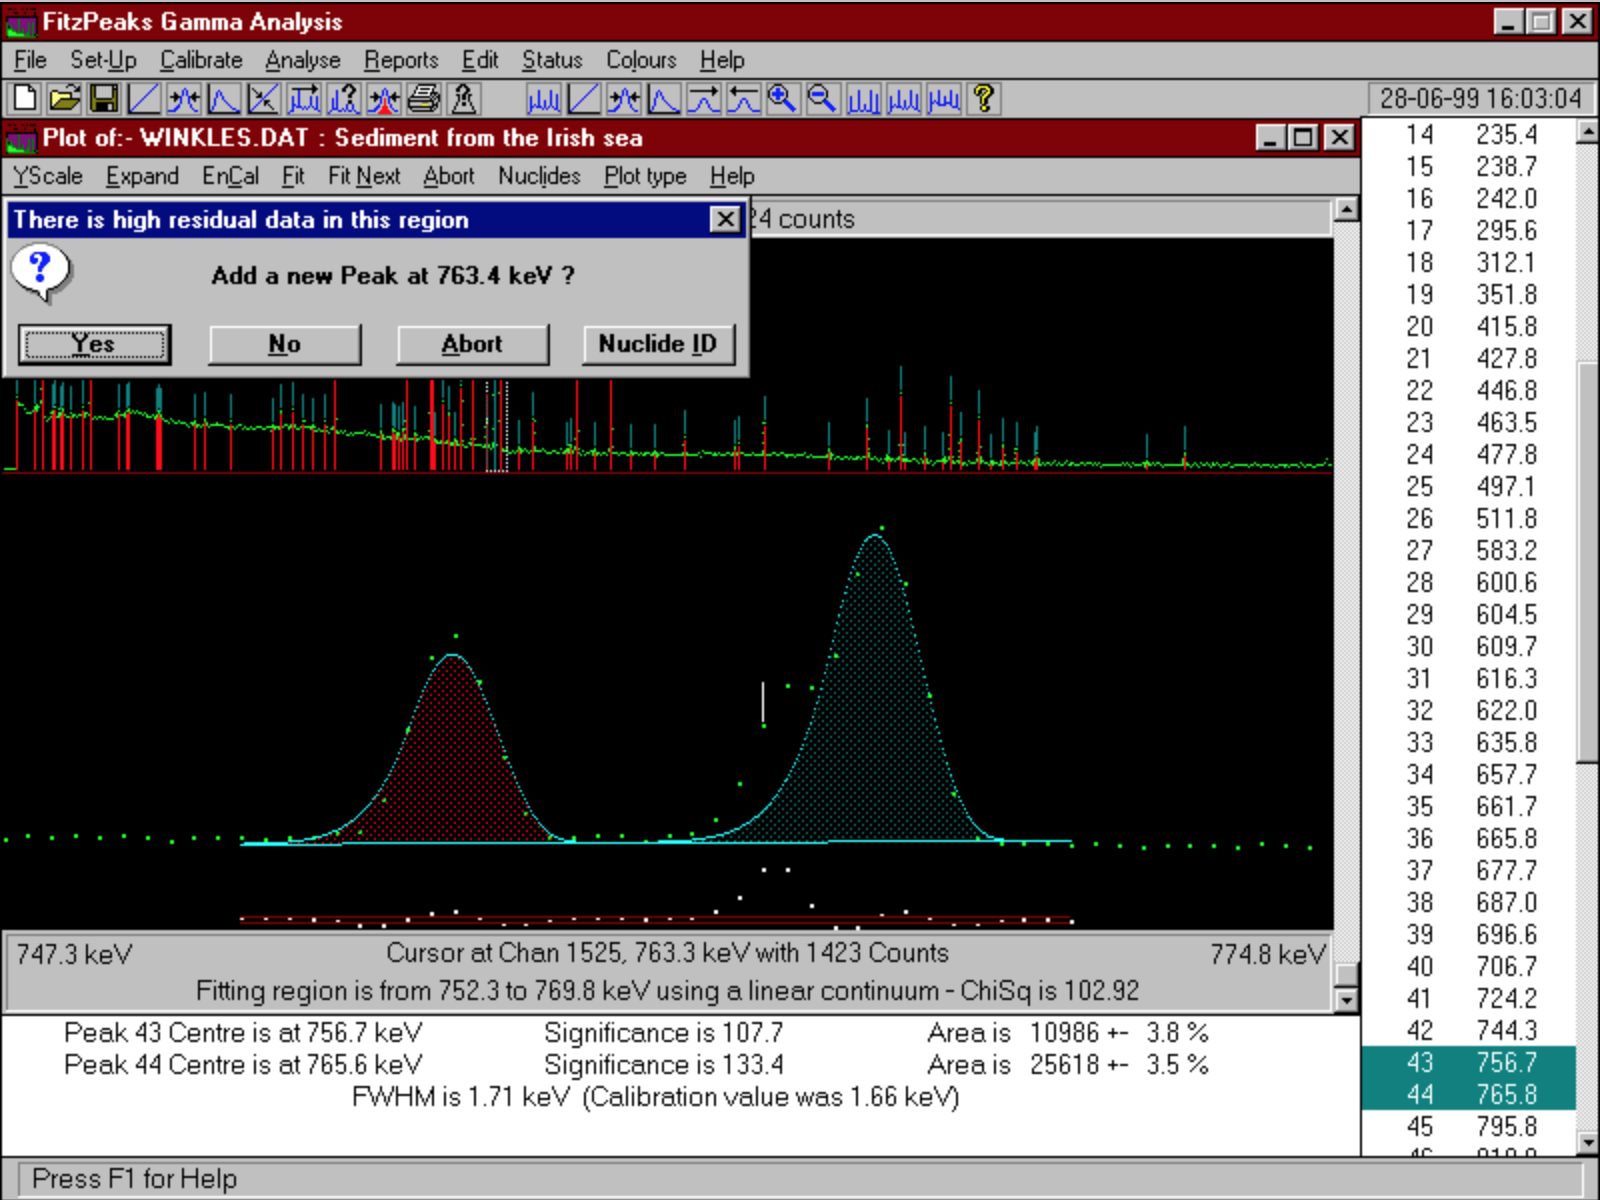
\includegraphics[width=12cm]{Analysis/fitz_example.png}
    \caption{from:http://www.jimfitz.co.uk/pk1_fsz.htm}
    \label{fig:fitz_example}
\end{figure}

\noindent For each spectra, a report file containing peak energy, centre channel, full width half maximum, significance, goodness of fit, peak area and uncertainty in peak area, gammas per second and uncertainty in gammas per second and a background estimation for each peak was provided. The parameters which were used in the analysis was the peak energy for identification, the peak area $N_C$ which was used in the activity equation\ref{eq:Final_Expression_A0} and estimation of efficiency, and uncertainty in peak area. The gammas per second (also referred to as countrate) was used to get an indication of the rate of gammas, which were used as a critical tool to evaluate background contamination in a peak, by comparing to background spectra.  \\ 

\noindent 
Figure \ref{fig:193mPt_spectra} shows the X-ray region (upper) and the gamma-ray region (lower) of $^{193m}$Pt \textcolor{red}{which spectra?} taken approximately .... hours after end of beam. From the lower figure, it is clear that 135.5 keV (0.11 \%) lays on the shoulder of the long-lived $^{192}$Ir ($t_{1/2}$=73.829 d) 136.39 keV (0.199\%) \cite{Baglin2012, ShamsuzzohaBasunia2017a}. 

%The nuclei were identified on behalf of thei're gamma-ray energy. The feeding of multiple nuclei into one gamma-ray peak was avoided by using other gamma-lines. 
\begin{comment}
\begin{figure}
    \centering
    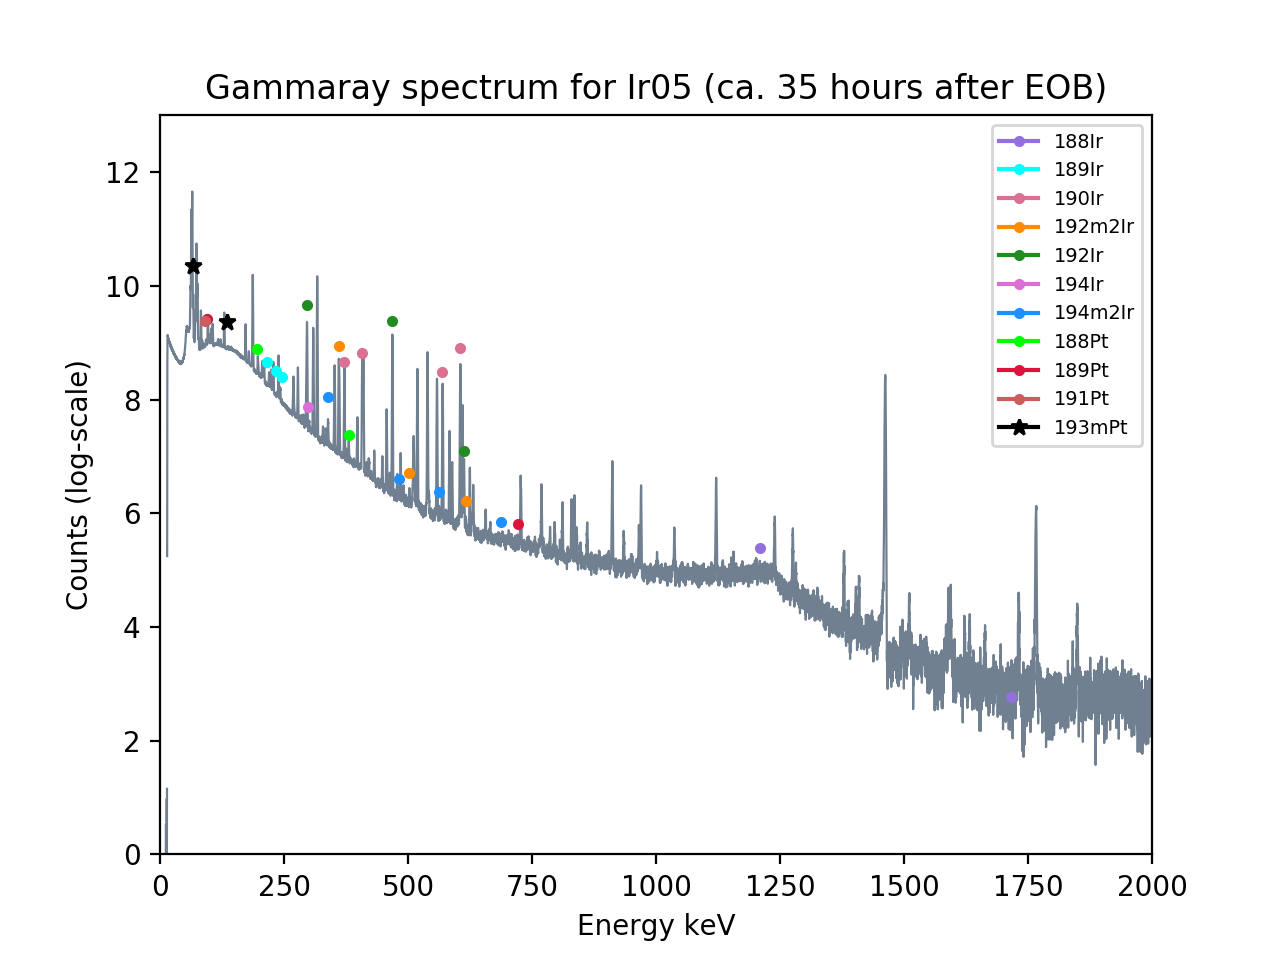
\includegraphics{Analysis/gammaray_spec_Ir05.png}
    \caption{Gammaray spectrum for Ir05 taken approximately 35 hours after end of beam. Nuclei does not necessarily represent what is present in the spectrum, but where the peak would have been. Hard to include all since there are different decay times. \textbf{right:} the total, \textbf{left:}zoomed to show the staircase}
    \label{fig:gammarayspectrum_example}
\end{figure}
\end{comment}


\begin{figure}%
    \centering
    \subfloat[X ray plot of 193mPt. ]{{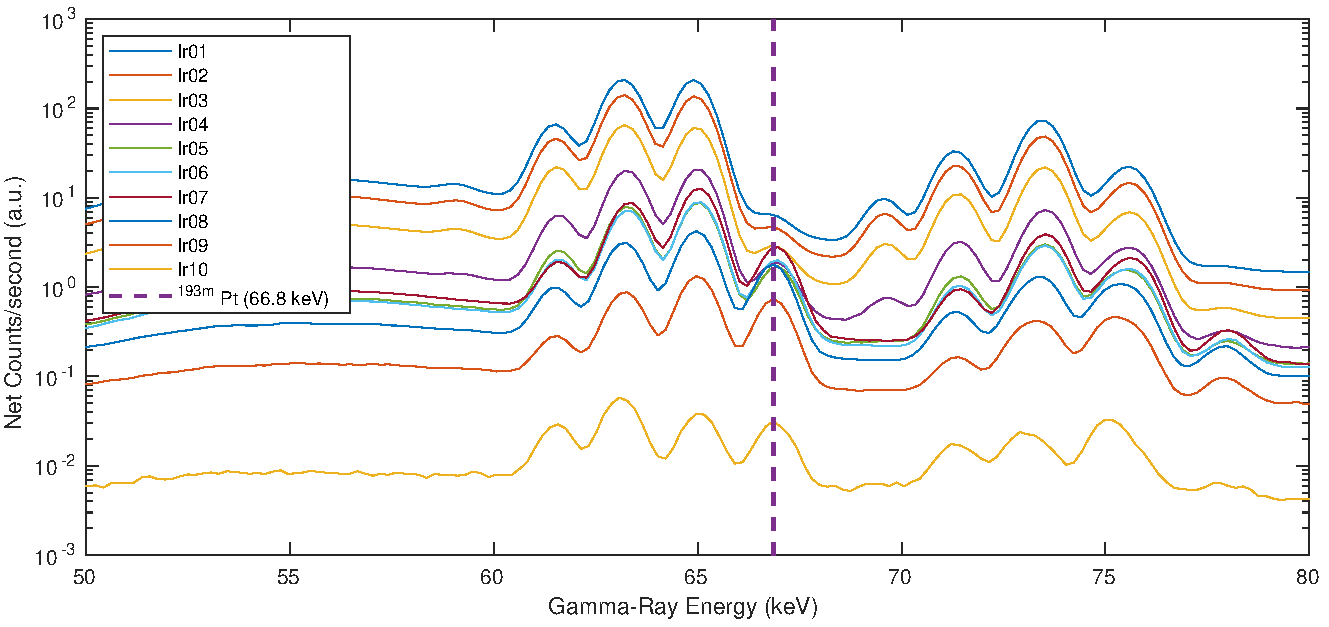
\includegraphics[width=10cm]{Analysis/193mPt_xray_plot.pdf} }}%
    \quad
    \subfloat[Gammaplot of 193mPt]{{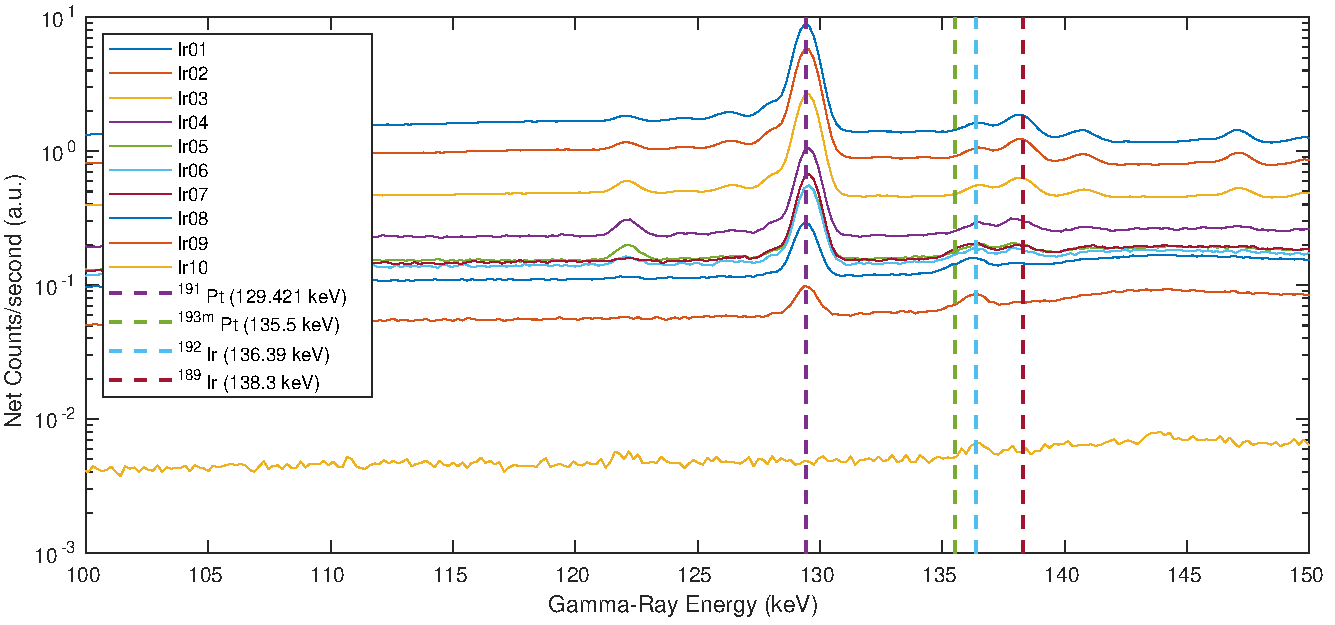
\includegraphics[width=10cm]{Analysis/193mPt_gamma_plot.pdf} }}%
    \caption{\textcolor{red}{Which spectra are these??  }}%
    \label{fig:193mPt_spectra}%
\end{figure}


A matlabscript written by Voyles, A. (2019) was used to loop over all report files for each single spectra in each foil. Gamma-energies with less than \textcolor{red}{0.5 (doublecheck)}  keV in difference were added and averaged, which can be seen on figure \ref{fig:Ir_staircase_gammas} where the channel number is listed on the x-axis and the gamma-ray energy is listed on the y-axis. The result is a staircase where the energies within the tolerance are averaged. This gave a list of gamma-ray energies for each target foil type, one for iridium, one for nickel, one for copper and one for iron. Each of the gamma-lines were identified manually using the nndc-database (Nudat-2.8) \cite{VRAPCENJAKLidijaZERKIN2015}, going through possible reactions based on Q-value, where the Q-value calculator from NNDC was used \cite{PritychenkoB.SonzogniA.NNDC}. If more than one nucleus fed into the same gamma-ray energy within a tolerance of 1 keV, then the peak was not used if there were other possible gamma-ray energies present. If not, the half-lives were compared, and if there was a large difference, only early spectra or very late spectra were used when the activity of the other was not present. In addition, peaks which were contaminated with background radiation was also not used, unless the countrate was very small in comparison to the count-rate of the peak. If it had to be used, the method for background subtraction is described below in subsection \ref{subsec:background_subtraction}. 

For each nucleus identified, the gamma-rays from nndc (listed in tables \ref{tab:Products_Ni}, \ref{tab:Products_Fe}, \ref{tab:Products_Cu} and \ref{tab:Products_Ir} for nickel, iron, copper and iridium respectively) along with half-life, intensity and uncertainty in intensity were gathered. 

\begin{figure}
    \centering
    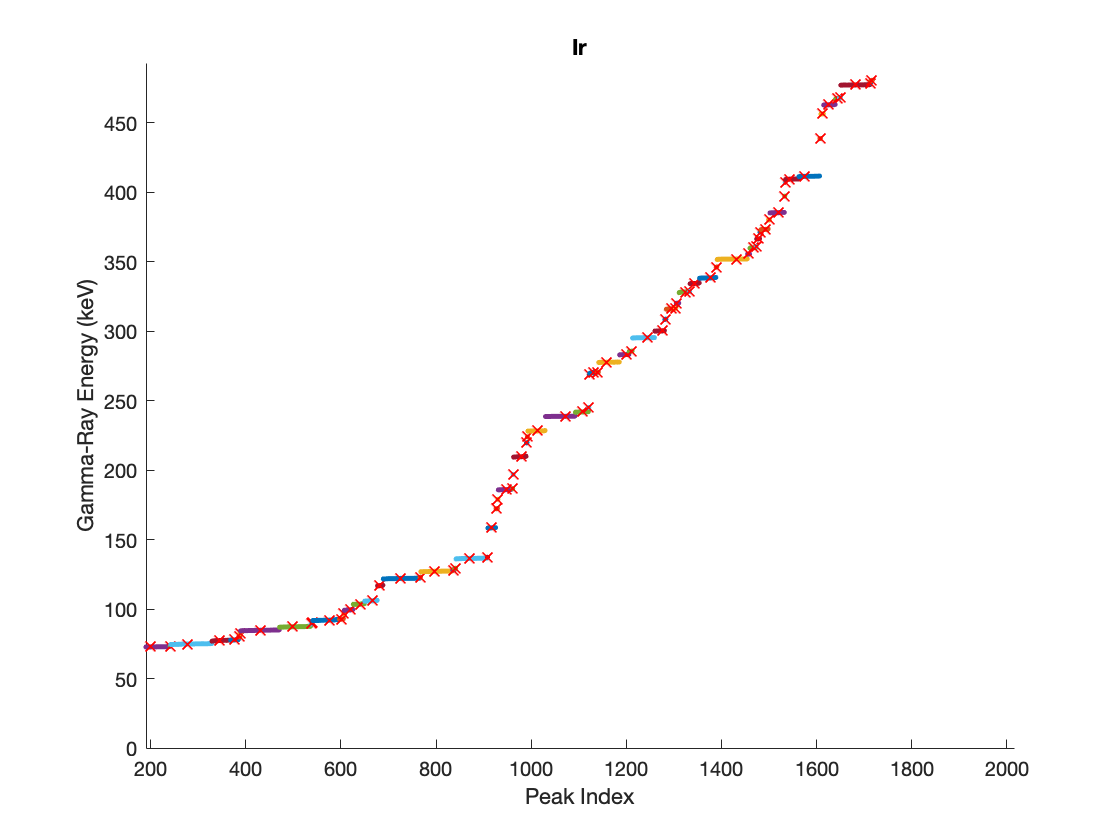
\includegraphics[width=0.8\textwidth]{Analysis/Ir_staircase_zoomed.png}
    \caption{Zoomed staircase for energies between 0 and ca. 500 keV.  Shows how the gamma-rays within  a tolerance of 0.5 keV were averaged. Each "staircase" represents one gamma-ray energy which was used for identification. }
    \label{fig:Ir_staircase_gammas}
\end{figure}

\subsection{Background subtraction} \label{subsec:background_subtraction}
In a few number of cases, background subtraction was necessary due to the presence of some nuclei in the background, which was only problematic for the detectors located in cave 4C. Nuclei of cobalt was in particular present in the background. The general rule of thumb was only to use background subtraction when all gamma-lines of the nucleus was contaminated with a count-rate of the same order, due to the raise in uncertainty. If not, the line was avoided. \\

\noindent 
The count-rate is defined as the number of counts divided by the live time of the spectrum, in units counts/second 

\begin{equation} \label{eq:Countrate}
    C= \frac{N_C}{\Delta t_\text{live}}
\end{equation}

\noindent The number of true counts is the sum of the true gammas and the background 

\begin{equation}
    C_\text{true} = C_\text{obs} - C_{bg}
\end{equation}

\noindent The count-rate in the background spectra are constant, which here is denoted as $C_{bg}$. The observed count-rate is thus the number of true counts divided by the live time of the spectrum and the background count-rate on the detector. From equation \ref{eq:Countrate}, the number of counts are the count-rate multiplied by the live time, which gives

\begin{equation}
    N_\text{true} = N_\text{obs}-(\Delta t_\text{live}C_{bg})
\end{equation}


\begin{comment}
\begin{figure}%
    \centering
    \subfloat{{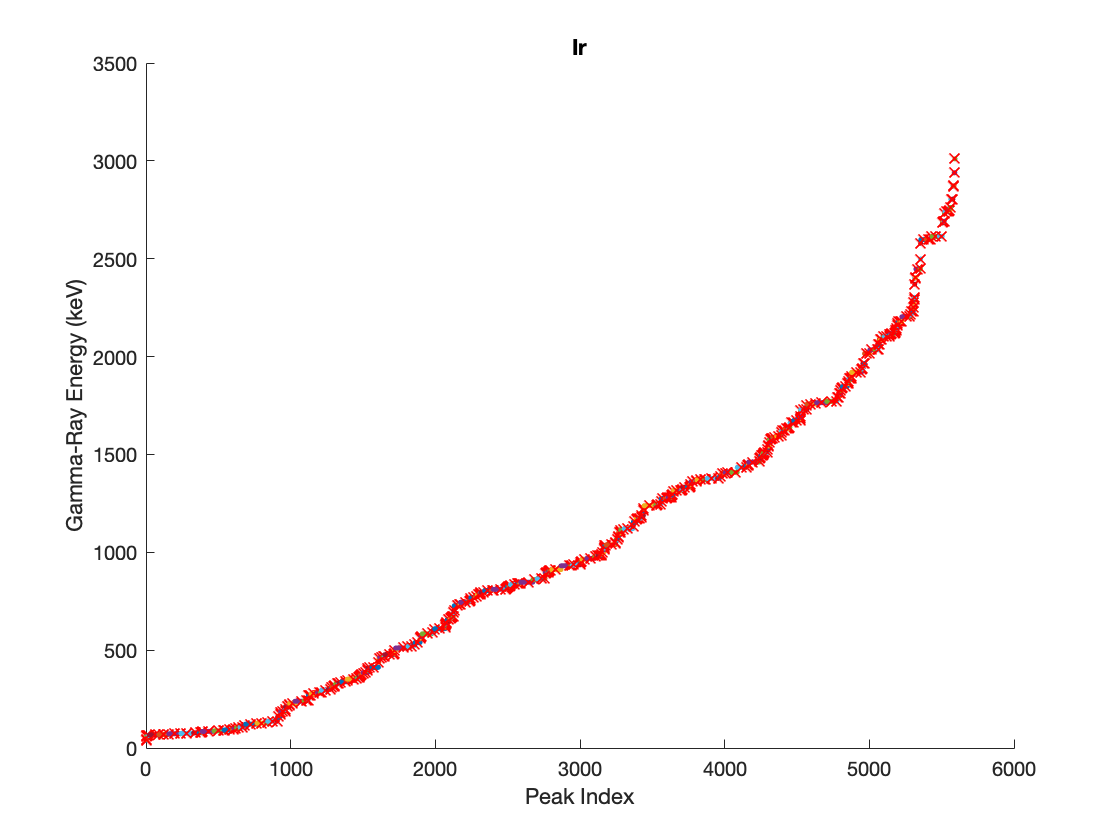
\includegraphics[width=8cm]{Analysis/Ir_staircase.png} }}%
    \quad
    \subfloat{{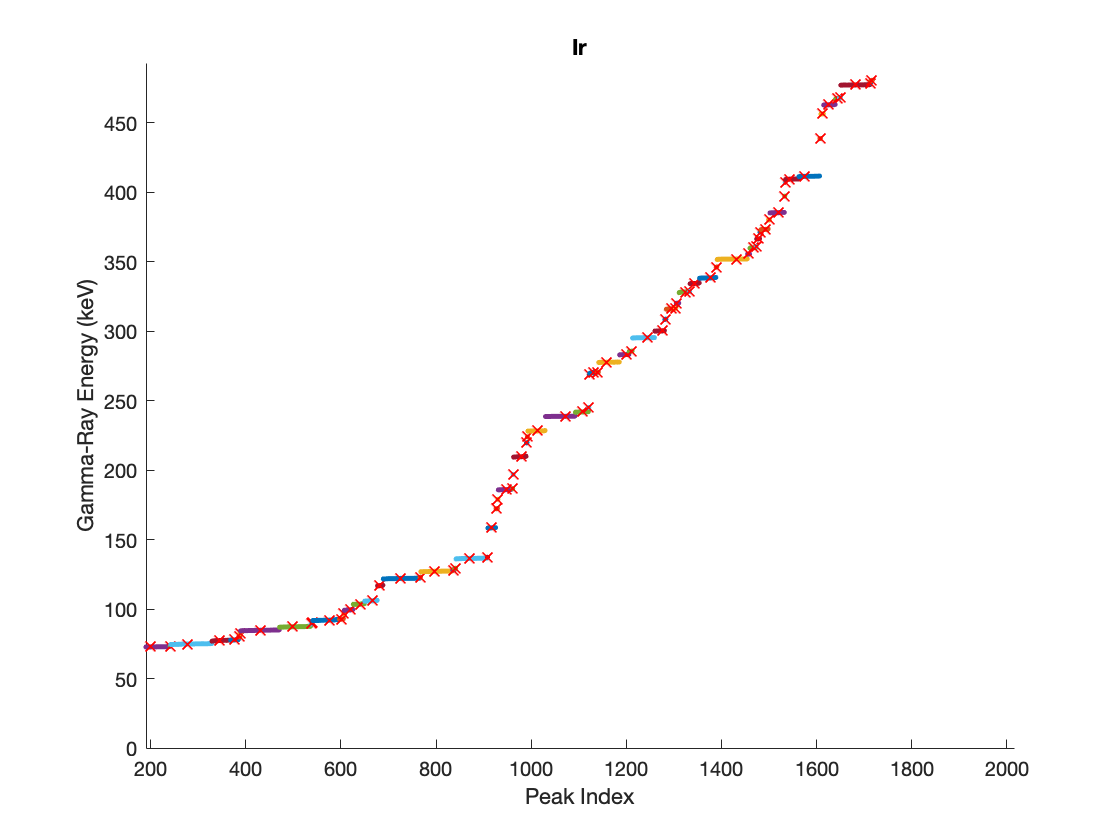
\includegraphics[width=8cm]{Analysis/Ir_staircase_zoomed.png} }}%
    \caption{The figure shows the gamma-lines sorted in a staircase model for iridium.. }%
    \label{fig:Ir_staircase_gammas}%
\end{figure}
\end{comment}





\section{Estimating the end of beam activities}
The end of beam activities were estimated by extrapolating backwards in time with the measured activities at various time points after the end of beam. The activities measured in each spectrum as a function of time since end of beam was calculated using equation \ref{eq:Final_Expression_A} along with a self-attenuation correction:

\begin{equation} \label{eq:activity_eob_matlab}
    A(\Delta t_d) = \frac{N_C\lambda}{\epsilon I_\gamma (1-e^{-\lambda \Delta t_d})e^{-\mu\rho\Delta r/2}}
\end{equation}

where $\mu$ is the photon attenuation coefficients from the XCOM photon cross section database \cite{M.J.BergerJ.H.HubbellS.M.SeltzerJ.ChangJ.S.CourseyR.SukumarD.S.Zucker2010}%\footnote{https://www.nist.gov/pml/xcom-photon-cross-sections-database}
, and $\rho\Delta r$ is the areal density of the foil. The gammas which were used are listed in tables \ref{tab:Products_Fe}, \ref{tab:Products_Ni}, \ref{tab:Products_Cu} and \ref{tab:Products_Ir} for iron, nickel, copper and iridium respectively. The gamma-ray self-attenuation (which is typically less than 0.2 \% \cite{Voyles2019}) correction is based on the assumption that all activity that is made is located midway in the foil thicknesses. In reality however, the activity profile will follow the same shape as the excitation function over the energy range that expands over the foil, \textcolor{red}{if we assume that the stopping power dE/dx=0 which is a good estimation for thin foils less than 100 mg/cm$^2$??} (since activity and cross section are proportional). We do not know the excitation function ahead of time, and the excitation function does not change much either, since the foil thicknesses are so thin. So instead, this simplification is done, assuming that the average attenuation is through half of the foil thickness. \\ 

In a matlabscipt written by Voyles, A. S (2020), the gamma-ray energies used, and intensity, uncertainty in intensity and half-life were assigned to each nucleus. Each foil type and foil number was looped over to see if the observed gamma-ray within a tolerance of 0.5 keV was registered, and with the number of counts, uncertainty in number of counts, the time since end of beam, the areal density and mass attenuation correction, and the efficiency which was dependent on which detector, the activity at each observed time point since end of beam was calculated according to equation \ref{eq:activity_eob_matlab}. The result was an output file for each foil with the calculated activity according to equation \ref{eq:activity_eob_matlab} with hours since end of beam. The output files were read into a separate program for calculation of the end of beam activities. The uncertainty in each measured activity was the quadruple sum (calculated according to equation \ref{eq:uncertainty_simplification}) for the number of counts, the efficiency, the intensity and half-life (provided by the IAEA database \cite{VRAPCENJAKLidijaZERKIN2015}) and the uncertainty in the areal density for each foil. The main contributing factors of the uncertainty was the number of counts in the peak and the uncertainty in efficiency calibration which varied as a function of energy (figure \ref{fig:rel_uncertainty_efficiency}). Some of the measured activities were nonphysically large, and error searches to find the source of high activity was done for each product nucleus. \textcolor{red}{It appeared that the efficiency for detector 2 at 30 cm had an efficiency which can be too high that contributes to those values}. If the values were larger with several orders of magnitude, than the rest of the calculated activities, and the error-search dit not give any clarity of what was causing the high activities, the points were not used in the analysis. \\ %, dependent on the feeding or ..., the activities at the various timepoints were used to extrapolate backwards in time to estimate the end of beam activity at time =0. The more datapoints, the more sure we could be that the data was good. \\ 


The activity curves are based on Bateman equations \cite{PopO.M.SimulikV.M.2016}. The decay curve of single a radioactive nucleus takes an exponential form

\begin{equation} \label{eq:singledecay}
    A(t_d)=A_0 e^{-\lambda t_d}
\end{equation} 
where $t_d$ is the delay time (here since end of beam), $A_0$ is the activity right after end of beam. For multiple decay, Bateman equation is used describing the activity in nucleus n of the decay chain

\begin{equation} \label{eq:ndecay_chains}
    A_n = \lambda_n \sum_{i=1}^n \Big[ \Big( A_{i,0}\prod^{n-1}_{j=i}\lambda_j \Big)\cdot \Big( \sum_{j=i}^n \frac{e^{-\lambda_j t}}{\prod_{i\neq j}^n (\lambda_i - \lambda_j)} \Big) \Big]
\end{equation}

where $A_n$ is the activity of nuclei n in the decay chain, with the corresponding decay constant $\lambda_n$. The equation sums over all nuclei in the decay chain. $A_{i,0}$ is the initial activity of nucleus i, and j is the nucleus which is feeding into nucleus i. In this work, decay chains of single and two-step (n=1,2) were sufficient. For two-step decay, equation \ref{eq:ndecay_chains} takes the form

\begin{equation} \label{eq:twostep_activity}
    A_d(t) = \lambda_n \Big[ A_{p,0}\lambda_1 \frac{(e^{-\lambda_1 } + e^{-\lambda_d})}{\lambda_p - \lambda _d} + A_{d,0}e^{-\lambda_d t} \Big],\quad \text{two step decay}
\end{equation}

where subletter p is shortened for parent is the parent nucleus, and subletter d is shortened for daughter. The parent activity is calculated from single step decay. \\

%The equation describing the shape of the decay curve is given in equation \ref{eq:activity_decaylaw} for single decay or \ref{eq:ndecay_chains} for multiple decay. Decay chains of single and two-step decay (n=1,2) was sufficient in this analysis; 
%\begin{equation} \label{eq:onestep_activity}
 %   A = A_0 e^{-\lambda \Delta t_d},\quad \text{ single step decay}
%\end{equation}

%and

%\begin{equation} \label{eq:twostep_activity}
%    A_2(t) = \lambda_n \Big[ A_{1,0}\lambda_1 \frac{(e^{-\lambda_1 } + e^{-\lambda_2})}{\lambda_1 - \lambda _2} + A_{2,0}e^{-\lambda_2 t} \Big],\quad \text{two step decay}
%\end{equation}



\noindent The extrapolation was done using the scipy optimize curvefit function \cite{Virtanen2020}, where the activities and the uncertainties in activities calculated from equation \ref{eq:activity_eob_matlab} were fitted to the decaycurve, minimizing the $\chi^2$, with the end of beam activity serving as optimizing parameter. The function returns the optimal parameters along with the estimated covariance matrix of the optimal parameters. For the cases where there was twostep feeding, but the parent nucleus did not emit observable gamma-rays, twostep decay with both the end of beam activities of the daughter and the parent served as optmizing parameters was used. For the two former cases, there was only one optimizing parameter, and the uncertainty was estimated using the squareroot of the covariance matrix (V). 
\begin{equation}
    \delta_{A_0}=\sqrt{{V}}
\end{equation}

For the latter, the two optimizing parameters are correlated, and equation \ref{eq:variance_full} had to be used to estimate the uncertainty. 


%The extrapolation was done using the scipy optimize curvefit function , where the $A_0$ of the daughter was the optimizing parameter. Since there is only one optimized parameter, there was no covariance and the uncertainty was calculated using equation \ref{eq:uncertainty_simplification}. In the cases where neither parent or daughter activity were known, which were the single case for the monitor reaction $^{58}Co$ with $^{58m}$Co decaying into the ground state by internal conversion, both parent and daughter activity were optimizing parameters which are very correlated and thus the uncertainty in end of beam activity was calculated \ref{eq:variance_full}. \\

\noindent 
Figure \ref{fig:activity_curves} shows three examples of three different activity curves; one step decay for $^{193m}$Pt ($t_{1/2}$=4.33 days), two step decay decay for $^{58}$Co ($t_{1/2}$=70.86 days) with feeding from the isomer $^{58m}$Co ($t_{1/2}$=9.10 hours), which had to be fitted using two optimizing parameters, and twostep decay of $^{56}$Co ($t_{1/2}$=77.236 d) with feeding from $^{56}$Ni ($t_{1/2}$=6.075 d) using the activity of $^{56}$Ni and the optimized parameter of $^{56}$Co. The uncertainty bands are large for $^{58}$Co, as the twostep decay with no observed parent contributes to a higher uncertainty.


\begin{figure}%
    \centering
    \subfloat{{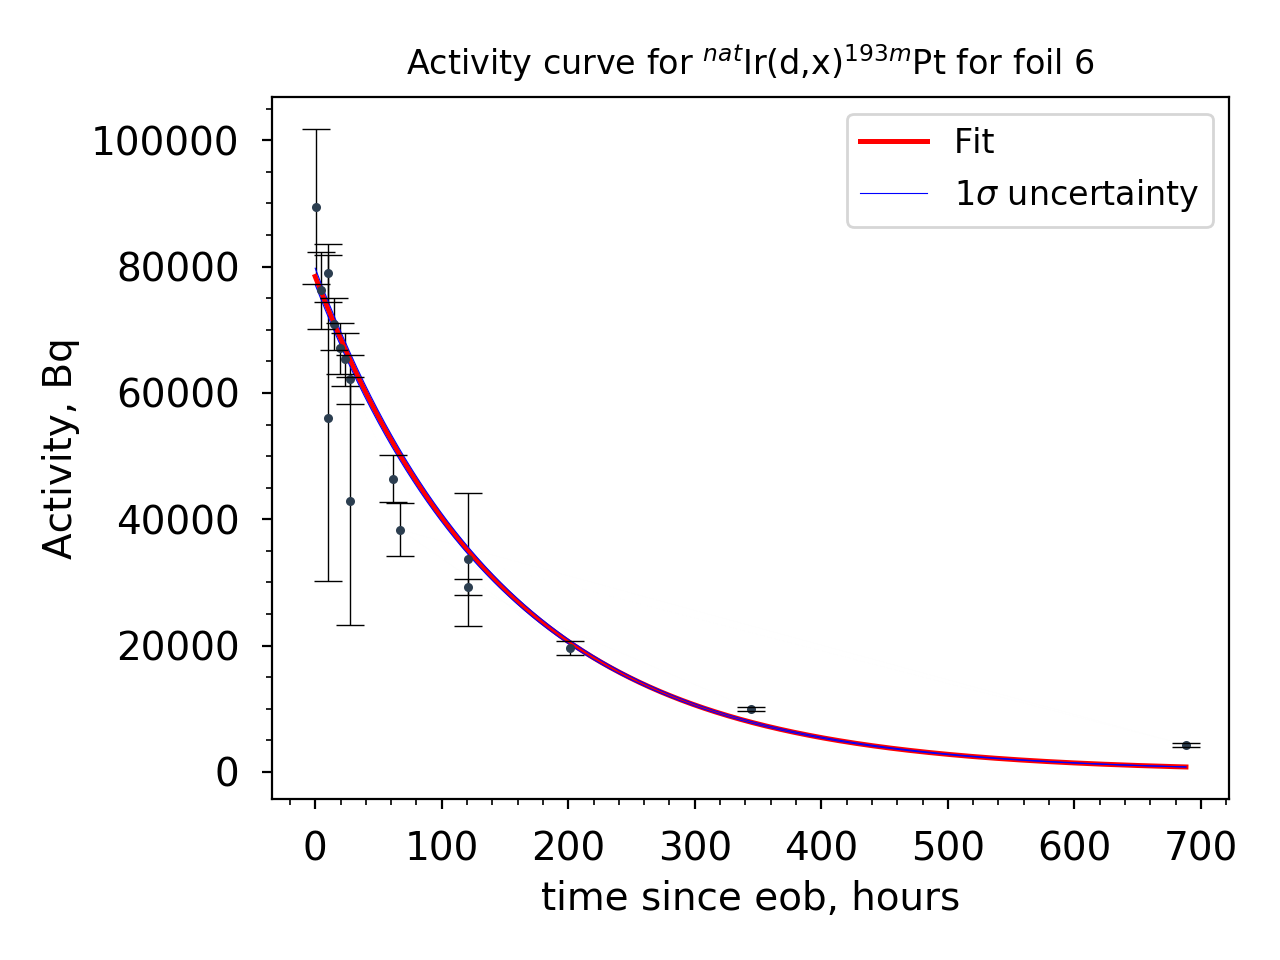
\includegraphics[width=11cm]{Analysis/activity_Ir_193mPt_f6.png} }}\hfill
    \subfloat{{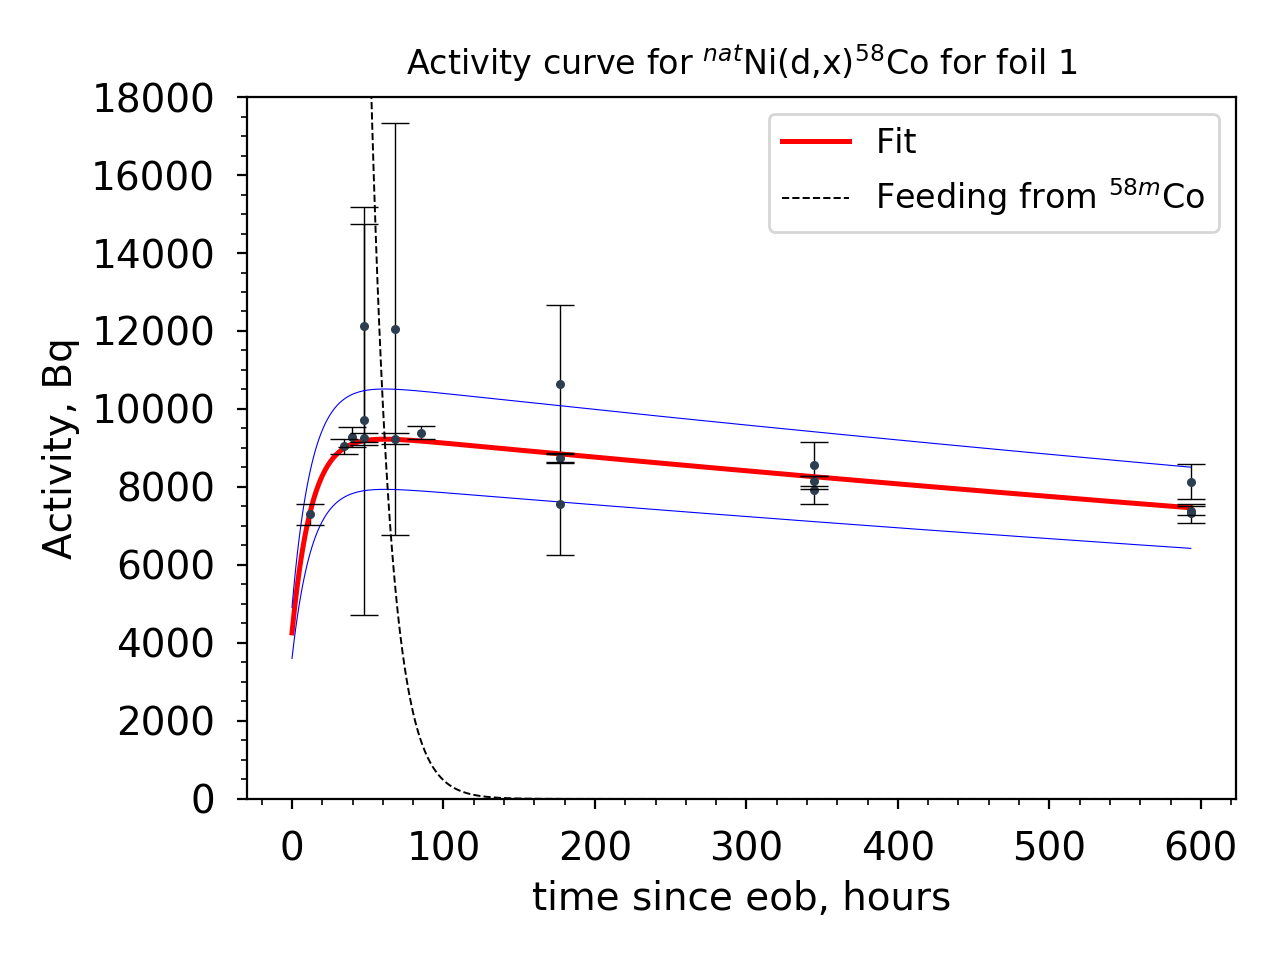
\includegraphics[width=7cm]{Analysis/activity_58Co.png} }}%
    \subfloat{{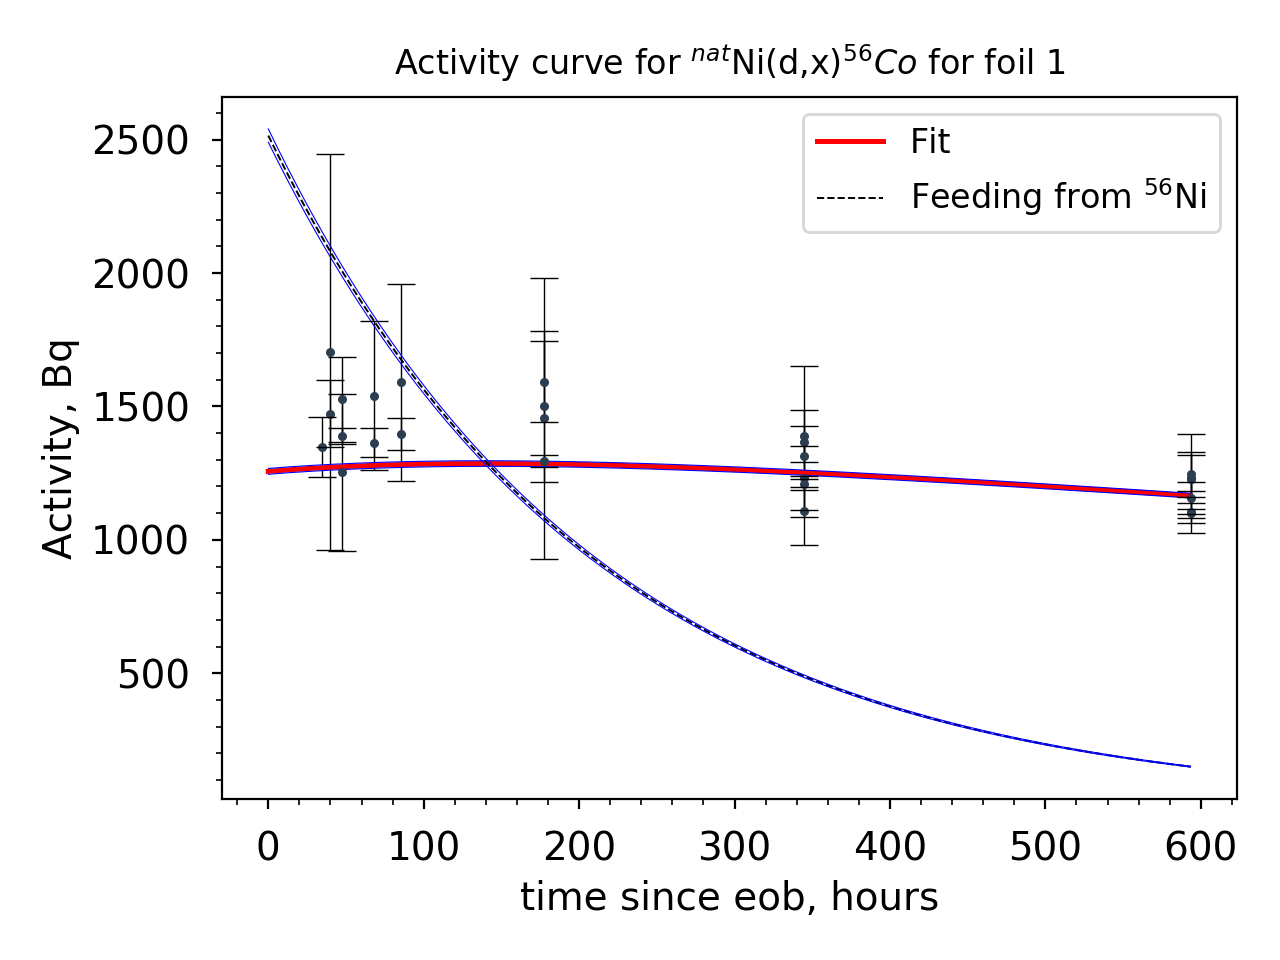
\includegraphics[width=7cm]{Analysis/activity_56Co.png} }}%
    \caption{Examples of three activity curves. \textbf{Top:} Onestep decay for $^{193m}$Pt ($t_{1/2}$=4.33 days), extrapolated with equation \ref{eq:onestep_activity}. \textbf{Bottom left:} Twostep decay for $^{58}$Co ($t_{1/2}$=70.86 d) with feeding from the isomer ($t_{1/2=9.10}$ h, IT:100\%). The curve was extrapolated using twostep decay (equation \ref{eq:twostep_activity}) with both daughter and parent as optimizing parameters. \textbf{Bottom right:} Twostep decay for $^{56}$Co ($t_{1/2}$=77.236 d) with feeding from $^{56}$Ni ($t_{1/2}$=6.075 d, $\epsilon$:100\%).     }%
    \label{fig:activity_curves}%
    
\end{figure}
%\subsection{Activities of the monitor foils}
%The activities of the monitor foils were important 
%\subsection{$^{193m}$Pt}

\section{Monitor reactions}
The requirement of monitor reaction-data used to estimate beam current or flux for beam-monitor reactions is well-characterized cross sections, provided by the IAEA Coordinated research Project on "Nuclear Data for Charged-particle Monitor Reactions and Medical Isotope Production" where an international team between 2012-2017 worked to evaluate a limited number of cross section data which was in well-agreement \cite{Hermanne2018a} for recommended cross sections used to estimate monitor beam current. The recommended curves are interpolations over the recommended data, fit to an analytical approximation based on the ratio of two polynomials, with uncertainties obtained using the co-variance matrix, where the "full diagonal form represents a dataset in which each point possesses independent uncertainty"\cite{Hermanne2018a}, p. 344. In addition, a systematic uncertainty of 4\% was added. In addition to yielding precise cross section measurement as a function of beam energy, it was important that the neutron originating from deuteron break-up did not cause the induced activity for monitor reactions to increase, giving a higher beam energy than the true one (along with break-up protons but because of the positive charge, it is stopped quickly). For the reactions, the only possible neutron induced reactions are from $^{56,58}$Co, but analyzing the Ni-monitor foil in the back of the stack, there was no evidence of these two reactions, so that impact was not ......  \\ 

The activity for each monitor-reaction was obtained by using the gamma-lines listed in table \ref{tab:monitor_reactions}. More gamma-lines were included than the recommended listed \cite{Hermanne2018a}. In the back-propagation fit of activities, more data gives a better statistical precision. However, some of the activities at time points after end of beam got calculated specific gamma-lines had nonphysically high activity in comparison to the other measured. These were not used and excluded from the back-propagation fit. \\

%\centering    
\newpage
    \begin{longtable}{|c|c|c|c|c|}
    \caption{The table shows an overview of the gamma-lines used to estimate the activation in each foil at the end of beam. Nuclear data from: \cite{Junde2011, Nesaraja2010a, Zuber2015, Nichols2012, ERJUN2001, Browne2010a}.}\\
    \hline
    \makecell{Monitor reaction} & \makecell{Half-life} & \makecell{Gamma-lines (keV)} & \makecell{Intensity (\%)} & \makecell{Useful beam-energies(MeV)  \cite{Hermanne2018a}}  \\
    \hline
    \makecell{$^\text{nat}$Fe(d,x)$^{56}Co$} & \makecell{77.236 d} & \makecell[t]{263.434 \\ 486.55 \\ 733.514 \\ 787.743 \\ 846.770 \\ 852.732 \\ 896.510 \\ 977.372 \\ 996.948 \\ 1037.843 \\ 1140.368 \\ 1159.944 \\ 1175.101 \\ 1198.888 \\ 1238.288 \\ 1335.40 \\ 1360.212 \\ 1771.357 \\ 1963.741 \\ 2015.215 \\ 2034.791 \\ 2212.944 \\ 2276.131 \\ 2598.500} & \makecell[t]{0.0220 \\ 0.0540 \\ 0.191 \\ 0.311 \\ 99.9399 \\ 0.049 \\ 0.073 \\ 1.421 \\ 0.111 \\ 14.05 \\ 0.132 \\ 0.094 \\2.252 \\ 0.049 \\ 66.46 \\ 0.1224 \\ 4.283 \\ 15.41 \\ 0.707 \\ 3.016\\ 7.77 \\ 0.388 \\ 0.118 \\ 16.97 }  & \makecell{10-50}\\ 
    \hline
    \makecell{$^\text{nat}$Ni(d,x)$^{56}$Co (cum)} & \makecell{77.236 d}  & \makecell[t]{787.743 \\846.770\\ 977.372 \\ 1175.101 \\ 1963.741 \\ 2015.215 \\ 2034.791} & \makecell[t]{0.3111 \\ 99.9399 \\ 1.421 \\ 2.252 \\ 0.707 \\ 3.016 \\ 7.77} & \makecell{5-50} \\
    \hline
    \makecell{$^\text{nat}$Ni(d,x)$^{58}$Co (cum)} & \makecell{70.86 d} & \makecell[t]{-1823.8 \\ 6084.9 \\-1735.3 \\-12331.0\\ -28826.2}   & \makecell[t]{810.7593\\ 863.951 \\1674.725 } & \makecell{5-50}  \\
    \hline
    \makecell{$^\text{nat}$Ni(d,x)$^{61}$Cu} & \makecell{3.339 h} & \makecell[t]{282.956 \\ 373.050 \\ 529.169\\ 588.605 \\ 625.605 \\ 656.008 \\ 816.692 \\ 841.211 \\ 902.294 \\ 1032.162 \\ 1073.465 \\ 1132.351 \\ 1185.234 \\ 1446.492} & \makecell[t]{12.2 \\ 2.1 \\ 0.38 \\ 1.17 \\ 0.040 \\ 10.8 \\ 0.31 \\ 0.21 \\ 0.083 \\ 0.043 \\ 0.033 \\ 0.090 \\ 3.7 \\ 0.045} & \makecell{3-50}  \\
    \hline
    \makecell{$^\text{nat}$Cu(d,x)$^{62}$Zn)} & \makecell{9.193 h} & \makecell[t]{40.85 \\ 243.36 \\ 246.95 \\ 260.43 \\ 304.88 \\ 394.03 \\ 548.35 \\ 596.56 \\ 637.41} &  \makecell[t]{25.5 \\ 2.52 \\ 1.90 \\ 1.35 \\ 0.29 \\ 2.24 \\ 15.3 \\ 26.0 \\ 0.25} & \makecell{15-50}  \\
    \hline
    \makecell{$^\text{nat}$Cu(d,x)$^{63}$Zn} & \makecell{38.47 m} & \makecell[t]{449.93 \\ 669.62 \\ 962.06} & \makecell[t]{0.236 \\ 8.2 \\6.5 } & \makecell{8-50}  \\
    \hline
    \makecell{$^\text{nat}$Cu(d,x)$^{65}$Zn} & \makecell{243.93 d} &\makecell[t]{1115.539} & \makecell[t]{50.04} & \makecell{5-50} 
    \hline
    \label{tab:monitor_reactions}
    \end{longtable}{|c|c|c|c|c|}


\section{Deuteron beam current and energy assignment} \label{sec:beamcurrent}
The beamintegrator measured a current of 128.5 nA in front of the beam stack. However in order to have precise cross section measurements, the nominal beam current in each foil was calculated. \textcolor{red}{As the beam loses energy throughout the stack via collisions, the deuteron beam will have a certain broadening due to the small angle deflections}. The IAEA recommended monitor reactions $^\text{nat}$Ni(d,x)$^{61}$Cu,$56,58$Co, $^\text{nat}$Cu(d,x)$^{62,63,65}$Zn and $^\text{nat}$Fe(d,x)$^{56}$Co \cite{Hermanne2018a} were used to obtain a weighted average beam current in each foil solving equation \ref{eq:Final_Expression_A0} for beam current $\Phi$:

\begin{equation} \label{eq:BC_simple}
    \Phi(E_d) = \frac{A_0}{N_T \sigma(E_d)_\text{mon}(1-e^{-\lambda \Delta t_\text{irr}})}
\end{equation}
\noindent 
where the units are deuterons per second, $E_d$ is the deuteron energy (MeV), $A_0$ is the end of beam activity (Bq) estimated from the spectra for each monitor reaction, $N_T$ was calculated from the mass densities, and $\sigma(E)$ is the monitor data from the IAEA database. In the assumption that the deuteron beam current should not be degraded within the same compartment, it is possible to use multiple monitor reactions to determine the average beam current in each compartment, which gives a higher probability that the true beam current is found. This is provided that the simulated energy distributions are accurate \cite{Graves2016}. As stated by Graves et. al. (2016), this method of using multiple monitor reactions has the potential of reducing the uncertainties in the deuteron energy towards the end of the stack. \\

Equation \ref{eq:BC_simple} builds upon the thin target assumption, which implies that the energy degradation in the foil is zero. However, we know that there is an energy distribution, which was estimated using NPAT's (Nuclear Physics Analysis Tool) Ziegler simulation \cite{MorellJ.}. The Ziegler code simulates the deuteron transport in a Monte-Carlo based simulation, based upon the Anderson \& Ziegler stoppingpower mode\cite{Ziegler1999}. The code was ran with $1\cdot 10^6$ particles with a maximal number of steps being 100. The built in uncertainty in the deuteron energy was set to 0.5 MeV. Anderson \& Ziegler is an empirical stopping power model, and takes the nuclear stopping-power (inelastic and elastic collisions), the electronic stoppingpower and the effective charge of the ions into account (\cite{Backlin1986}, p. 96). Bethe-Block which is known as the stopping-power equation for heavy charged particles {equation \ref{eq:betheblock}} only takes the electronic stopping power into account. % \textcolor{blue}{The elastic interaction between the ion and target is described by means of scattering cross sections in transport and Monte Carlo simulations. The elastic collisions cause both angular deflections and stopping of the ions. The inelastic interactions are conventiently collected into mean values such as the electronic stooping cross section and electronic energy loss straggling because of the alarge variety of possible discrete collisions between the ion and the target electrons. Ions slowing down is included this way, but ion scattering is neglected because of the electron mass. 
Since both elastic and inelastic collisions are statistical events, the range is represented as a distribution (\cite{Backlin1986}, p. 126-126). % Even neglecting the angular deflections the elastic collisions alone would result in a range distribution because there is a spectrum of elastic energy losses. (\cite{Backlin1986}, p. 126-126) %does not have any physics derivation behind it, and is a tuned model which reproduces experimental data. Bethe-Block is derived from basic E\&M with no tuned parameters. Bethe-Block also gives the purely electronic stopping power, the stopping power from an ion's interaction with the electronic cloud of an atom in the stopping medium. However the total stopping power is the sum of electronic, nuclear (elastic and inelastic scattering) and radiative stopping power, which is what we actually want from the experimental standpoint. Bethe-Block ignores nuclear and radiative.  
The code provides the full deuteron energy and flux spectra \textcolor{red}{distribution?} in each foil, $d\phi/dE$, which can be visualized for the iridium foils in figure \ref{fig:ir_energyflux}. From the figure, it can be seen that as the deuteron energy is degraded through the stack, the mean value is shifted towards the low energy side of the peak along with an increasing energy-flux profile width. Because the stopping power is inversely proportional to the charged particle energy (From Bethe-Block, $-\frac{dE}{dx}\propto \frac{1}{\beta^2}$), and the increasing degree of scattering towards the back of the stack, the low energy side of the flux is more degraded than the high energy side, creating a low energy tail, and a shift of the mean value (centroid) to lower energies. The shift causes a higher uncertainty in the energy for the lower energies. The (normalized) flux-weighted average energy for each foil was calculated, which takes the slowing down of deuterons and gives the effective energy centroid in each foil \cite{Voyles2019}, using the energy distributions $d\phi/dE$ provided by the Ziegler code:

\begin{equation} \label{eq:flux_weighted_average_energy}
    \langle E \rangle = \frac{\int E \frac{d\phi}{dE}dE}{\int \frac{d\phi}{dE}dE}
\end{equation}



%the deuteron energy is degraded, the mean value is shifted towards the low energy side, and the the peak width increases. As stoppingpower is inversely proportional to the charge particle energy ($-\frac{dE}{dx}\propto \frac{1}{\beta^2}$), and along with scattering taking place towards the end of stack, the low energy tail is more degraded, and we see a skew towards the low energy, creating a broader energy-flux profile and a shift of the mean value (centroid). This shift leads to an increasing uncertainty in energy. The (normalized) flux-weighted average energy for each foil was calculated, \textcolor{blue}{ironpaper: which takes into account the slowing down of of deuterons, and reports effective energy centroid of each foil}, using the energy distributions $d\phi/dE$ provided by the Ziegler code:

%\begin{equation} \label{eq:flux_weighted_average_energy}
%    \langle E \rangle = \frac{\int E \frac{d\phi}{dE}dE}{\int \frac{d\phi}{dE}dE}
%\end{equation}

\noindent 
The uncertainty in beam energy is divided into low energy and high energy tale, with the FWHM split by the centroid (figure \ref{fig:ir_energyflux}). \\ 

\noindent 
Likewise, the energy-dependent monitor IAEA cross-sections need to be flux-weighted over each foil. This was done using the Scipy interpolation (splrep and splev) function with the smoothing condition set to zero, and the order of derivative set to zero \cite{Virtanen2020}. The energy array over each foil provided by the Ziegler simulation was spline interpolated with the IAEA recommended cross section data. Thus, the monitor cross section term in equation \ref{eq:BC_simple} is modified to 


\begin{equation}
    \sigma (\langle E\rangle) = \frac{\int \sigma_\text{mon} \frac{d\phi}{dE}dE}{\int \frac{d\phi}{dE}dE}
\end{equation}


\begin{figure}
    \centering
    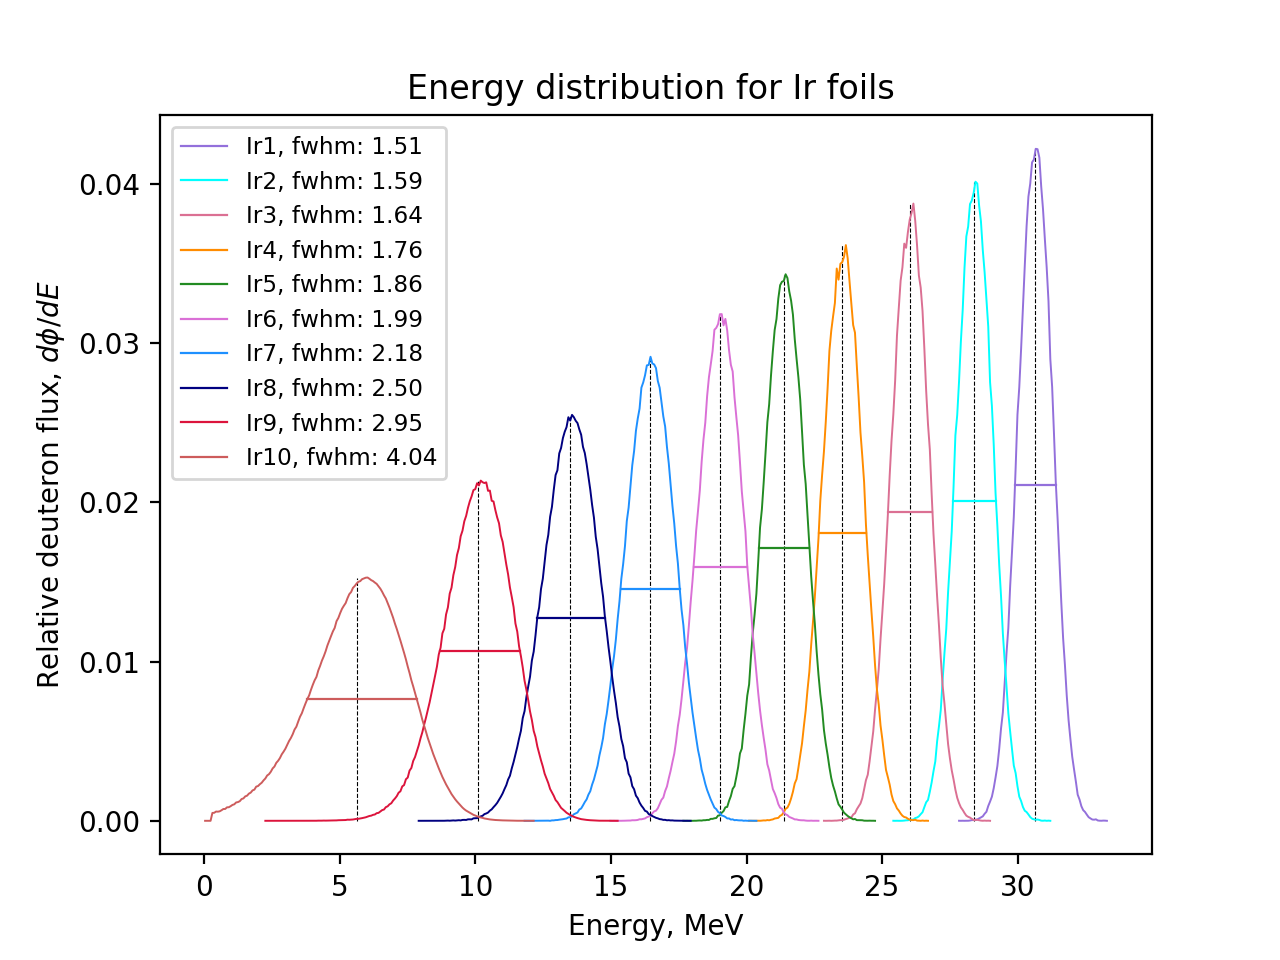
\includegraphics{Analysis/Ir_flux_distribution_B_+2_D_+4,25.png}
    \caption{Iridium energy flux distribution over the 10 foils. As the energy degrades, skewed and larger full width half max. The vertical line in each peak is the mean value. This indicates that at lower energies, the right uncertainty is greater than the left uncertainty in the peak.}
    \label{fig:ir_energyflux}
\end{figure}

The estimated beam-current for each monitor reaction in each foil was calculated using equation \ref{eq:BC_simple} with the modified terms for cross section and beam energy. The uncertainty for the beam-current in each reaction was calculated as the quadruple sum of each term (equation \ref{eq:uncertainty_simplification}). The weighted averaged beam current was estimated \textcolor{red}{Andrew: I dont understand how you did the weighted average in your python script. You did not use the numpy function...}, and the uncertainty in in each parameter was calculated according to equation \ref{eq:variance_full}, since each measured beam-current was co-varianced. Figure \ref{fig:varmin_beamcurrent} (upper) shows the estimated beam current for each reaction in each foil with the measured areal densities and the 33 MeV deuteron beam. However, as we can see in the figure, the spread of the predicted beam current is quite large. The measured values of the beam current, especially in the back of the stack can be due to energy bins being assigned wrongly in the energy distribution simulation done in Ziegler-code or a systematic errors in the areal density which increases further back in the stack \cite{Voyles2018c}. A way to work around this was to perform a variance minimization to find the correct energybins matching to the IAEA monitor cross sections, described in the next section.  

\begin{comment}
With the end of beam activities for the monitor reactions, number of target nuclei and the flux- weighted IAEA cross sections, the beam current as a function of the flux-weighted average beam energy was estimated for each reaction in each foil. 
\begin{equation}
    -\frac{dE}{dx}=2\pi N_a r_e^2 m_e c^2\rho \frac{Z}{A}\frac{z^2}{\beta^2}\Big[\ln \Big( \frac{2m_e \gamma^2 v^2 Q_\text{max}}{I^2} \Big)-2\beta^2 -\delta - 2 \frac{C}{Z}\Big]
\end{equation}
where $r_e$ is electron radius, $m_e$ electron mass, $N_a$ avogadro, I mean excitation potential, Z \& A atomic number and mass numer of absorbing material, $\rho$ density of absorbing material, z charge of incident particle, $\beta=v/c$, $\gamma=1/\sqrt{1-\beta^2}= 1/\sqrt{1-v^2/c^2}$, $\delta$ density correction, C shell correction, $W_\text{max}$ is max energy transfer per collision. In general, $$\frac{dE}{dx}\propto \rho,\frac{z^2}{\beta^2},\frac{Z}{A}$$ and logarithmic stuff which i dont know... so alpha particles are stopped quicker than protons if they have the same energy (Techniques for Nuclear and Particle physics experiments, p. 24). 
Particles interact differently in a given medium. 
\end{comment}

\subsection{Variance minimization for the deuteron energy assignments}
In theory, the estimated beam current of a charge particle beam should be constant, until completely stopped, since the majority of the incident particles does not interact in nuclear reactions, but only lose energy via elastic and inelastic scattering. This method has the potential to reduce the deuteron uncertainty in the foils in the back of the stack, where the effects of energy straggling ..... ??? Graves et. al. Variance minimization was performed varying the beam energy and the areal density of the foils with 20\% increase and decrease systematically, and estimate the reduced $\chi^2$ (equation \ref{eq:chisq_DOF}) over compartment 3,6 and 9. Applying changes in the areal density and the beam current does not imply that the values were wrong, but they that they were optimized to have the energy assignments correct to match the IAEA monitor cross section data \cite{Morrell2020}. This method was also performed in other similar experiments \cite{Graves2016, Voyles2018c, Voyles2019, Morell2020}, but instead of varying the density of each target foil, the density of the energy degraders which was used in those experiments was varied. \\ 

The reduced $\chi^2$ was evaluated for Compartment 3 ($E_d\approx 26 $ MeV), compartment 6 ($E_d \approx 19$ MeV) and compartment 9 ($E_d\approx 10$ MeV). In compartment 3, all the seven monitor products were above threshold, and measured, so the data was good (with 6 degrees of freedom). However, since the scattering early in the foils were low, looking only on the reduced $\chi^2$ in these foil did not evaluate the effect of scattering further back in the stack. In compartment 6, the 6 possible reactions from nickel and copper were above threshold, and gave a good estimate of how the beamcurrent was degrading through the stack, with no threshold-effects nor close to stopping. When the cross section (around threshold of the reaction), the beamcurrent increases proportionally (equation \ref{eq:BC_simple}), thus leading to higher error bars. For $^\text{nat}$Cu(d,x)$^{62}$Zn (Q=-15.5 MeV), the threshold is at ca. foil 7, and as a result, the uncertainty is very large in comparison to the other beamcurrents, which can be seen in figure \ref{fig:varmin_beamcurrent}. In compartment 9, all reactions except from $^\text{nat}$Cu(d,x)$^{62}$Zn and $^\text{nat}$Fe(d,x)$^{56}$Co was present. Here it is possible to see the full effect of scattering, along with the starting of decrease in beamcurrent as the paricles slows down. \\


With the assumption that the beamcurrent loss is zero over one compartment, a linear fit-model (using the scipy optimize curvefit function \cite{Virtanen2020}) with a slope equal to zero was used to estimate the beam current in each compartment, and with the estimated $\chiˆ2$. Figure \ref{fig:chisq_curve} shows the different estimated $\chi^2$ for each single Ziegler-run as a function of the flux-weighted averaged beam energy entering the compartment. There were several candidates, and all of them were small in $\chi^2$ over all compartments, in particular over 6 and 9, and had positive areal density change and beam current, ranging from 1-2.5\% in beam current and 1.25-7.5\% in areal density. This implies that the average incident deuteron beam current was perhaps slightly larger. Finally, a change in beam current of 2\% increase in beam current (33.7 MeV) and a change of 4.25\% in areal density had the most consistent beam current over each compartment. Figure \ref{fig:BC_comp6} shows the uncertainty weighted linear fit over compartment 6 using the 2\% increase in beam current along with 4.25\% increase in density.  \\



\begin{figure}
    \centering
    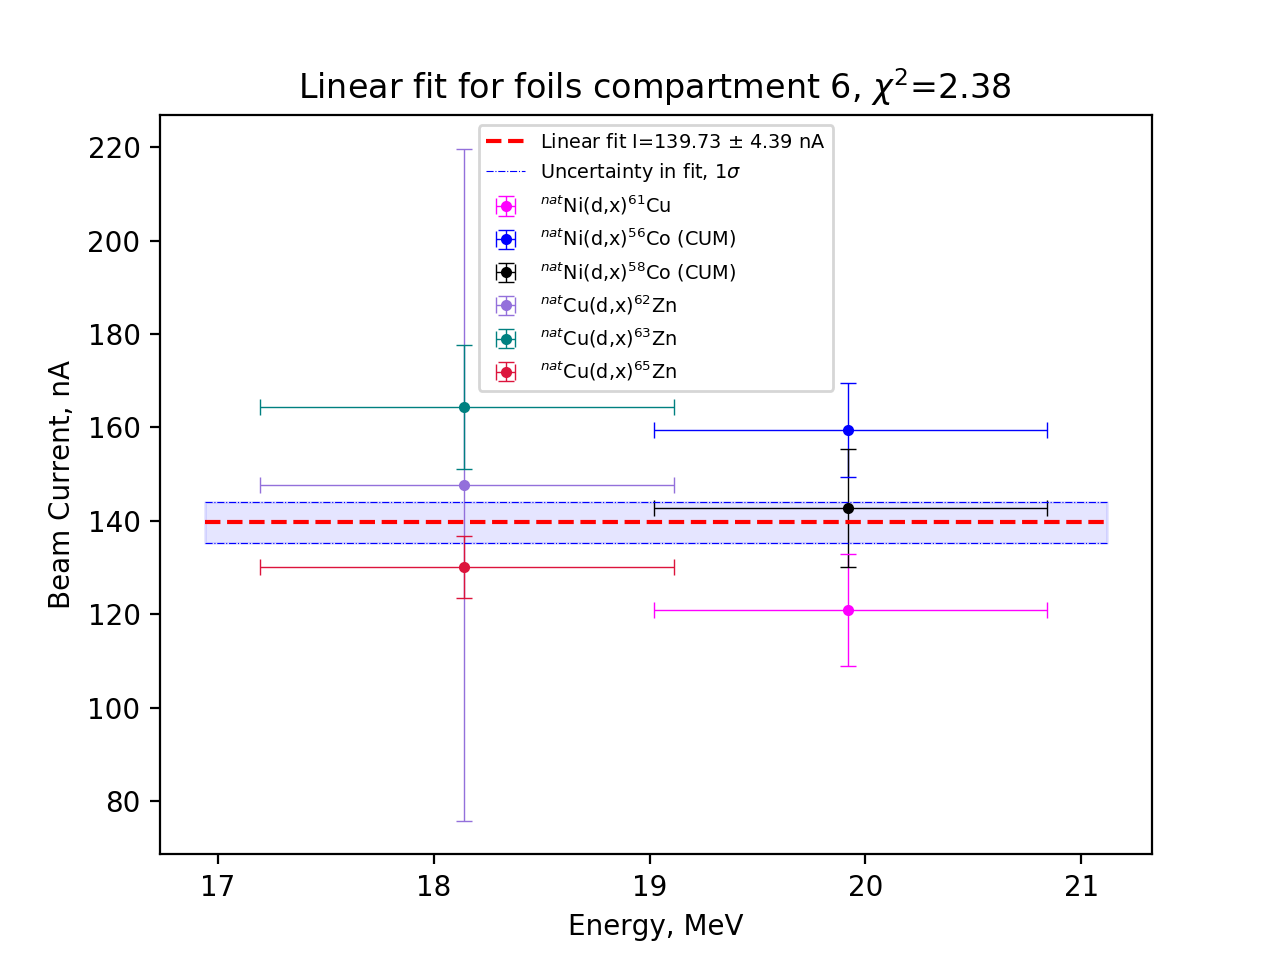
\includegraphics{Analysis/Compartment_6.png}
    \caption{The estimated (uncertainty weighted) beamcurrent over compartment 6.  }
    \label{fig:BC_comp6}
\end{figure}

\begin{figure}
    \centering
    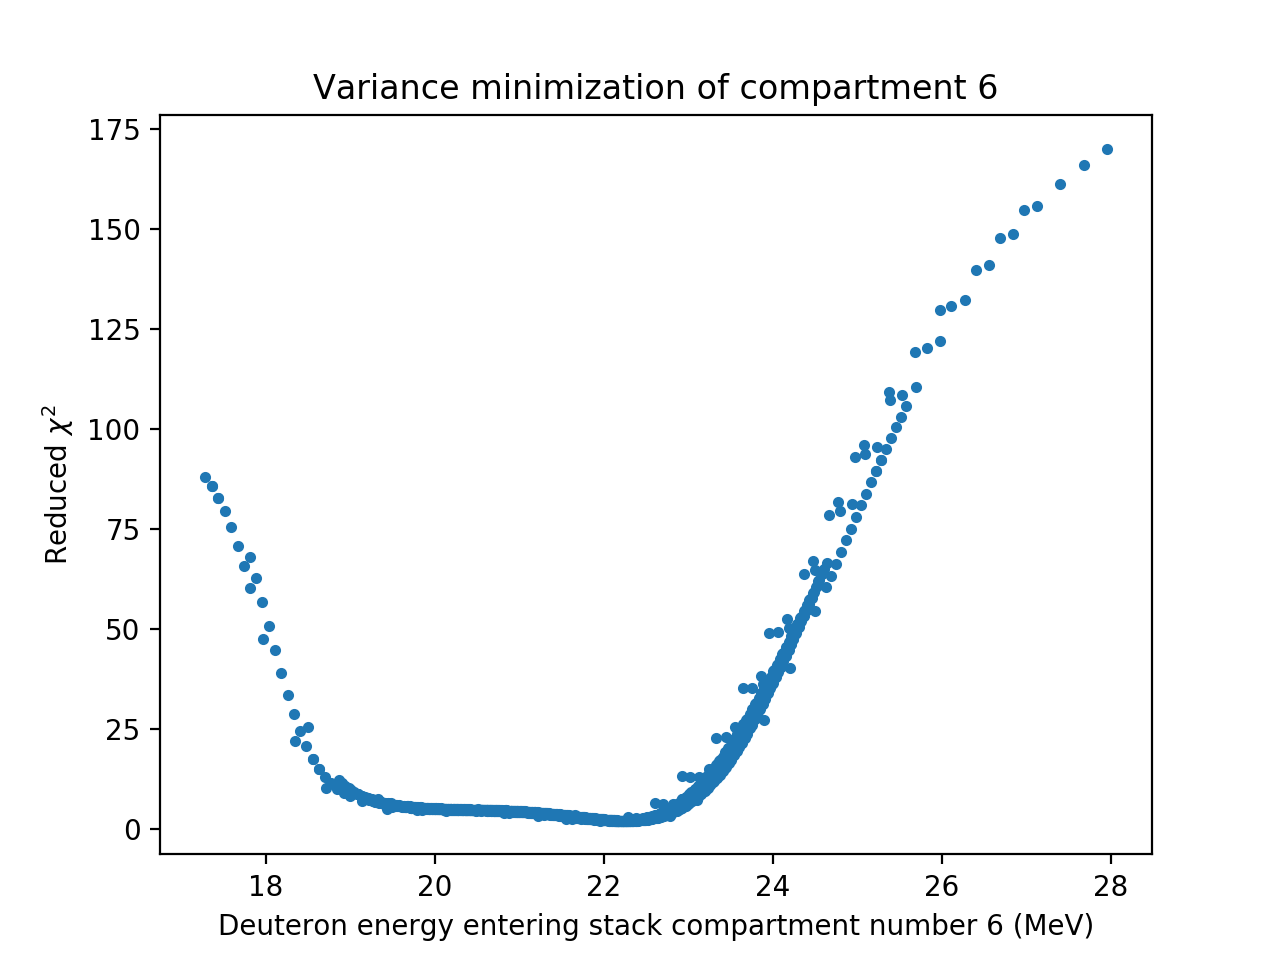
\includegraphics{Analysis/chisquared_comp6.png}
    \caption{The figure shows the estimated reduced $\chi^2$ as a function of the deuteron energy entering the stack (essensially the nickel flux weighted averaged beam energies).}
    \label{fig:chisq_curve}
\end{figure}

\noindent
Figure \ref{fig:varmin_beamcurrent} shows the beam current before (upper) and after variance minimization (lower), and the weighted average beam currents are listed in table \ref{tab:weighted_BC} estimated before and after the variance minimization. After variance minimization, the beam current estimated in each compartment (stabled lines) were similar, and meanwhile the weighted $\chi^2$ was about the same in compartment 6, it has improved in compartment 3 and very visible in compartment 9. In general the points are more aligned. $^{63}$Zn was constantly too high. The uncertainty in beam current is affected by the activity measured which again is affected by the counting statistics, the intensity of the gamma-lines used and uncertainty in the efficiency (figure \ref{fig:rel_uncertainty_efficiency}). Figure \ref{fig:rel_unc_BC} shows the relative uncertainty in beam current in each compartment using the flux weighted average beam energies of iridium, along with the relative uncertainty in each reaction. It shows that the uncertainty increases as a function of decreasing energy, which makes sense due to the uncertainty with the scattering processes taking place back in the stack. Yet a relative uncertainty of less than 5.5\% is ok. It is also clear that large uncertainties are weighted less than small uncertainties. Figure \ref{fig:monitor_BC} shows the estimated cross sections (estimated using equation \ref{eq:BC_simple}) where the estimated weighted average beam current for each target is plotted against the estimated cross section. In addition, the recommended IAEA cross sections \cite{Hermanne2018a} is plotted along with experimental data.


\pagestyle{empty}
\begin{figure}%
    \centering
    \subfloat{{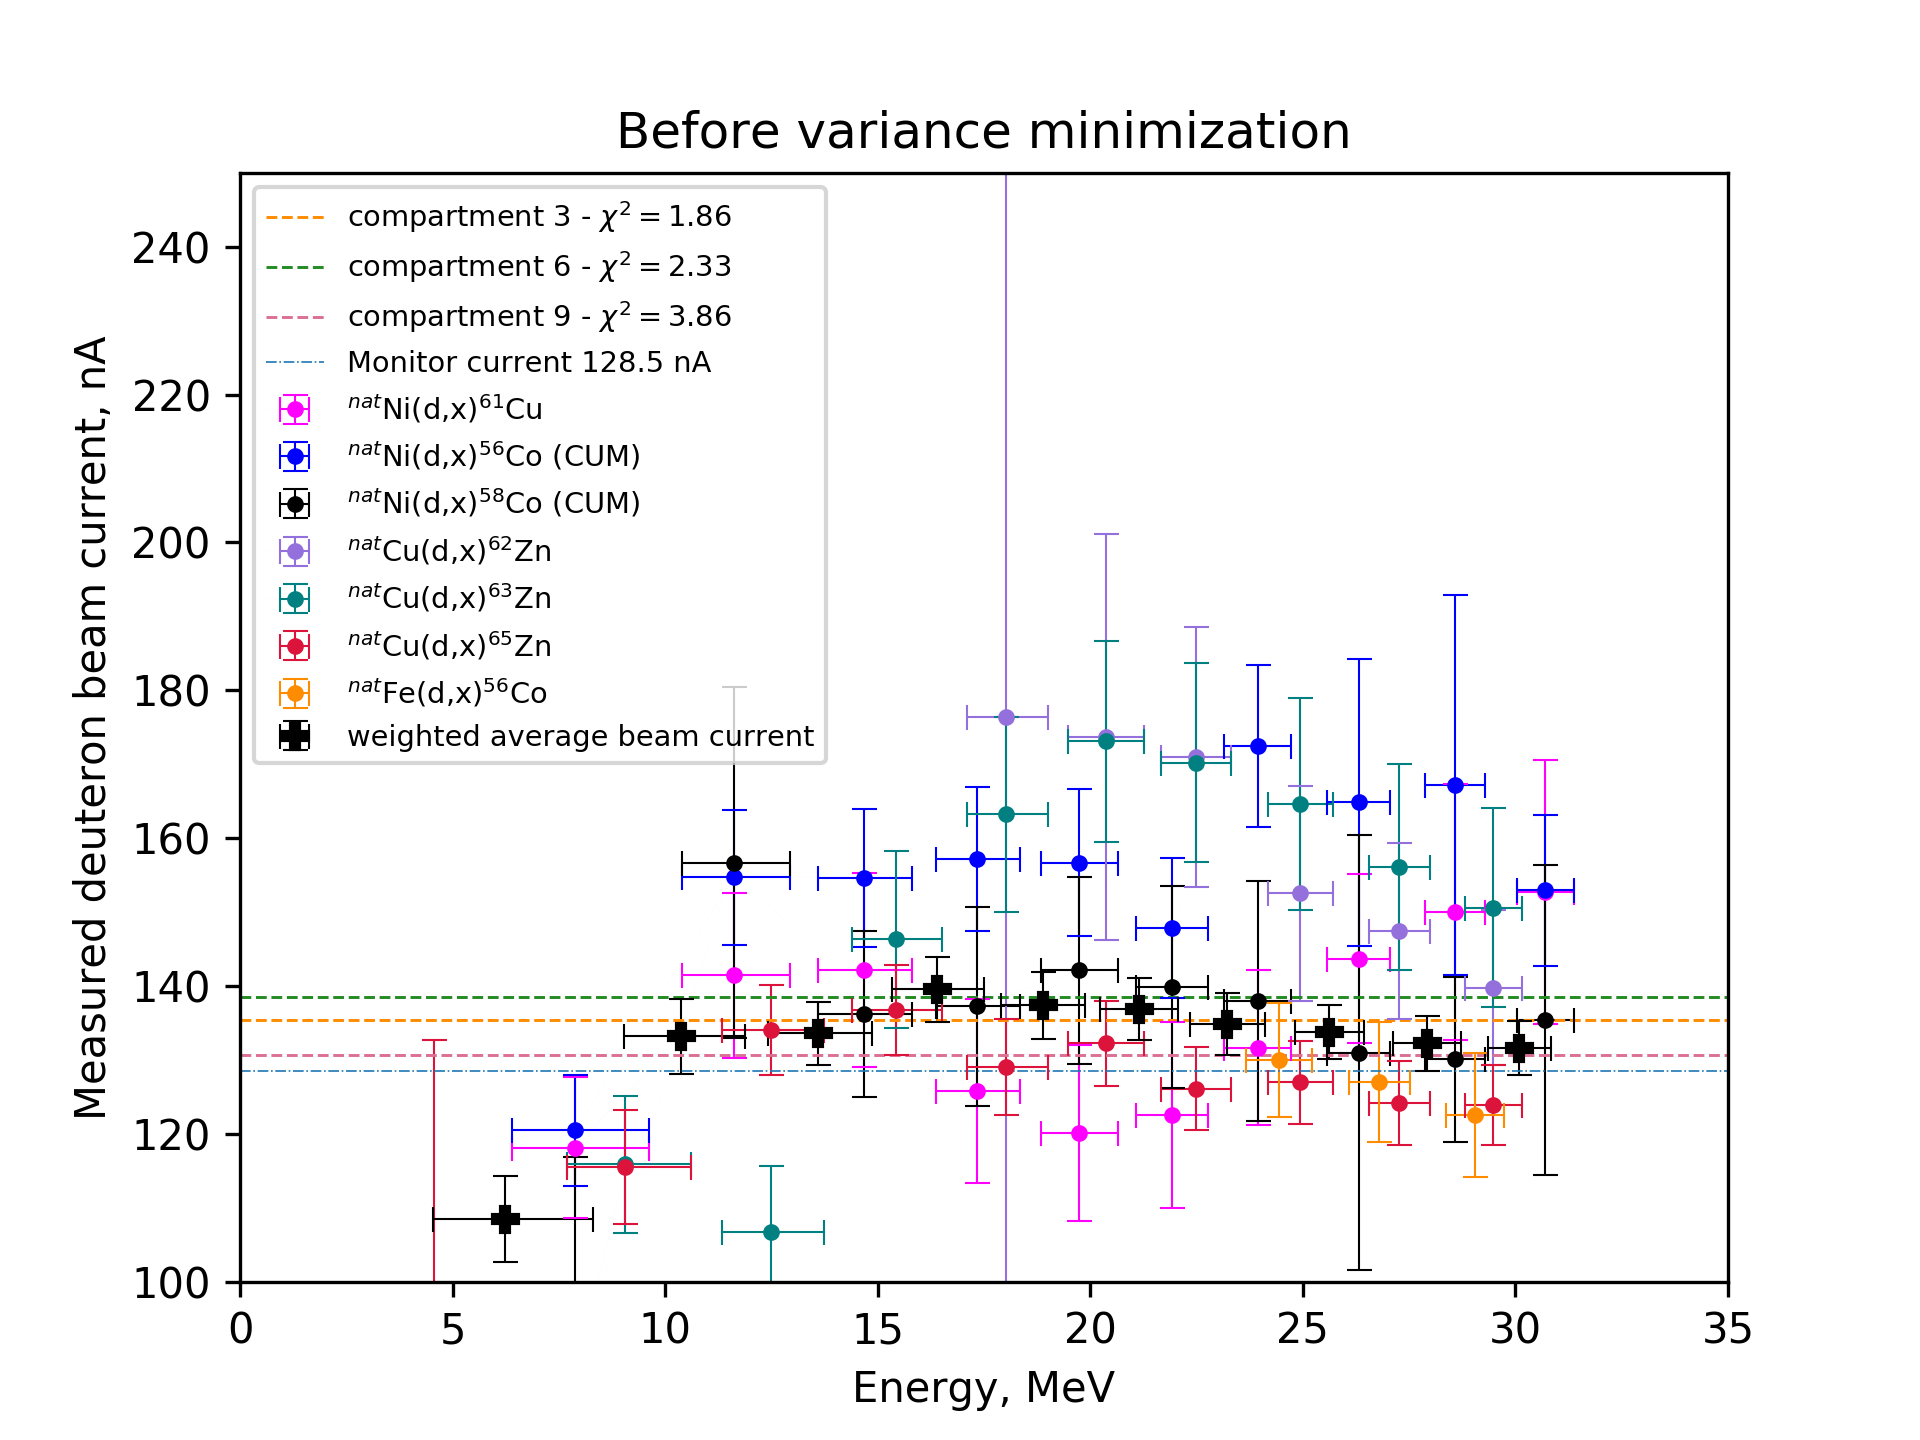
\includegraphics[width=17cm]{Analysis/beamcurrent_B_0_D_0.png} }}\hfill
    \subfloat{{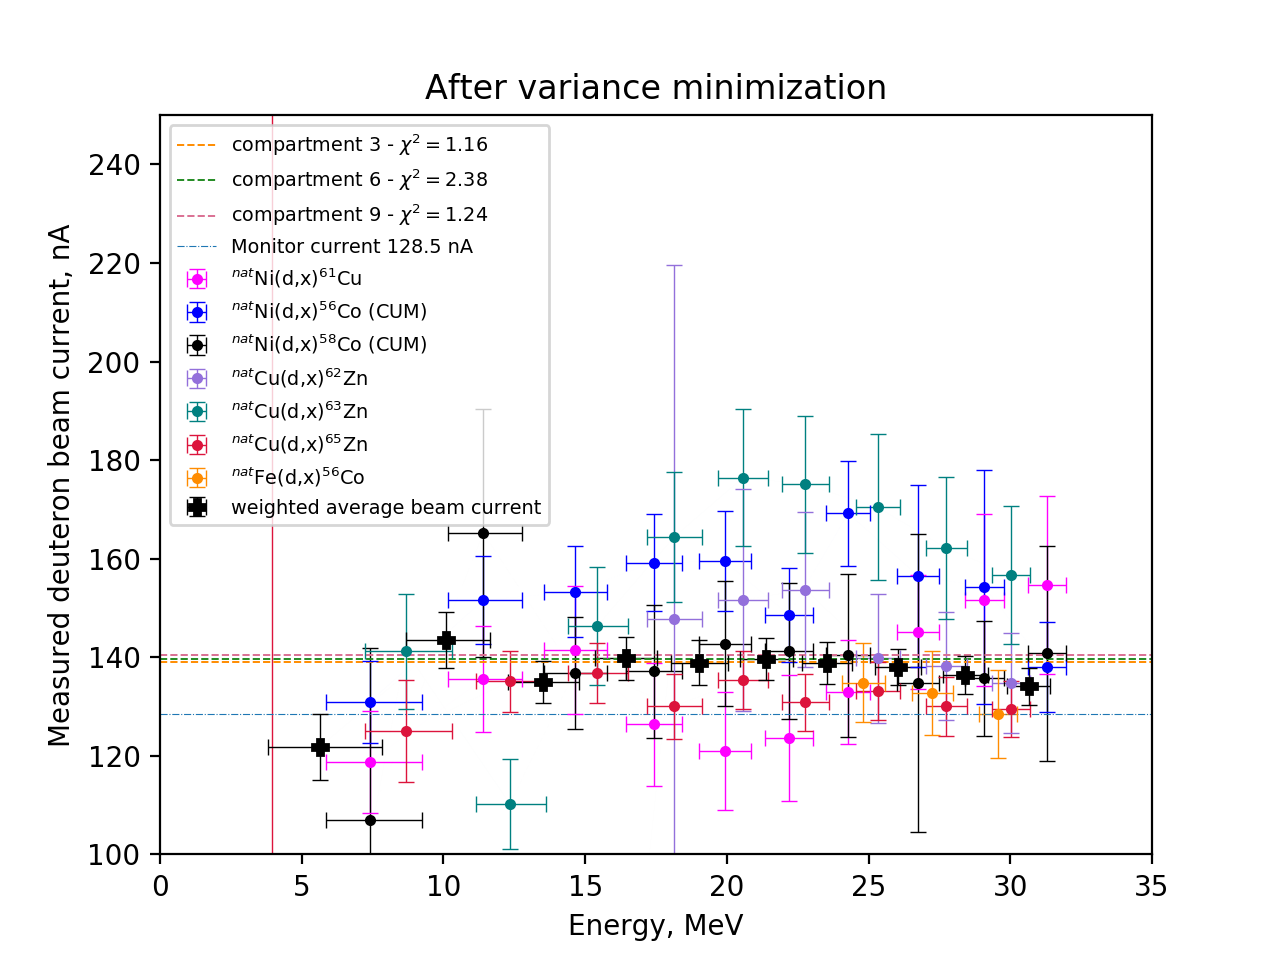
\includegraphics[width=17cm]{Analysis/beamcurrent_B_+2_D_+4,25.png} }}%
    \caption{Beam current before and after variance minimization. The final cross section was performed with a 2\% increase in beamcurrent and 4.25\% change in target foils. }%
    \label{fig:varmin_beamcurrent}%
\end{figure}

\begin{table}[]
    \centering
        \caption{The weighted average beam current before and after variance minimization in each compartment. The beam current on the 88-Inch Cyclotron beam integrator was 128.5 nA.}
    %\footnotesize
    \begin{tabular}{c |c c}
        \hline 
       Compartment & \makecell{Before} & \makecell{After}\\ 
        \hline 
        \makecell{01} & \makecell{131.56 \pm 3.64} & \makecell{134.08 \pm 3.70}  \\ 
        \makecell{02} & \makecell{132.23 \pm 3.74} & \makecell{136.42 \pm 3.83} \\ 
        \makecell{03} & \makecell{133.81 \pm 3.64 } & \makecell{138.02 \pm 3.75} \\ 
        \makecell{04} & \makecell{134.89 \pm 4.21 } &  \makecell{138.88 \pm 4.31}\\ 
        \makecell{05} &\makecell{136.85 \pm 4.21} & \makecell{139.67 \pm 4.29} \\
        \makecell{06} &\makecell{137.40 \pm 4.53} & \makecell{138.85 \pm 4.58} \\
        \makecell{07} &\makecell{139.55 \pm 4.37} & \makecell{139.77 \pm 4.37} \\
        \makecell{08} &\makecell{133.60 \pm 4.27} & \makecell{134.96 \pm 4.32}\\
        \makecell{09} &\makecell{133.16 \pm 5.04} & \makecell{143.59 \pm 5.67} \\
        \makecell{10} &\makecell{108.49 \pm 5.80} & \makecell{121.75 \pm 6.65} \\
    
         %\makecell{Before} & \makecell{131.56 \pm 3.64} & \makecell{132.23 \pm 3.74} & \makecell{133.81\pm3.64 } & \makecell{134.89\pm 4.21 } & \makecell{136.85_{\pm 4.21}} & \makecell{137.40 \pm 4.53} & \makecell{139.55 \pm 4.37} & \makecell{133.60 \pm 4.27} & \makecell{133.16 \pm 5.04} & \makecell{108.49 \pm 5.80}  \\
         %\makecell{After} & \\
    \end{tabular}
    \label{tab:weighted_BC}
\end{table}


\begin{figure}
    \centering
    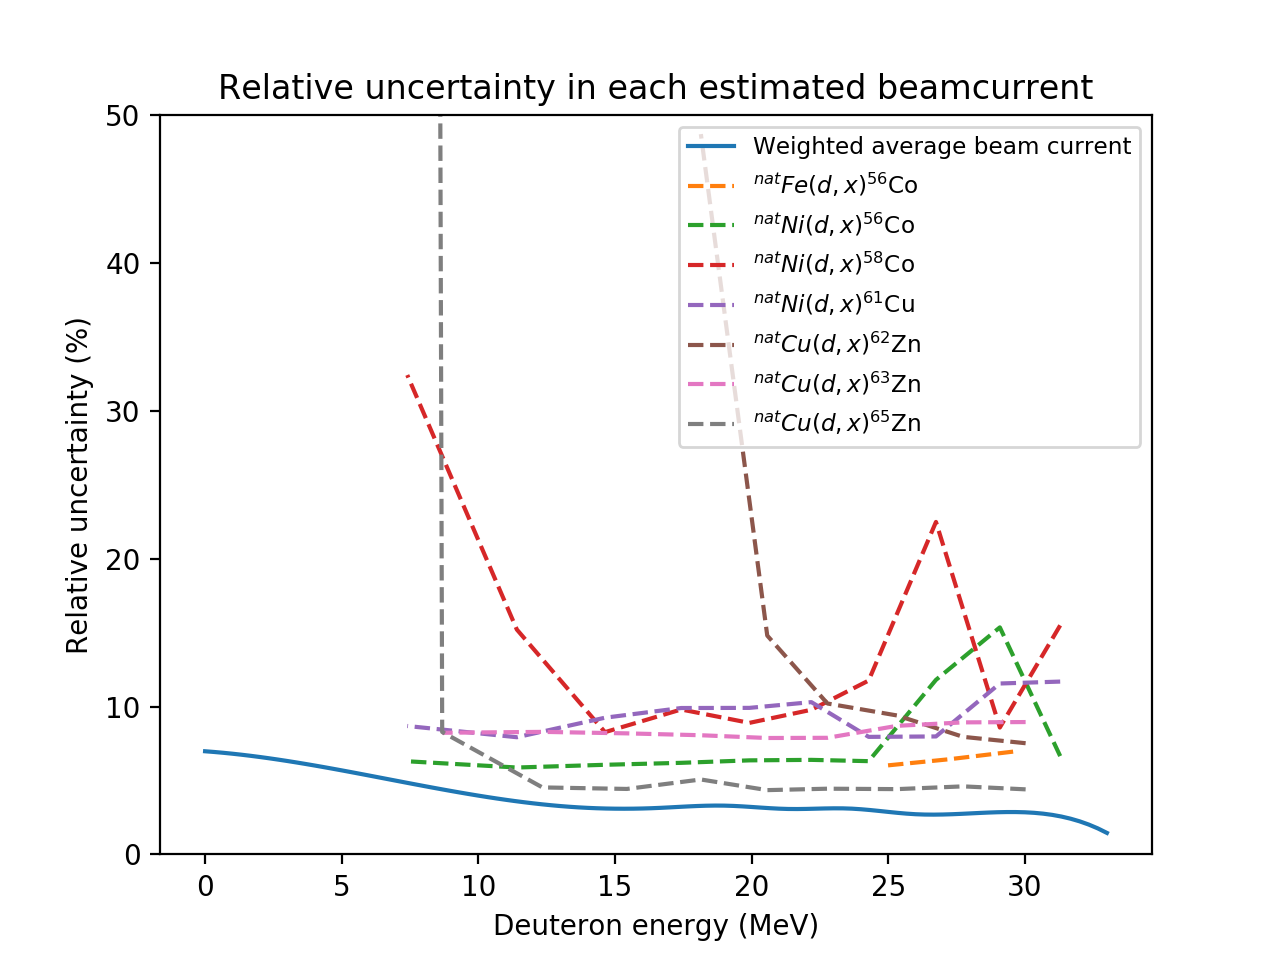
\includegraphics{Analysis/rel_unc_BC.png}
    \caption{The relative uncertainty in the weighted average beam current as a function of deuteron energy in each compartment. }
    \label{fig:rel_unc_BC}
\end{figure}


\begin{figure}%
    \centering
    \subfloat[]{{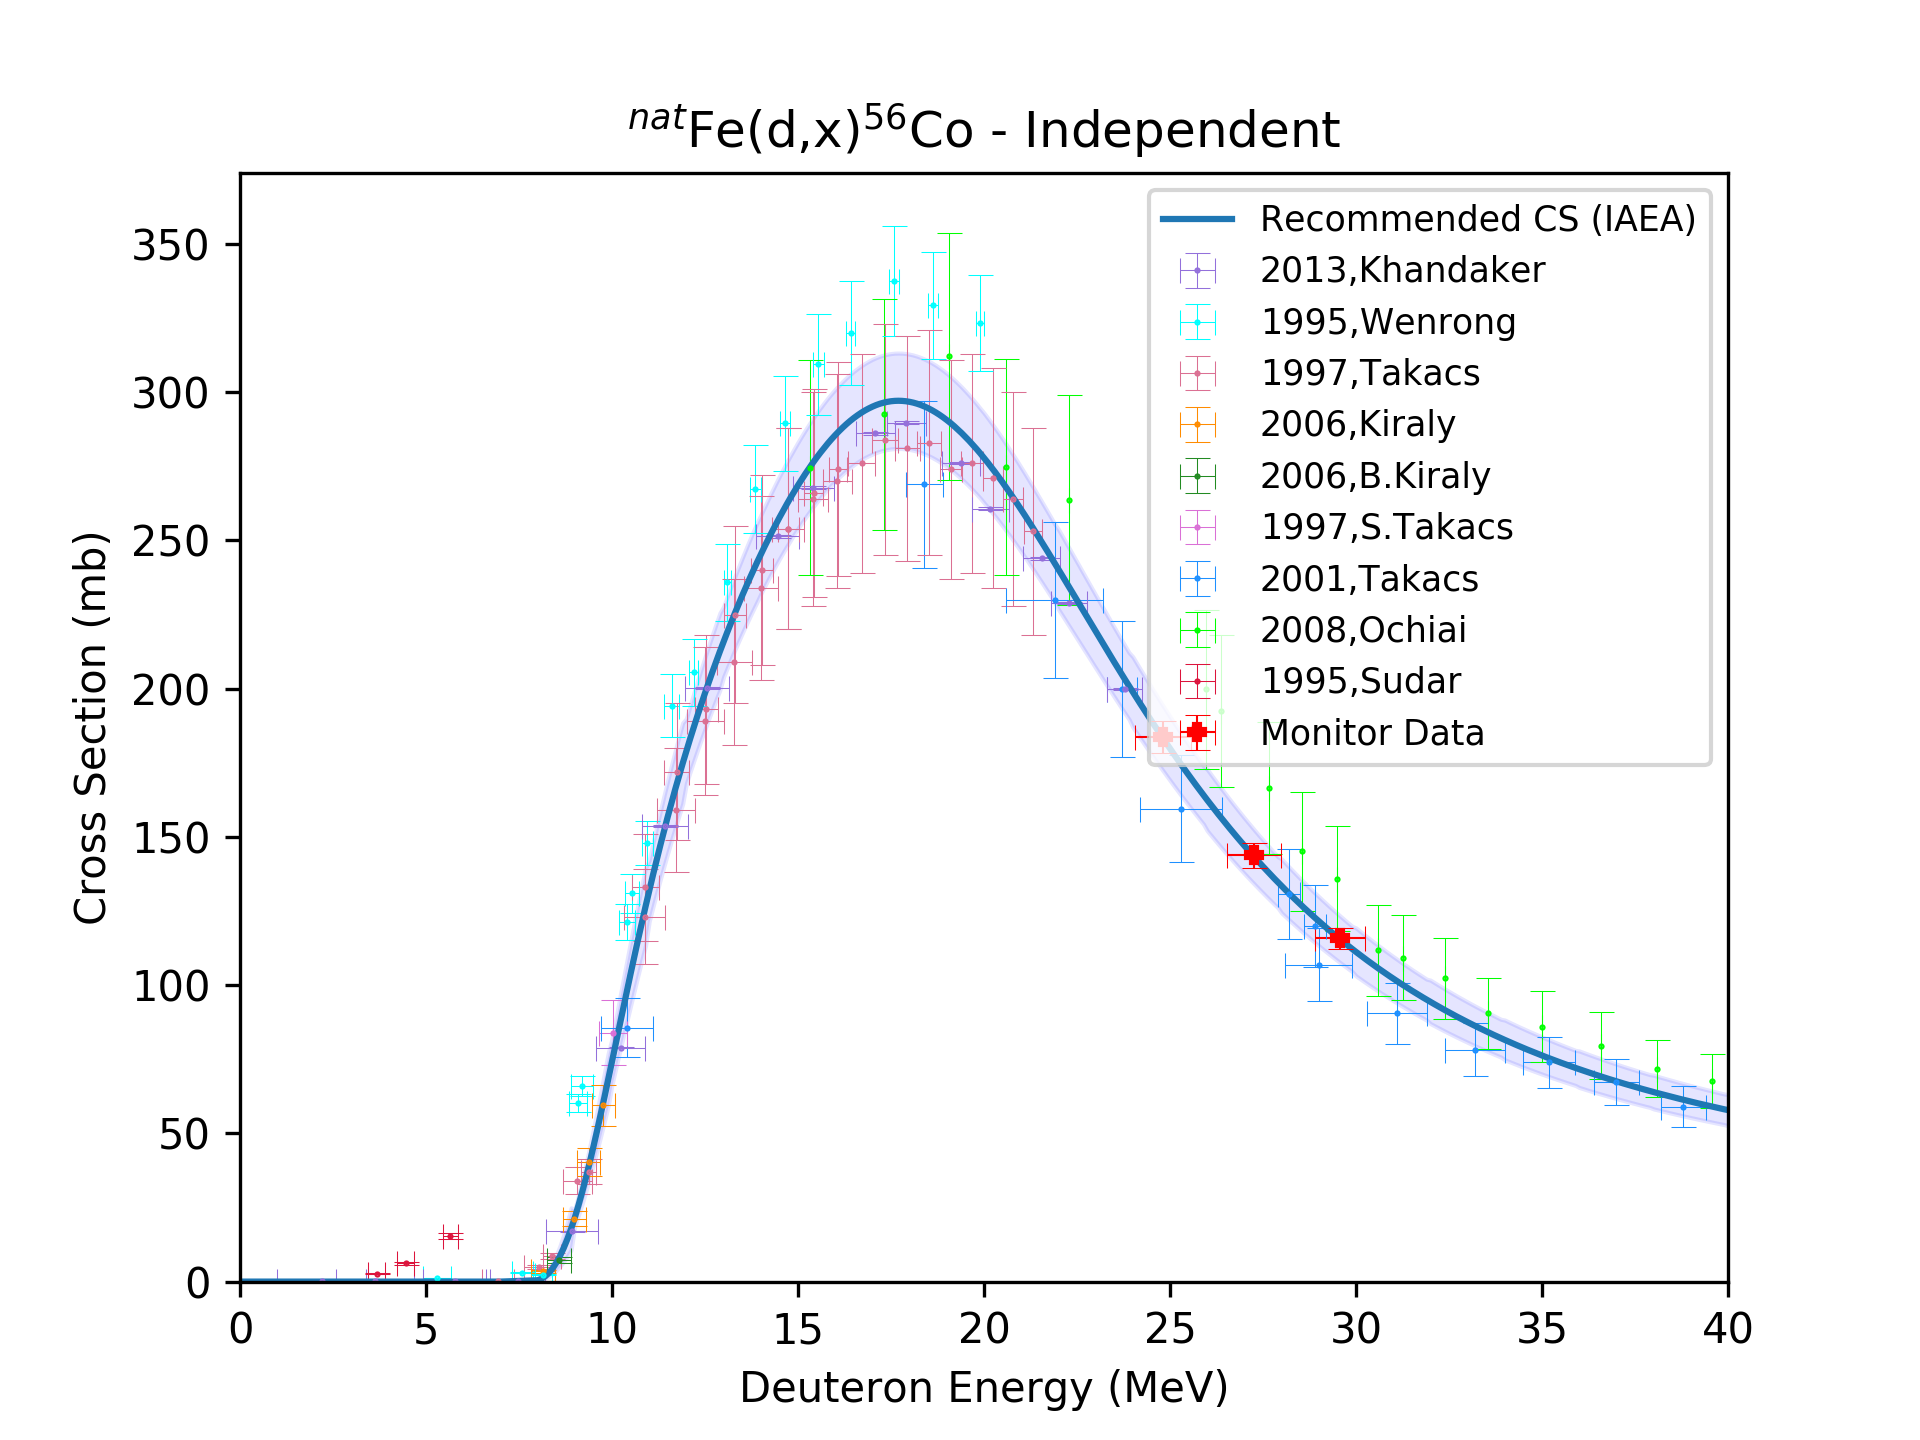
\includegraphics[width=7.5cm]{Analysis/Fe_56Co.png} }}%
    \quad
    \subfloat[]{{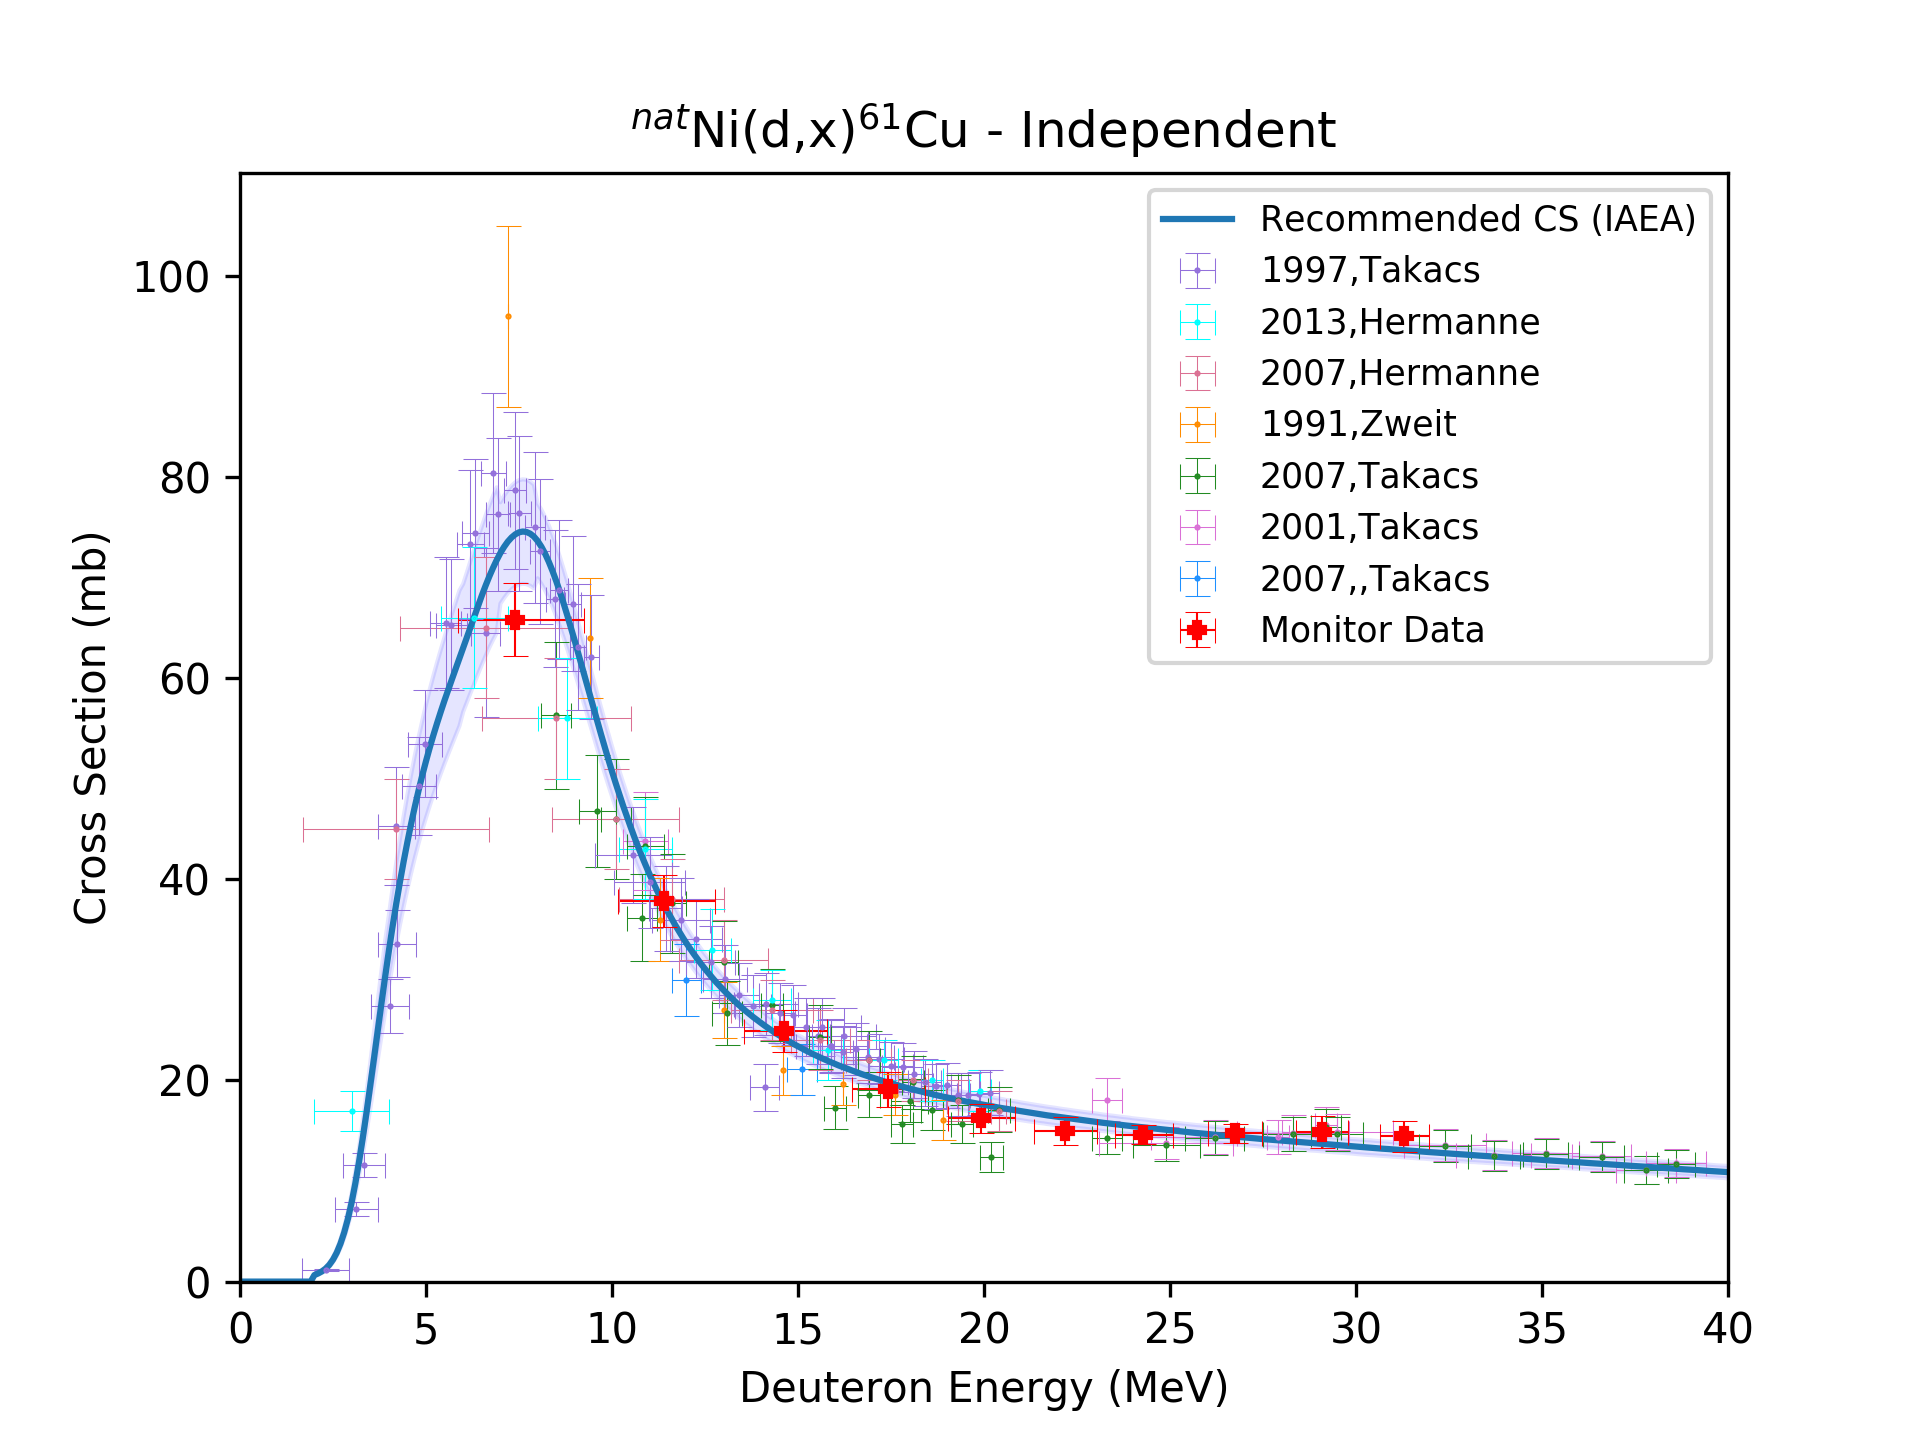
\includegraphics[width=7.5cm]{Analysis/Ni_61Cu.png} }}%
    \subfloat[]{{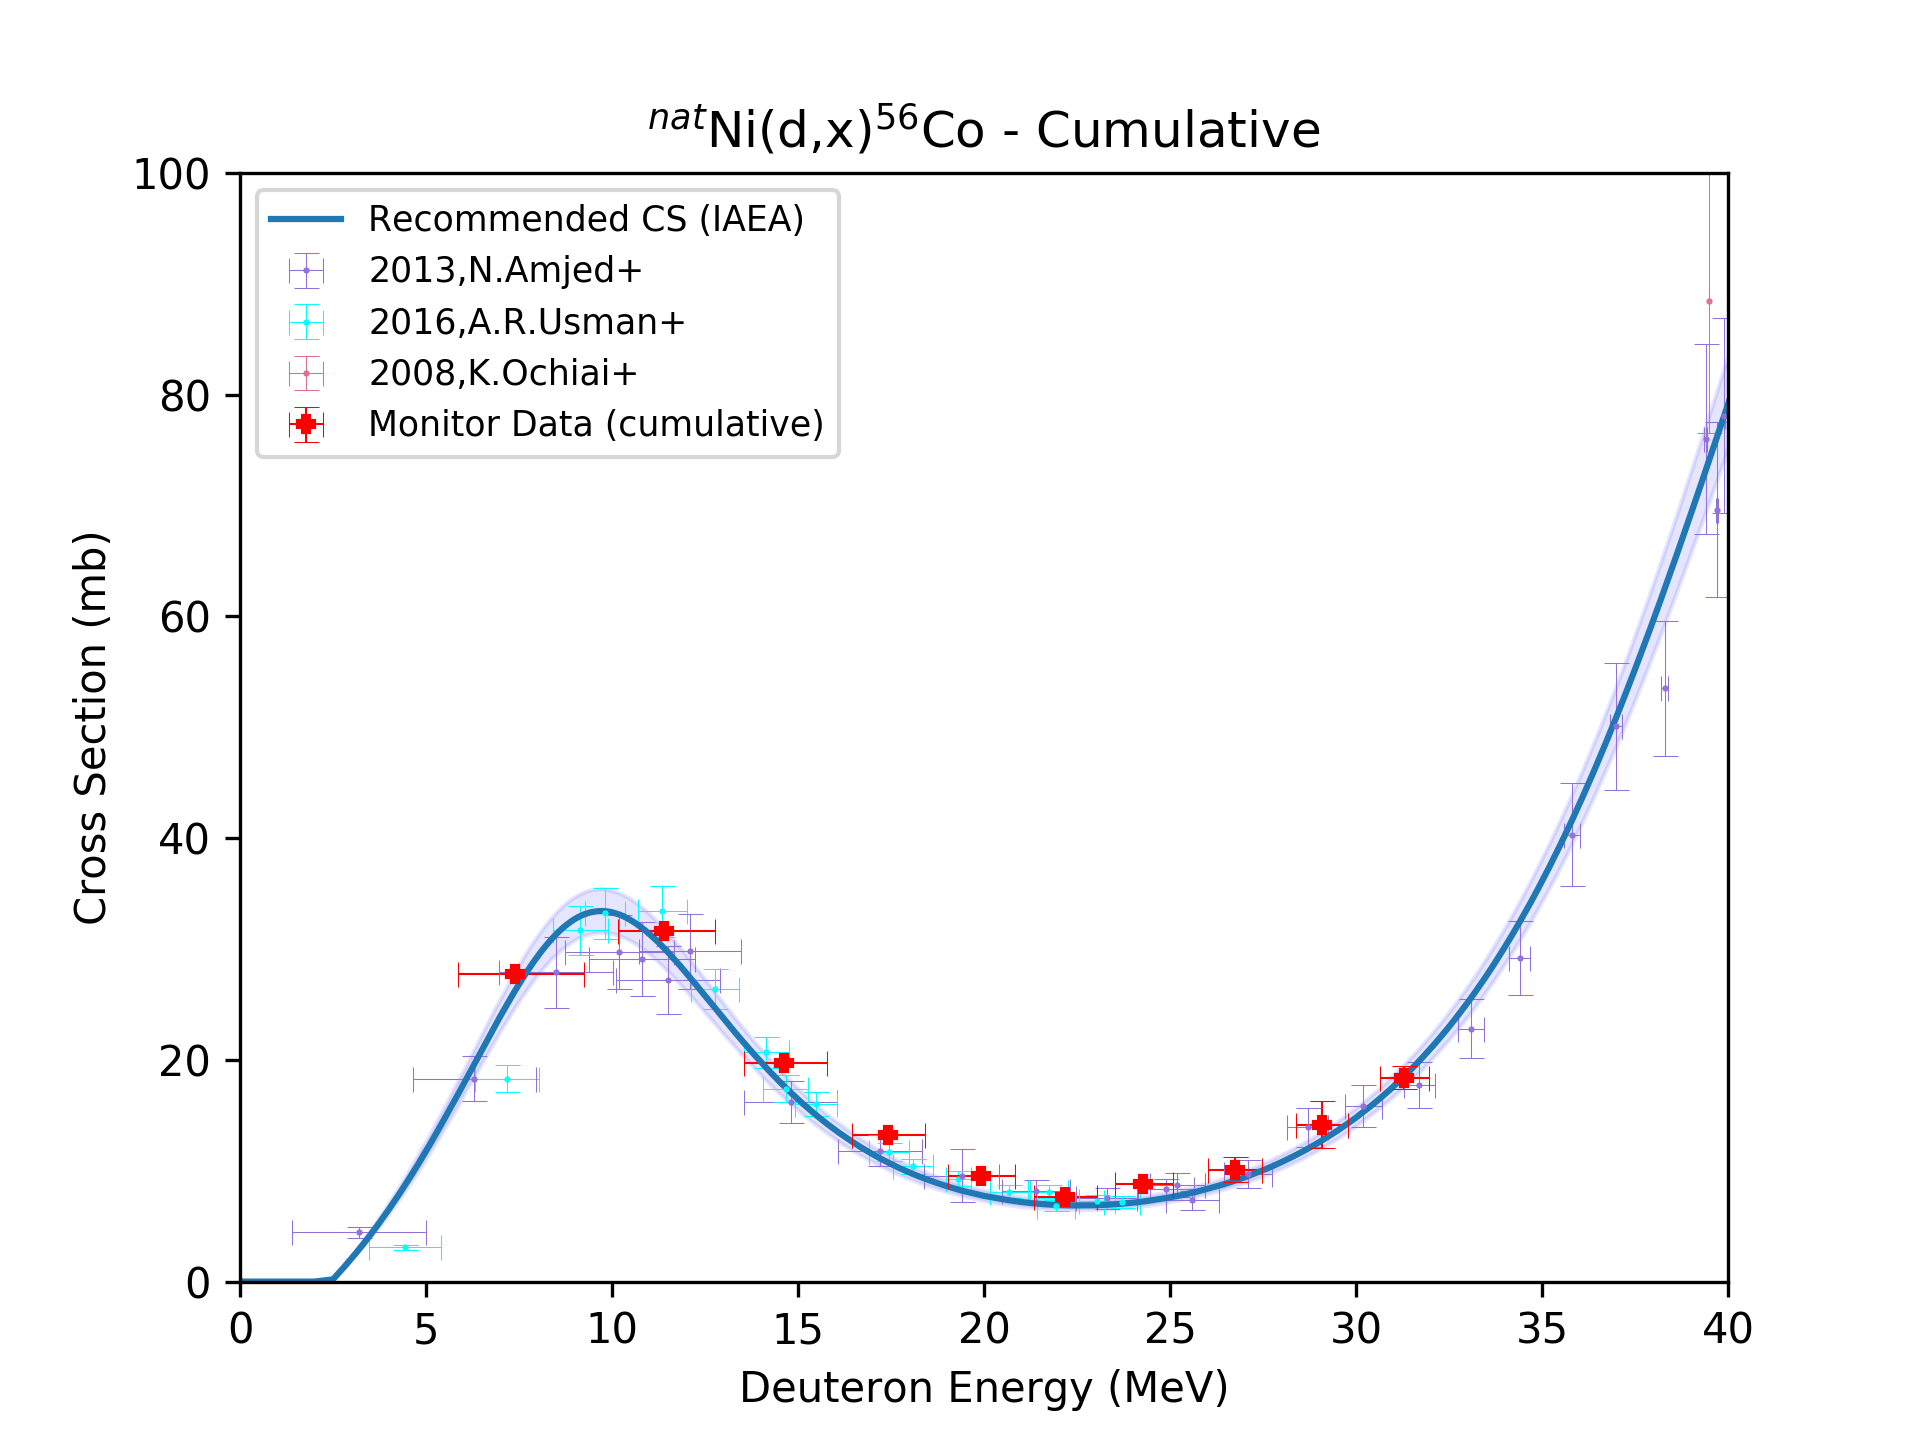
\includegraphics[width=7.5cm]{Analysis/Ni_56Co.png} }}%
    \quad
    \subfloat[]{{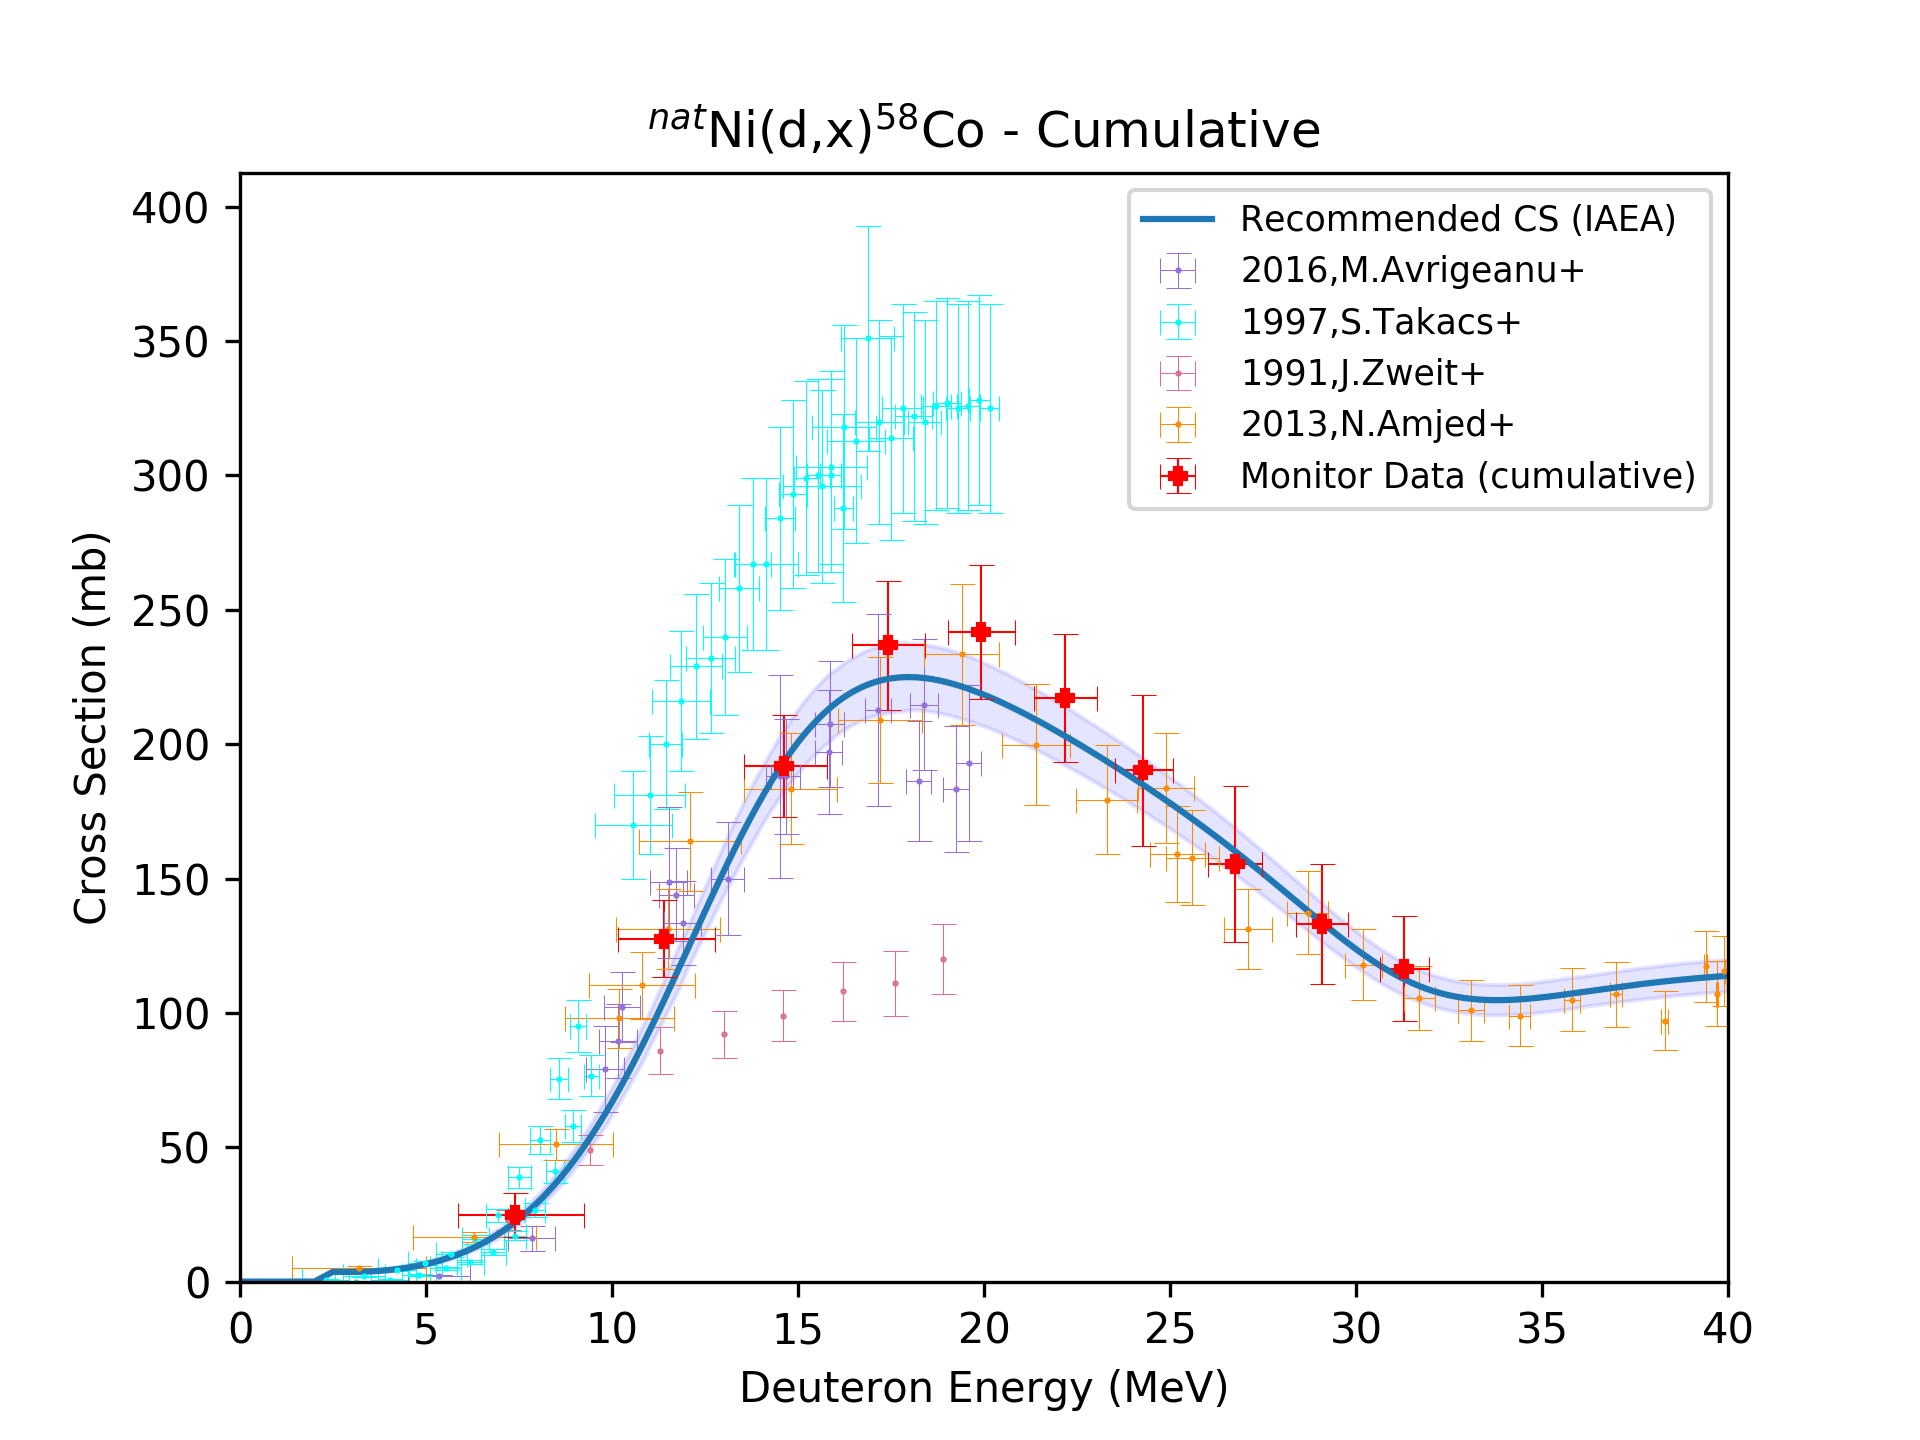
\includegraphics[width=7.5cm]{Analysis/Ni_58Co.png} }}%
    \quad
    \subfloat[caption]{{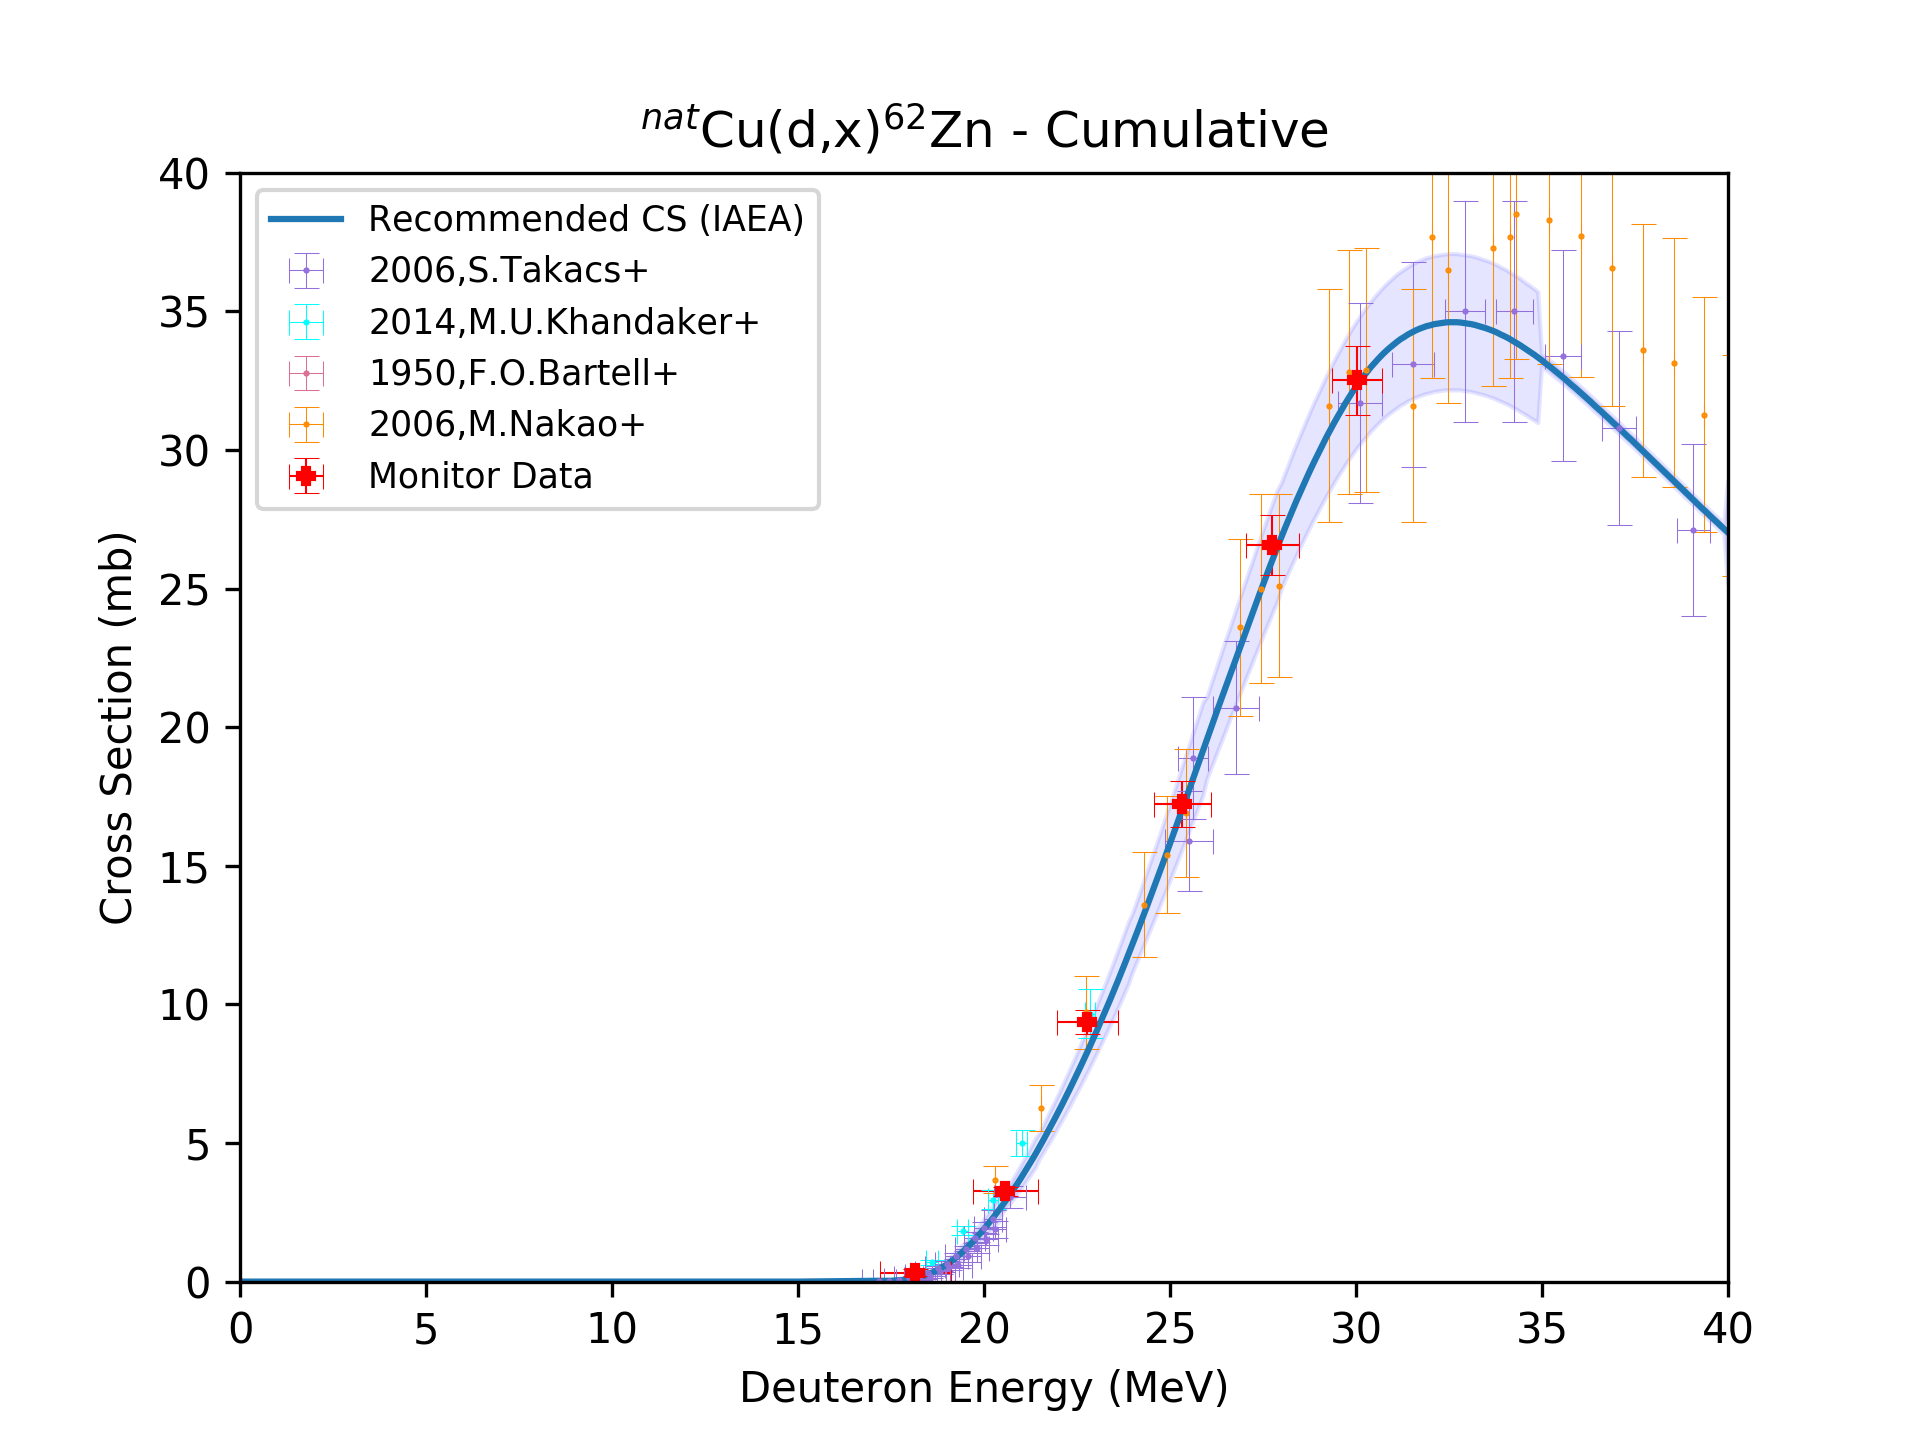
\includegraphics[width=7.5cm]{Analysis/Cu_62Zn.png} }}%
    \quad
    \subfloat[]{{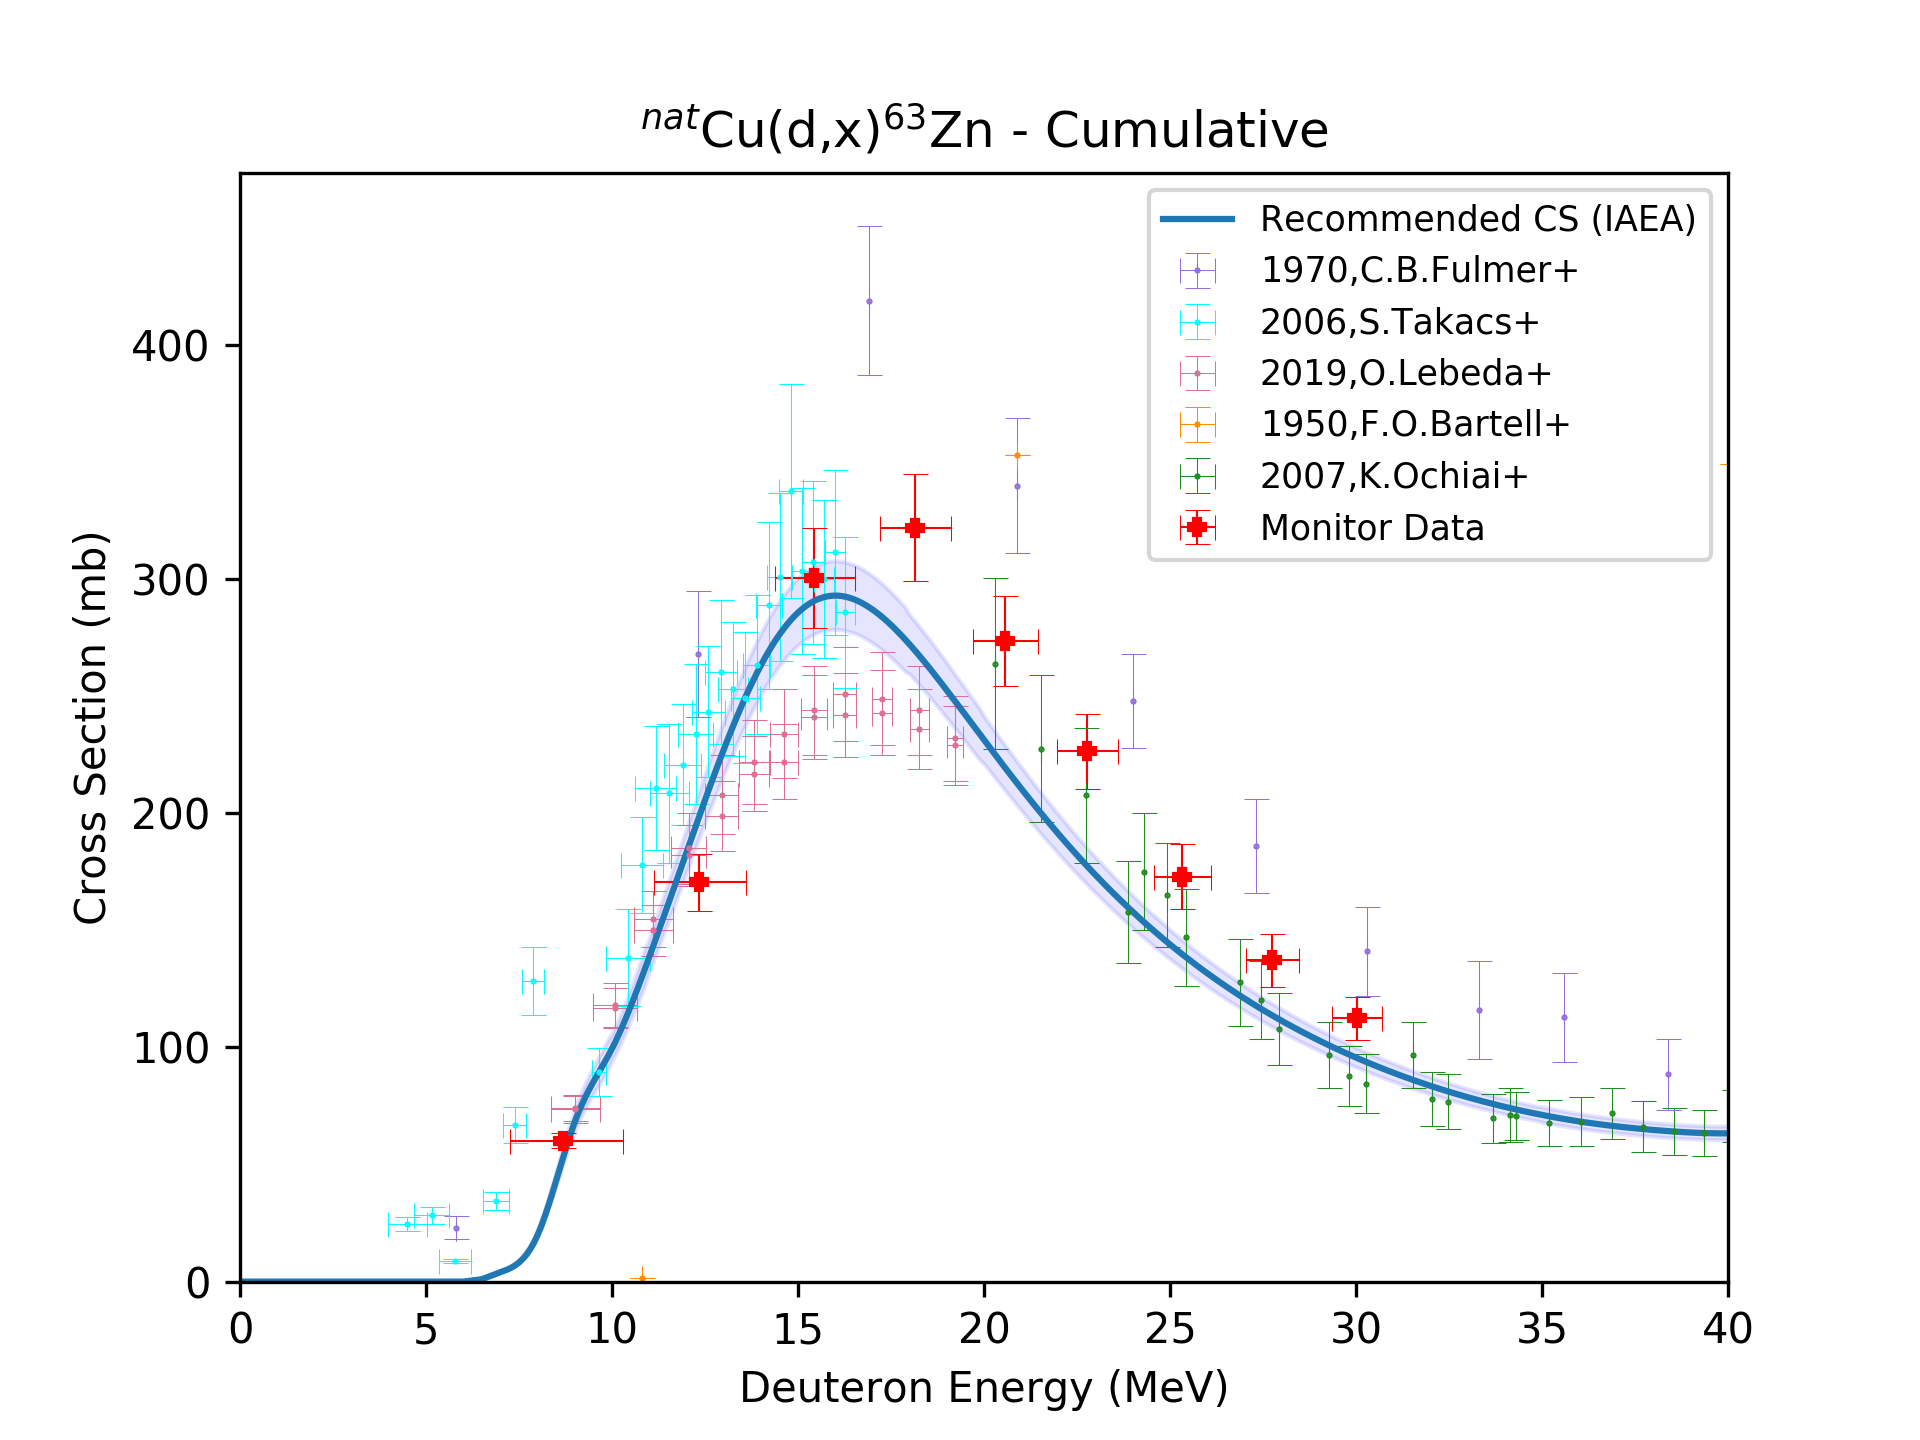
\includegraphics[width=7.5cm]{Analysis/Cu_63Zn.png} }}%
    \quad
    \subfloat[]{{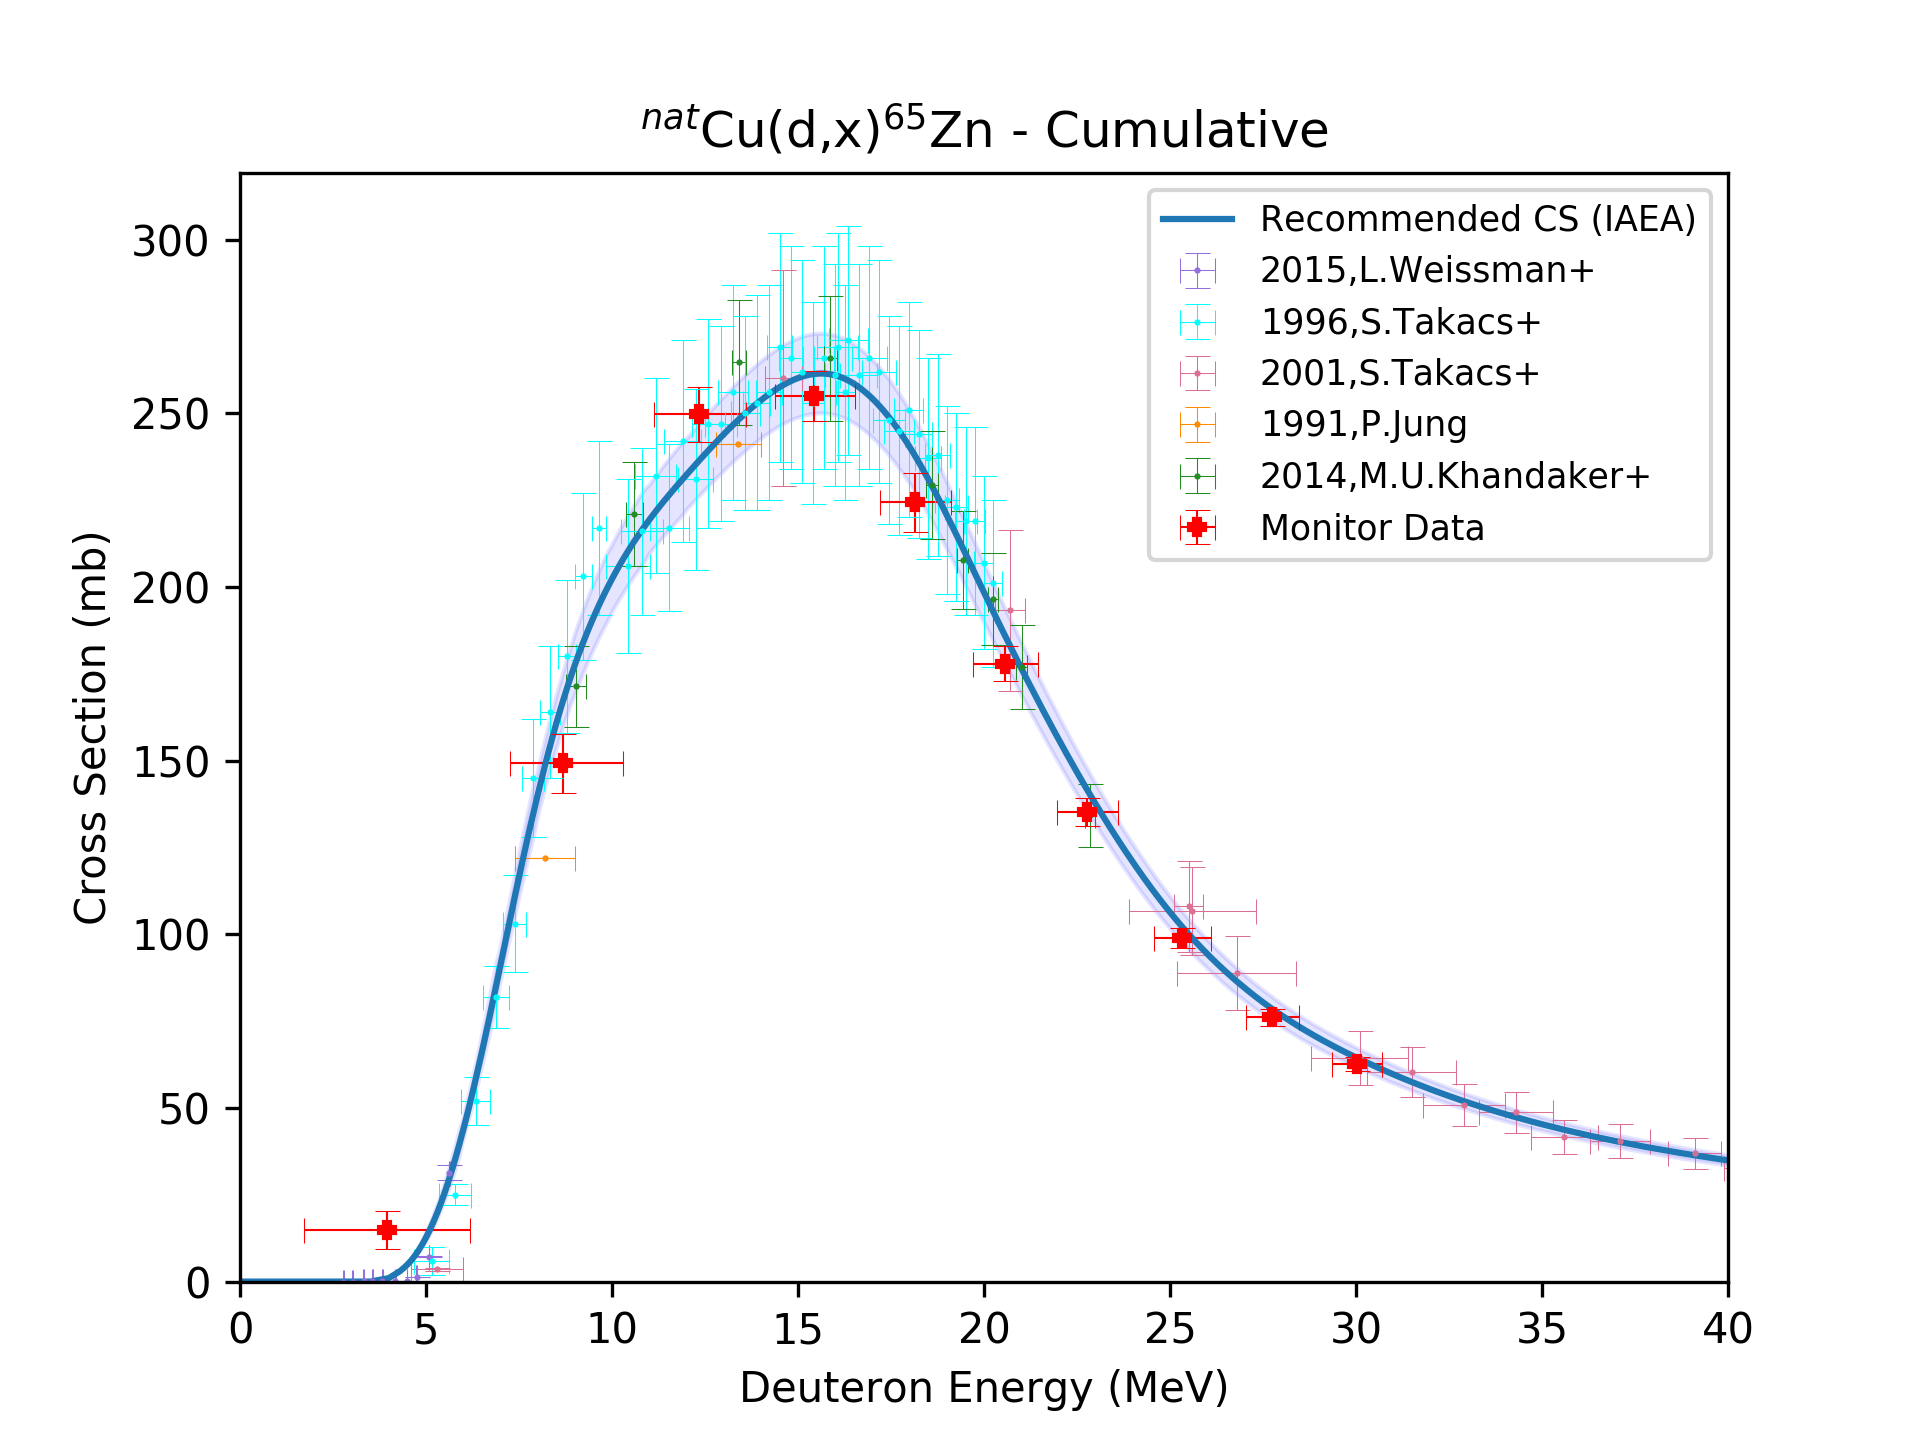
\includegraphics[width=7.5cm]{Analysis/Cu_65Zn.png} }}%
    \quad
    \caption{Figure shows the estimation of monitor cross section using the estimated weighted average beam current for each reaction (not the total). It is compared along with the recommended (IAEA) monitor data, and other experimental data  }%
    \label{fig:monitor_BC+CS}%
\end{figure}


\section{Cross sections}

The cross sections were finally calculated via equation \ref{eq:crossSection_simple}
\begin{equation}
    \sigma(E)=\frac{A_0}{\Phi(E)N_T(1-e^{-\lambda t_\text{irr}})}
\end{equation}

as a function of the weighted average beam energy,  the end of beamactivites for the product, the number of target nuclei, the weighted average beam current, the irradiation time and the decay constant of product. The cross section results are represented in the next chapter. Nuclei with beta- or isomer feeding were reported as cumulative, as well as the first observed element in a decay chain, due to the possible feeding from short-lived activities. The remaining activities which were not subject to feeding were reported as independent. Whenever it was possible to extract parent feeding from daughter activity (using the twostep decay), both the cumulative and independent cross sections are reported. In addition, if a parent nucleus with an independent cross section measurement feeds into a daughter nucleus, the total cumulative cross section measured in the daughter is

\begin{equation}
    \sigma_p*BR + \sigma_d = \sigma_{c}
\end{equation}

where BR is the branching ratio of the feeding from the parent nucleus. The independent daughter cross section was thus estimated by subtracting the total cumulative cross section and the cross section from the parent cross section. Likewise, if two independent cross sections of daughter and parent were observed, the cumulative is reported by adding together. 


\\

\noindent 
The measured data is compared to previous experimental data from the EXFOR-database, along with nuclear reactor models TALYS-1.9, TENDL-2019, ALICE-2017\cite{Blann1996}, CoH-3.5.3 and EMPIRE.... The theoretical models are important for several reasons, the general understanding of the reaction (\cite{international2012iaea}, p. 23), and it can help to build confidence in experimental data. The default parameters for each reaction was used, so there was no change to the nuclear structure or the modeling of the reaction physics. Tuning the function will improve the local optimization, but it will not contribute to improving the code globally. Since the majority of the cross section measurements compares to the reaction models using default parameters, this is also what have been done in this work. The use of default parameters also reveals how well the code predicts the excitation function (\textcolor{red}{citation, comments from Andrew}). The exception was for CoH deuterons on iridium, for the exit channels alpha-particles and neutrons. The parameter \textit{tweakSD} was set to 0.25 which adjusts the effective single-particle state density\footnote{http://physics.ucsc.edu/~peter/112/dos.pdf}. A 25\% change of the single-particle state density for outgoing alpha-particles and neutrons is a huge change, but had to be done to get it to work. \\

\footnote{https://doi.org/10.1016/j.nds.2012.11.002}: Talys is a model for nuclear reactions involving neutrons, $^3$He, protons, photons, deuterons, trirons, alphaparticles in the 1 keV-200 MeV range for target nuclides of mass 5 and heavier. 
OPTICAL MODEL: represents the complicacted interaction between an incident particle and a nucleus by a complex mean-field potential, which divides the reaction flux into a part covering shape elastic scattering and a part describing all the competing reaction channels. The input parameters; projectile, element, mass (natural) and the energy! 

For compound nuclear reactions, the optical model, level density, gamma-ray strength function and fission transmissions coefficient as ingridients, low energy reactions. Both capture of the projectile and the multiple emission chain for the excited residual nuclides are needed. 


%ALICE-2017 is a precompound Monte Carlo simulation, where the number of target nuclei was ..., ... ,, 








Here write a few sentences about how each was done and the motivation behind it. 





\begin{comment}
%The analysis of estimating production cross sections consisted of multiple steps. To obtain the end of beam activities the peak areas (number of counts) were found with gamma-ray spectroscopy using FitzPeaks\footnote{https://www.jimfitz.co.uk/fitzpeak.htm}. The efficiency calibration as a function of gammaray energy was done using $^{137}$Cs, $^{133}$Ba and $^{152}$Eu point sources. The energy degradation in the foils were simulated using NPAT\footnote{https://pypi.org/project/npat/}, giving the deuteron flux as a function of energy. Along with the simulation and IAEA recommened cross sections for the monitor reactions\footnote{https://www-nds.iaea.org/medical/monitor_reactions.html}, the weighted average beam current was estimated in each foil. 

%\section{Gamma-ray spectroscopy}
%The spectra were analyzed in FitzPeakz\footnote{https://www.jimfitz.co.uk/fitzpeak.htm}. The mathematic algorithm in which FitzPeakz is based upon is SAMPO80 \footnote{https://sci-hub.tw/https://doi.org/10.1016/0029-554X(81)90209-3}. \textcolor{blue}{The peaks are assumed Gaussian with an exponential tale on both sides of the peak. The exponential tale and Gaussian function are joined so function and first derivative are continous. The algorithm searches for peaks by using the smooth second difference (derivative?) Particularly good for detecting small peaks on a high or low background. The peak areas are calculated by fitting the precalibrated modified Gaussian to the data with a weighted least squares formula using a parabolic background. Fitting intervals are determined automatically by the program. Peaks separarated by less than 4 times the average fwhm are fitted together. }

%For each spectra,  a report file containing peak energy, centre channel, full width half maximum, significance, goodness of fit, peak area, uncertainty in peak area, gammas per second, uncertainty in gammas per second and a background estimation for each peak was provided. The most important parameters were the energy, the peak area $N_C$ and uncertainty in peak area. Peak area was needed for the activity calculation in equation \ref{eq:Final_Expression_A0} which is an important parameter in the calculation of the cross section (equation \ref{eq:experimental_CS}), and in the calculation of the efficiency for the calibration sources (equation \ref{eq:efficiency_analytical}). Gammas per second (also called countrate) was used to get an indication if the rate of gammas, which were used as a critical tool to evaluate background contamination in a peak for instance. 


%\subsection{Energy and peak-shape calibration} \label{subsec:fitz_calibration}
%Used calibration sources $^{137}$Cs ($t_{1/2}=30.08$ years\cite{Browne2007}), $^{133}$Ba ($t_{1/2}=10.551$ years\cite{Khazov2011}) and $^{152}$Eu ($t_{1/2}=13.517$ years\cite{Martin2013}), which can be seen on figure \ref{fig:calsources}.

%\textcolor{blue}{The calculated peak locations and areas are finally corrected with energy and efficiency calibration data to yield peak energies and intensities. For the energy calibration, linear interpolation on a linear scale and for the efficiency calibration linear interpolation on a log-log scale are used in this code. Calibration errors are added to the peak location and intensity errors to give the final result (p.94). \\ The peak shape calibration uses 7 parameters; two background peaks, peak height and location, peak width, distance from peak centroid to the starting point of exponential on either side. The minimization of the least-squares expression to solve for the peak parameters is done by a subroutine package  with an iterative gradient algorithm utilizing the variable metric method. Minimization is terminated when all all components in the next step change by less than $10^{-8}$, if four succeeding values of $\chi^2$ are the same or if 100 iterations have been completed. The performed shape calibration can be checked with a few parameters, goodness of fit, $\chi^2$ per degree of freedom, sigma and error correlation. Sigma below 5 and error correlation between -1 and 1 are acceptable values.  (p.90)} \\


%From the webpage\foonote{jim-fitz.com/calib.html}:
%Each detector was calibrated with peak shape and energy for the calibration sources. Fitzpeakz takes in energy (.enc) and peak shape (.shp) calibration source files, containing the energies listed in table\ref{table:calibration_gammas}. For the peak shape, the program determines the parameters of width and the amount of low energy tailing. The energy calibration and peak shape calibration was estimated to a 1st order function. 

%\subsection{Background subtraction}

$How it was done very simple!!

%\section{Efficiency calibration} \label{sec:efficiency_calibration}
%The efficiency calibration is an important factor in the calculation of the cross section in equation \ref{eq:experimental_CS}. The detector efficiency is the number of events registered divided by the events emitted by the source. The absolute efficiency can be divided into intrinsic and geometrical efficiency, where the intrinsic efficiency is the number of events registered divided by the number of events hitting the detector. The
%intrinsic efficiency thus depends on the interaction cross section between incident particle and detector material. For neutral particles, the size of the detector affects the intrinsic efficiency, the larger crystal the larger the probability of interaction is. The geometrical efficiency is the radiation emitted by the source which hits the detector. (Techniques for Nuclear and Particle Physics Experiments. William R. Leo. Second Revised Edition. Springer.Verlag Berkling Heidelberg GmbH, New York (1994). p. 121-122 ) \\

%\noindent 
%The efficiency was measured using calibration point sources $^{137}$Cs ($t_{1/2}=30.08$ years\cite{Browne2007}), $^{133}$Ba ($t_{1/2}=10.551$ years\cite{Khazov2011}) and $^{152}$Eu ($t_{1/2}=13.517$ years\cite{Martin2013}). Figure \ref{fig:calsources} shows the calibration points sources ($^{22}$Na was excluded during the data-analysis since it only contains a single gamma-line and gave poorer results). On each calibration source, a reference date is given with an activity, which here is referenced to as $A_0$ of the calibration sources.\\

%\noindent Solving Equation \ref{eq:Final_Expression_A0} for effiency, $\epsilon$, the analytical effiency as a function of gamma-ray energy and intensity is 
%\begin{equation} \label{eq:efficiency_analytical}
%    \epsilon(E_\gamma)= \frac{N_C \lambda}{A_0 I_\gamma (1-e^{-\lambda \Delta t_c})e^{-\lambda\Delta t_d}}
%\end{equation}

where $\lambda$ is the decay constant and $N_C$ is the number of counts in the measured spectra, and $\Delta t_d$ is the delay time since the reference date. The analytical efficiency gives one single value for the efficiency at energy $E_\gamma$, but we want a continuous function which gives the effciency at any gamma-energy. A model based upon Gallagher, W. J., Cipolla, S.J. (1974) was applied which takes the probability of penetration through the deadlayer of the detector and the probability of interaction in the detector volume into account

\begin{equation} \label{eq:efficiency_estimated}
\epsilon(E_\gamma) =  B_0 + \underbrace{(e^{-B_1 E_\gamma^{B_2}})}_\text{dead layer}  \underbrace{(1-e^{-B_3 E_\gamma^{B_4}}))}_\text{interacting with volume} 
\end{equation}
\noindent 
where $B_i$ is optimum parameters minimizing the $\chi^2$ in the scipy optimizing curve fit function\footnote{https://docs.scipy.org/doc/scipy/reference/generated/scipy.optimize.curve_fit.html}). Figure \ref{fig:efficiency_curve} shows an example of an efficiency curve for a detector at a specific distance from the detector. The uncertainty of the efficiency was estimated using equation \ref{eq:variance_full} numerically. For each source, the gamma-lines with the intensities which were used to calculate the efficiency points for each source is listed in table \ref{table:calibration_gammas}. \\


\begin{figure}
    \centering
    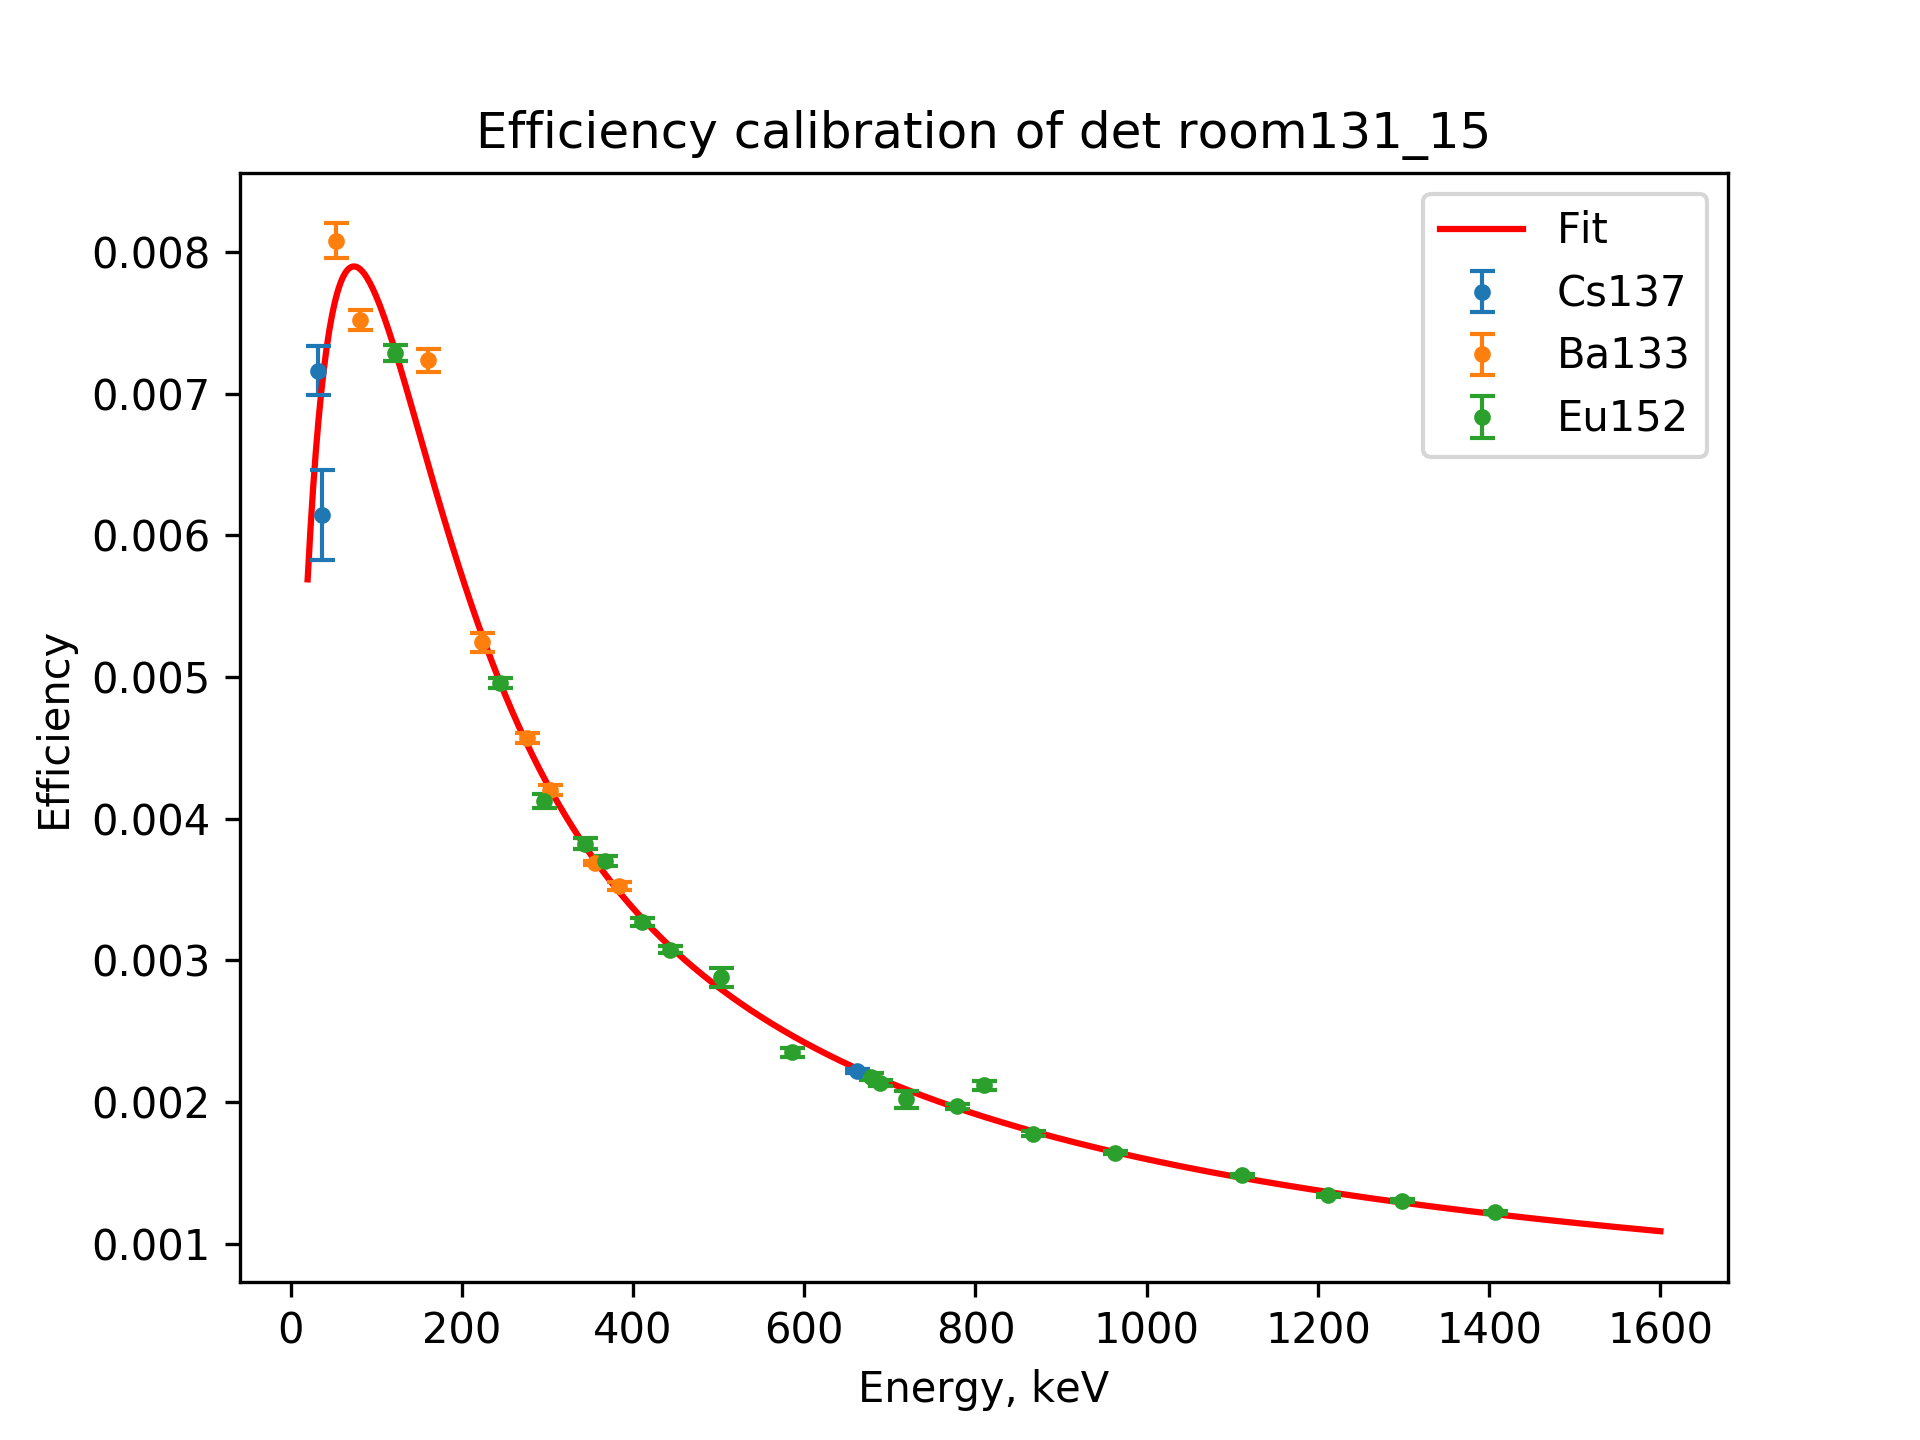
\includegraphics[width=0.6\textwidth]{Experiment/room131_15.png}
    \caption{An example of an efficiency curve with exact points calculated from equation \ref{eq:efficiency_analytical} and a curve fit from equation \ref{eq:efficiency_estimated}. }
    \label{fig:efficiency_curve}
\end{figure}

\section{End of beam activities}

The end of beam activities were estimated by extrapolating backwards in time, with the measured activities at various timepoints after the end of beam. The activities as a function of time sine EOB was calculated using equation \ref{eq:Final_Expression_A}, along with a self-attenuation correction: 

\begin{equation}
    A(\Delta t_d) = \frac{N_C\lambda}{\epsilon\I_\gamma (1-e^{-\lambda \Delta t_d})e^{-\mu\rho\Delta r/2}}
\end{equation}

where $\mu$ is the photoon attenuation coefficients from the XCOM photon cross section database+\footnote{https://www.nist.gov/pml/xcom-photon-cross-sections-database}, and $\rho\Delta r$ is the mass density of the foil. The gammas which were used are listed in tables \ref{tab:Products_Fe}, \ref{tab:Products_Ni}, \ref{tab:Products_Cu} and \ref{tab:Products_Ir} for iron, nickel, copper and iridium respectively. The gamma-ray self-attenuation (which is typically less than 0.2 \% (Iron paper, Andrew)) correction is based on the assumption that all activity that is made is located midway in the foil thicknesses. In reality however, the activity profile will follow the same shape as the excitation function over the energy range that expands over the foil, \textcolor{red}{if we assume that the stopping power dE/dx=0 which is a good estimation for thin foils less than 100 mg/cm$^2$??} (since activity and cross section are proportional). We do not know the excitation function ahead of time, and the excitation function does not change much either, since the foil thicknesses are so thin. So instead, this simplification is done, assuming that the average attenuation is through half of the foil thickness. \\ 

\noindent 
The equation describing the shape of the decay curve is given in equation \ref{eq:activity_decaylaw} for single decay or \ref{eq:ndecay_chains} for multiple decay. Decay chains of single and two-step decay (n=1,2) was sufficient in this analysis; 
\begin{equation} \label{eq:onestep_activity}
    A = A_0 e^{-\lambda \Delta t_d},\quad \text{ single step decay}
\end{equation}

and

\begin{equation} \label{eq:twostep_activity}
    A_2(t) = \lambda_n \Big[ A_{1,0}\lambda_1 \frac{(e^{-\lambda_1 } + e^{-\lambda_2})}{\lambda_1 - \lambda _2} + A_{2,0}e^{-\lambda_2 t} \Big],\quad \text{two step decay}
\end{equation}

where subnumber 1 is the parent nucleus, and subnumber 2 is the daughter nucleus. Parent activity is calculated from single step decay. The uncertainty was treated as \textcolor{red}{covarianced variables?} \\

The way in which the extrapolation was done was the scipy optimize curve fit function, where the $A_0$ of the daughter was the optimizing parameter. Since there is only one optimized parameter, there was no covariance and the uncertainty was calculated using equation \ref{eq:uncertainty_simplification}.  In the cases where neither parent or daughter activity were known, which were the case for the monitor reaction $^{58}Co$ with $^{58m}$Co decaying into the ground state by internal conversion, both parent and daughter activity were optimizing parameters which are very correlated and thus the uncertainty in end of beam activity was calculated \ref{eq:variance_full}. Figure \ref{fig:activity_curves} shows two examples of the two different activity curves; one step decay for $^{193m}$Pt ($t_{1/2}$=4.33 days) and two step decay for the monitor product $^{58}$Co ($t_{1/2}$=70.86 days) with feeding from the isomer $^{58m}$Co ($t_{1/2}$=9.10 hours).  


\begin{figure}%
    \centering
    \subfloat[Activity of $^{193m}$Pt ($t_{1/2}$=4.33 d) produced from iridium. The end of beam activity was estimated using a one step decay (equation \ref{eq:onestep_activity})]{{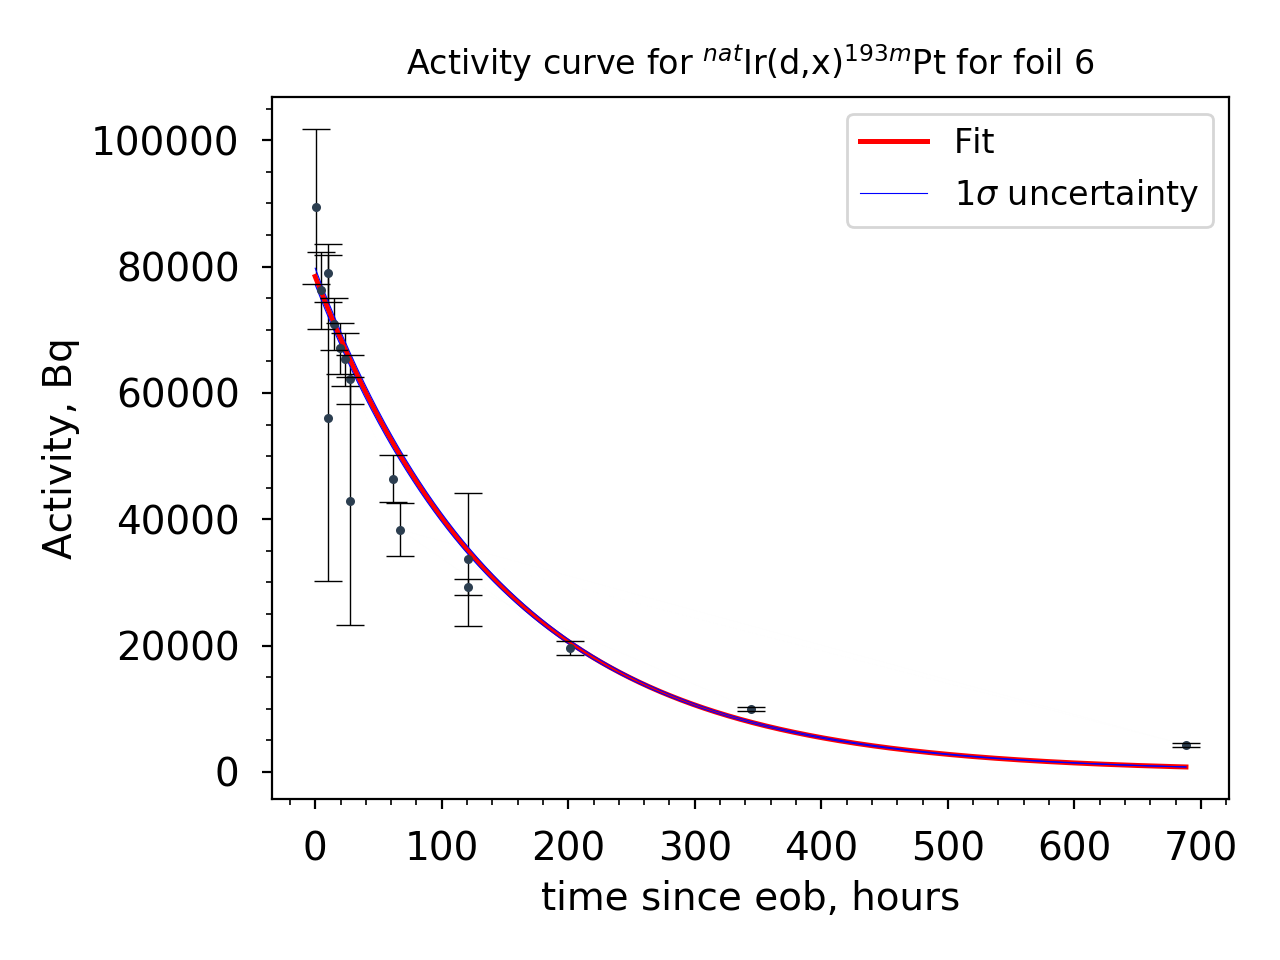
\includegraphics[width=11cm]{Analysis/activity_Ir_193mPt_f6.png} }}\hfill
    \subfloat[Activity of $^{58}$Co ($t_{1/2}$=70.86 d) produced from nickel. The end of beam activity is estimated using a two step decay (equation \ref{eq:twostep_activity}. The feeding is from $^{58m}$Co ($t_{1/2}$=9.10 h.) ]{{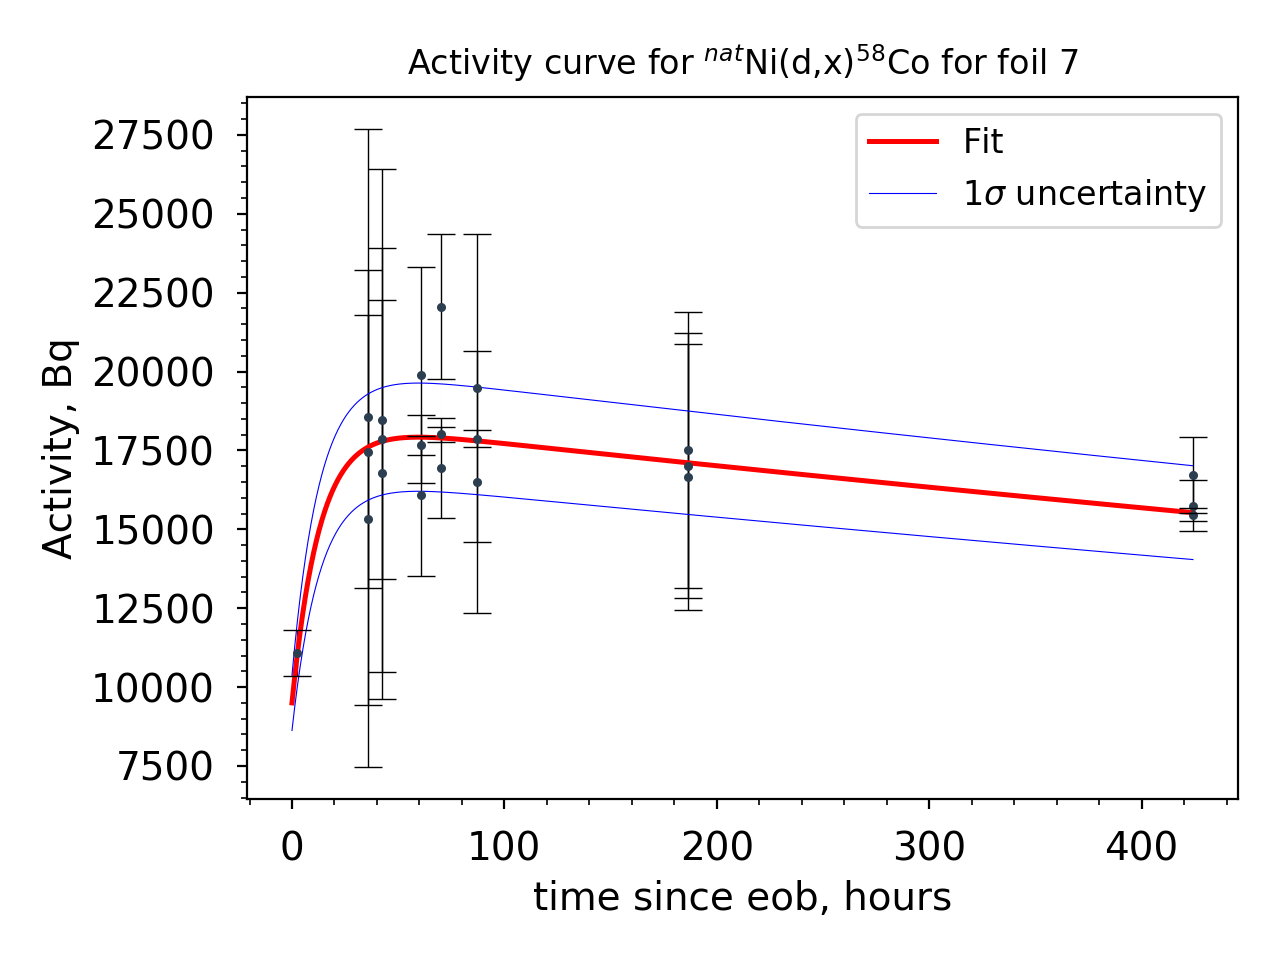
\includegraphics[width=11cm]{Analysis/activity_Ni_56Co_f7.png} }}%
    \caption{Two examples of activity curves. The uncertainty in activity decreases with increasing time since end of beam which is due to longer counts decreases the uncertainty. (from theory, counting statistics)  }%
    \label{fig:activity_curves}%
    
\end{figure}

\end{comment}
\begin{comment}
\section{Estimation of the beam current and beam energy assignments}
The beamintegrator measured a current of 128.5 nA in front of the beam stack. However in order to have precise cross section measurements, the nominal beam current in each foil was calculated. The IAEA recommended monitor reactions (2017) $^\text{nat}$Ni(d,x)$^{61}$Cu,$56,58$Co, $^\text{nat}$Cu(d,x)$^{62,63,65}$Zn and $^\text{nat}$Fe(d,x)$^{56}$Co \cite{Hermanne2018a} were used to obtain a weighted average beam current in each foil solving equation \ref{eq:Final_Expression_A0} for beam current $\Phi$:

\begin{equation} \label{eq:BC_simple}
    \Phi(E) = \frac{A_0}{N_T \sigma(E)_\text{mon}(1-e^{-\lambda \Delta t_\text{irr}})}
\end{equation}
\noindent 
where $A_0$ is the end of beam activities for the monitor products from the spectra, $N_T$ is the number of target nuclei calculated from the mass density $\rho\Delta r$, $\sigma_\text{mon}$ is the monitor cross sections. Equation \ref{eq:BC_simple} builds upon the thin target assumption, which implies that the energy degradation in the foil is zero. However, we know that there is an energy distribution in each foil. This energydistribution was modeled using the Monte-Carlo based npat ziegler code  

which was estimated using NPAT's (Nuclear Physics Analysis Tool) Ziegler simulation\footnote{John's code, must cite.}. The ziegler code simulates the deuteron transport based upon the Anderson \& Ziegler stoppingpower formalism. Bethe-Block 

Anderson \& Ziegler is an empirical stopping power formalism, does not have any physics derivation behind it, and is a tuned model which reproduces experimental data. Bethe-Block is derived from basic E\&M with no tuned parameters. Bethe-Block also gives the purely electronic stopping power, the stopping power from an ion's interaction with the electronic cloud of an atom in the stopping medium. However the total stopping power is the sum of electronic, nuclear (elastic and inelastic scattering) and radiative stopping power, which is what we actually want frmo the experimental standpoint. Bethe-Block ignores nuclear and radiative. 



, using Monte Carlo simulations \textcolor{red}{write a few sentences in theory..}. The code provides the full deuteron energy and flux degradation in each foil, $d\phi/dE$, which can be visualized for the iridium foils in figure \ref{fig:ir_energyflux}.  Can be seen that as the deuteron energy is degraded, the mean value is shifted towards the low energy side, and the the peak width increases. As stoppingpower is inversely proportional to the charge particle energy ($-\frac{dE}{dx}\propto \frac{1}{\beta^2}$, bethe block), and along with scattering taking place towards the end of stack, the low energy tail is more degraded, and we see a skew towards the low energy, creating a broader energy-flux profile and a shift of the mean value (centroid). This shift leads to an increasing uncertainty in energy. The (normalized) flux-weighted average energy for each foil was calculated, \textcolor{blue}{ironpaper: which takes into account the slowing down of of deuterons, and reports effective energy centroid of each foil}, using the energy distributions $d\phi/dE$ provided by the Ziegler code:

\begin{equation} \label{eq:flux_weighted_average_energy}
    \langle E \rangle = \frac{\int E \frac{d\phi}{dE}dE}{\int \frac{d\phi}{dE}dE}
\end{equation}

The uncertainty in beam energy is divided into low energy and high energy tale, with the FWHM split by the centroid (figure \ref{fig:ir_energyflux}). 

Likewise, the energydependent monitor IAEA cross sections need to be flux-weighted over each foil. In order to do this, a spline interpolation over the energy array over each foil provided by the Ziegler simulation was spline interpolated with the IAEA recommended cross section data. Thus, the monitor cross section in equation \ref{eq:BC_simple} is modified to 

\begin{equation}
    \sigma (\langle E\rangle) = \frac{\int \sigma_\text{mon} \frac{d\phi}{dE}dE}{\int \frac{d\phi}{dE}dE}
\end{equation}


\begin{figure}
    \centering
    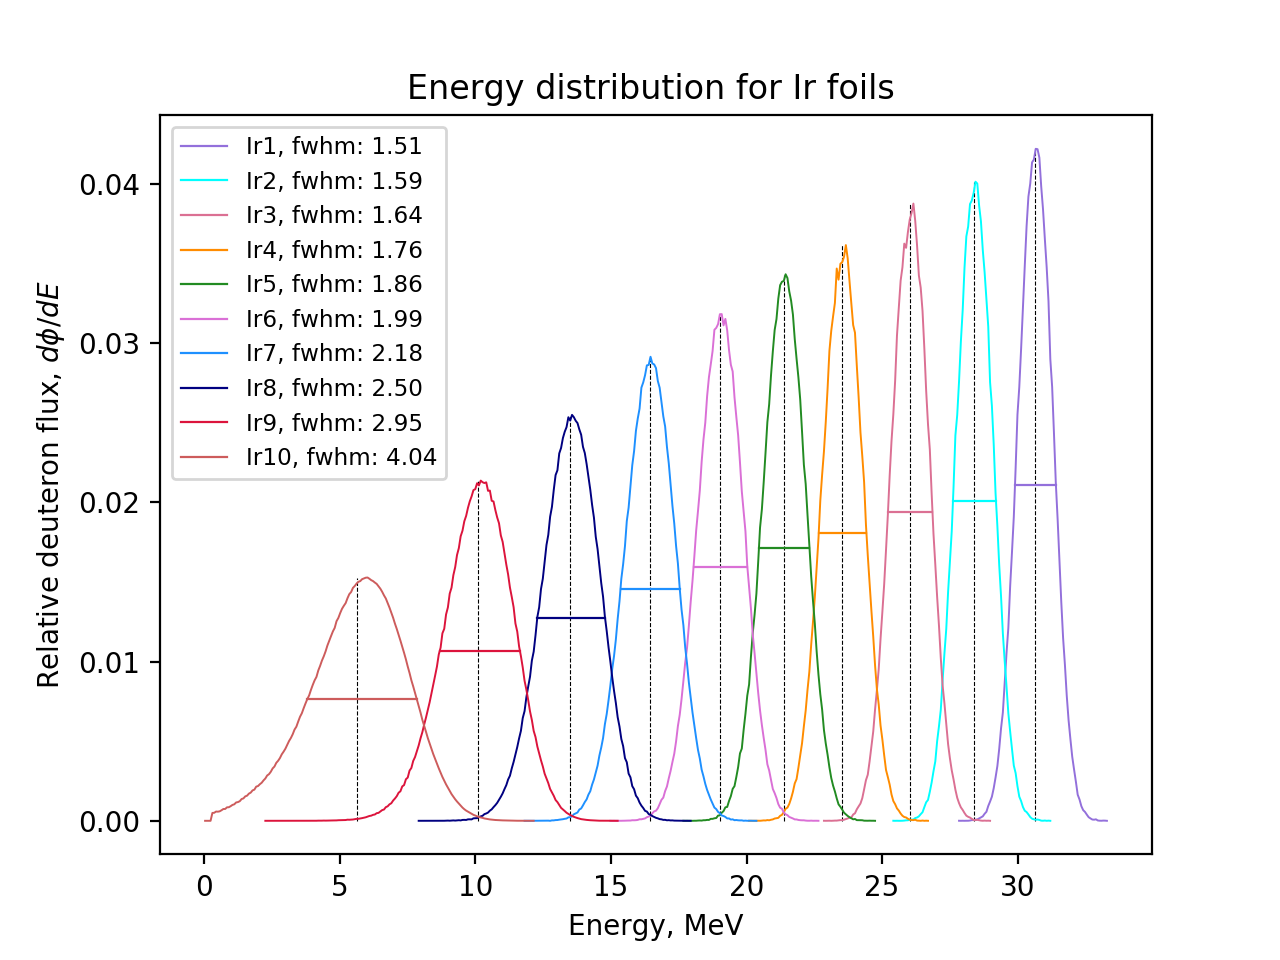
\includegraphics{Analysis/Ir_flux_distribution_B_+2_D_+4,25.png}
    \caption{Iridium energy flux distribution over the 10 foils. As the energy degrades, scewed and larger full width half max. The vertical line in each peak is the mean value. This indicates that at lower energies, the right uncertainty is greater than the left uncertainty in the peak.}
    \label{fig:ir_energyflux}
\end{figure}

With the end of beam activities for the monitor reactions, number of target nuclei and the flux- weighted IAEA cross sections, the beam current as a function of the flux-weighted average beam energy was estimated for each reaction in each foil. 

\subsection{Variance minimization of the deuteron transport calculations}
In theory, the estimated beam current of a charge particle beam should be constant, until completely stopped, since the majority of the incident particles does not interact in nuclear reactions, but only lose energy via elastic and inelastic scattering. However, non-consistant values of the beam current, especially in the back of the stack can be due to energy bins being assigned wrongly in the energy distribution simulation done in Ziegler or a systematic error in the areal density which gets progressively worse further back in the stack (Niobium paper, Andrew). A way to work around these errors was to perform a variance minimization varying the beam energy and the areal density of the foils with 20\% increase and decrease systematically, and estimate the reduced $\chi^2$ (equation \ref{eq:chisq_DOF}) over compartment 3,6 and 9. Variance minimization (Andrew's Niobium and iron paper + \foonote{https://sci-hub.tw/https://doi.org/10.1016/j.nimb.2016.09.018}). \\

 For compartment 3 ($E_d$=25 MeV) all seven monitor reactions were above threshold,  thus 6 degrees of freedom.  However,  early in the target stack,  the scattering was low, and the $\chi^2$ does not tell how well the energy bin assignment work further back in the stack.  For compartment 6 ($E_d$=18 MeV), all the six possible monitor reactions (for nickel and copper) were above threshold, and it gave a good estimate of how the beam current was developing throughout the stack.  In compartment 9 ($E_d$=10 MeV), five monitor reactions are above threshold (except for $^{62}$Zn).  At the very end it is possible to see the full effect of the scattering.\\

With the assumption that the beamcurrent loss is zero over one compartment, a linear fit-model (using the scipy optimize curvefit function) with a slope equal to zero was used to estimate the beam current in each compartment, and with the estimated $\chiˆ2$.  

Figure \ref{fig:BC_comp6} shows the uncertainty weighted linear fit over compartment 6. 

\begin{figure}
    \centering
    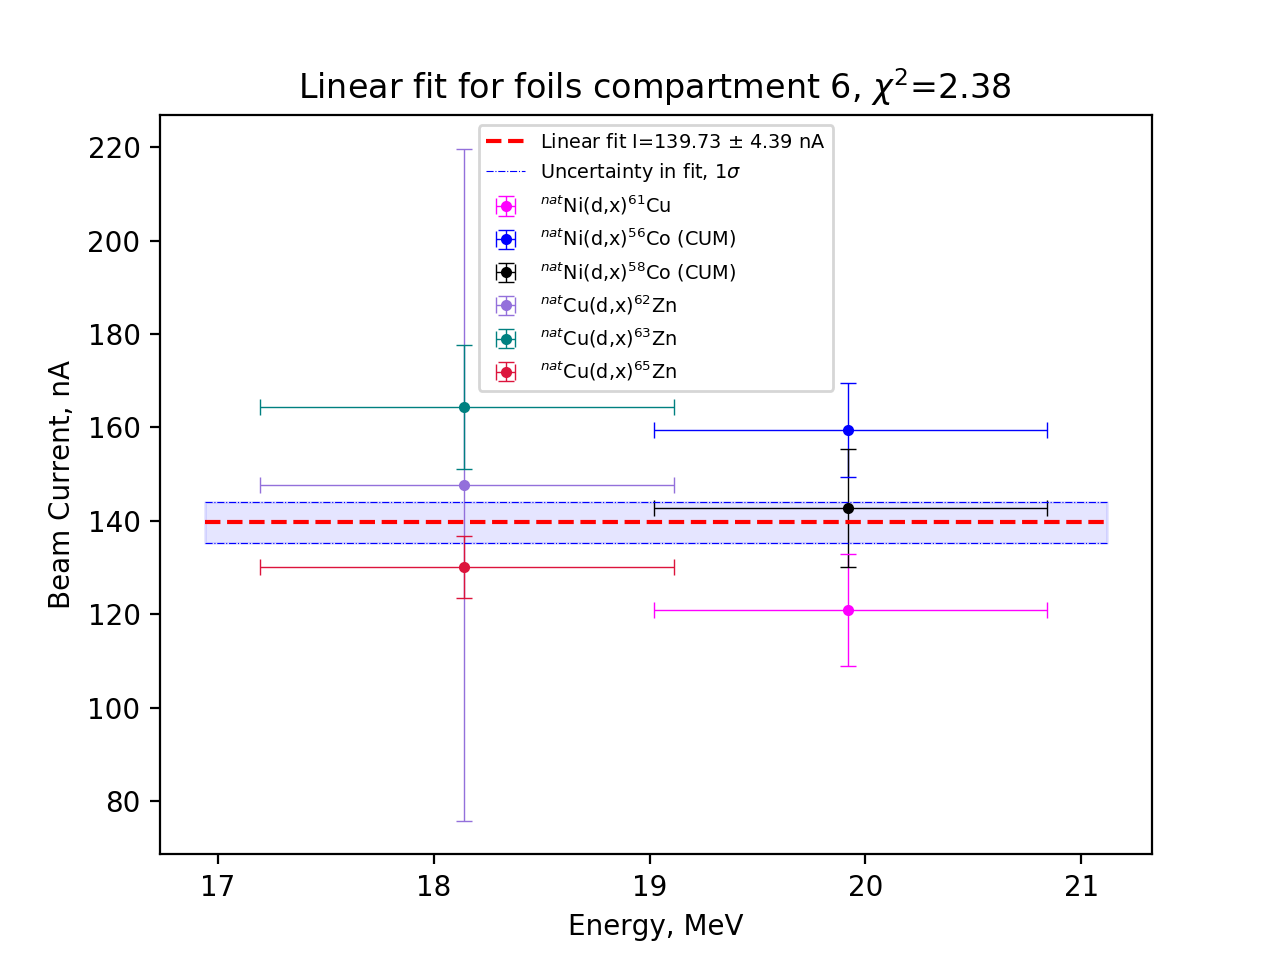
\includegraphics{Analysis/Compartment_6.png}
    \caption{The estimated (uncertainty weighted) beamcurrent over compartment 6. }
    \label{fig:BC_comp6}
\end{figure}

Figure \ref{fig:varmin_beamcurrent} shows the beam current before and after variance minimization, and the weighted average beam currents are listed in table \ref{tab:weighted_BC} estimated before and after the variance minimization. After variance minimization, the beam current estimated in each compartment (stabled lines) were similar, and meanwhile the weighted $\chi^2$ was about the same in compartment 6, it has improved in compartment 3 and very visible in compartment 9. In general the points are also more aligned. 

\begin{figure}%
    \centering
    \subfloat[]{{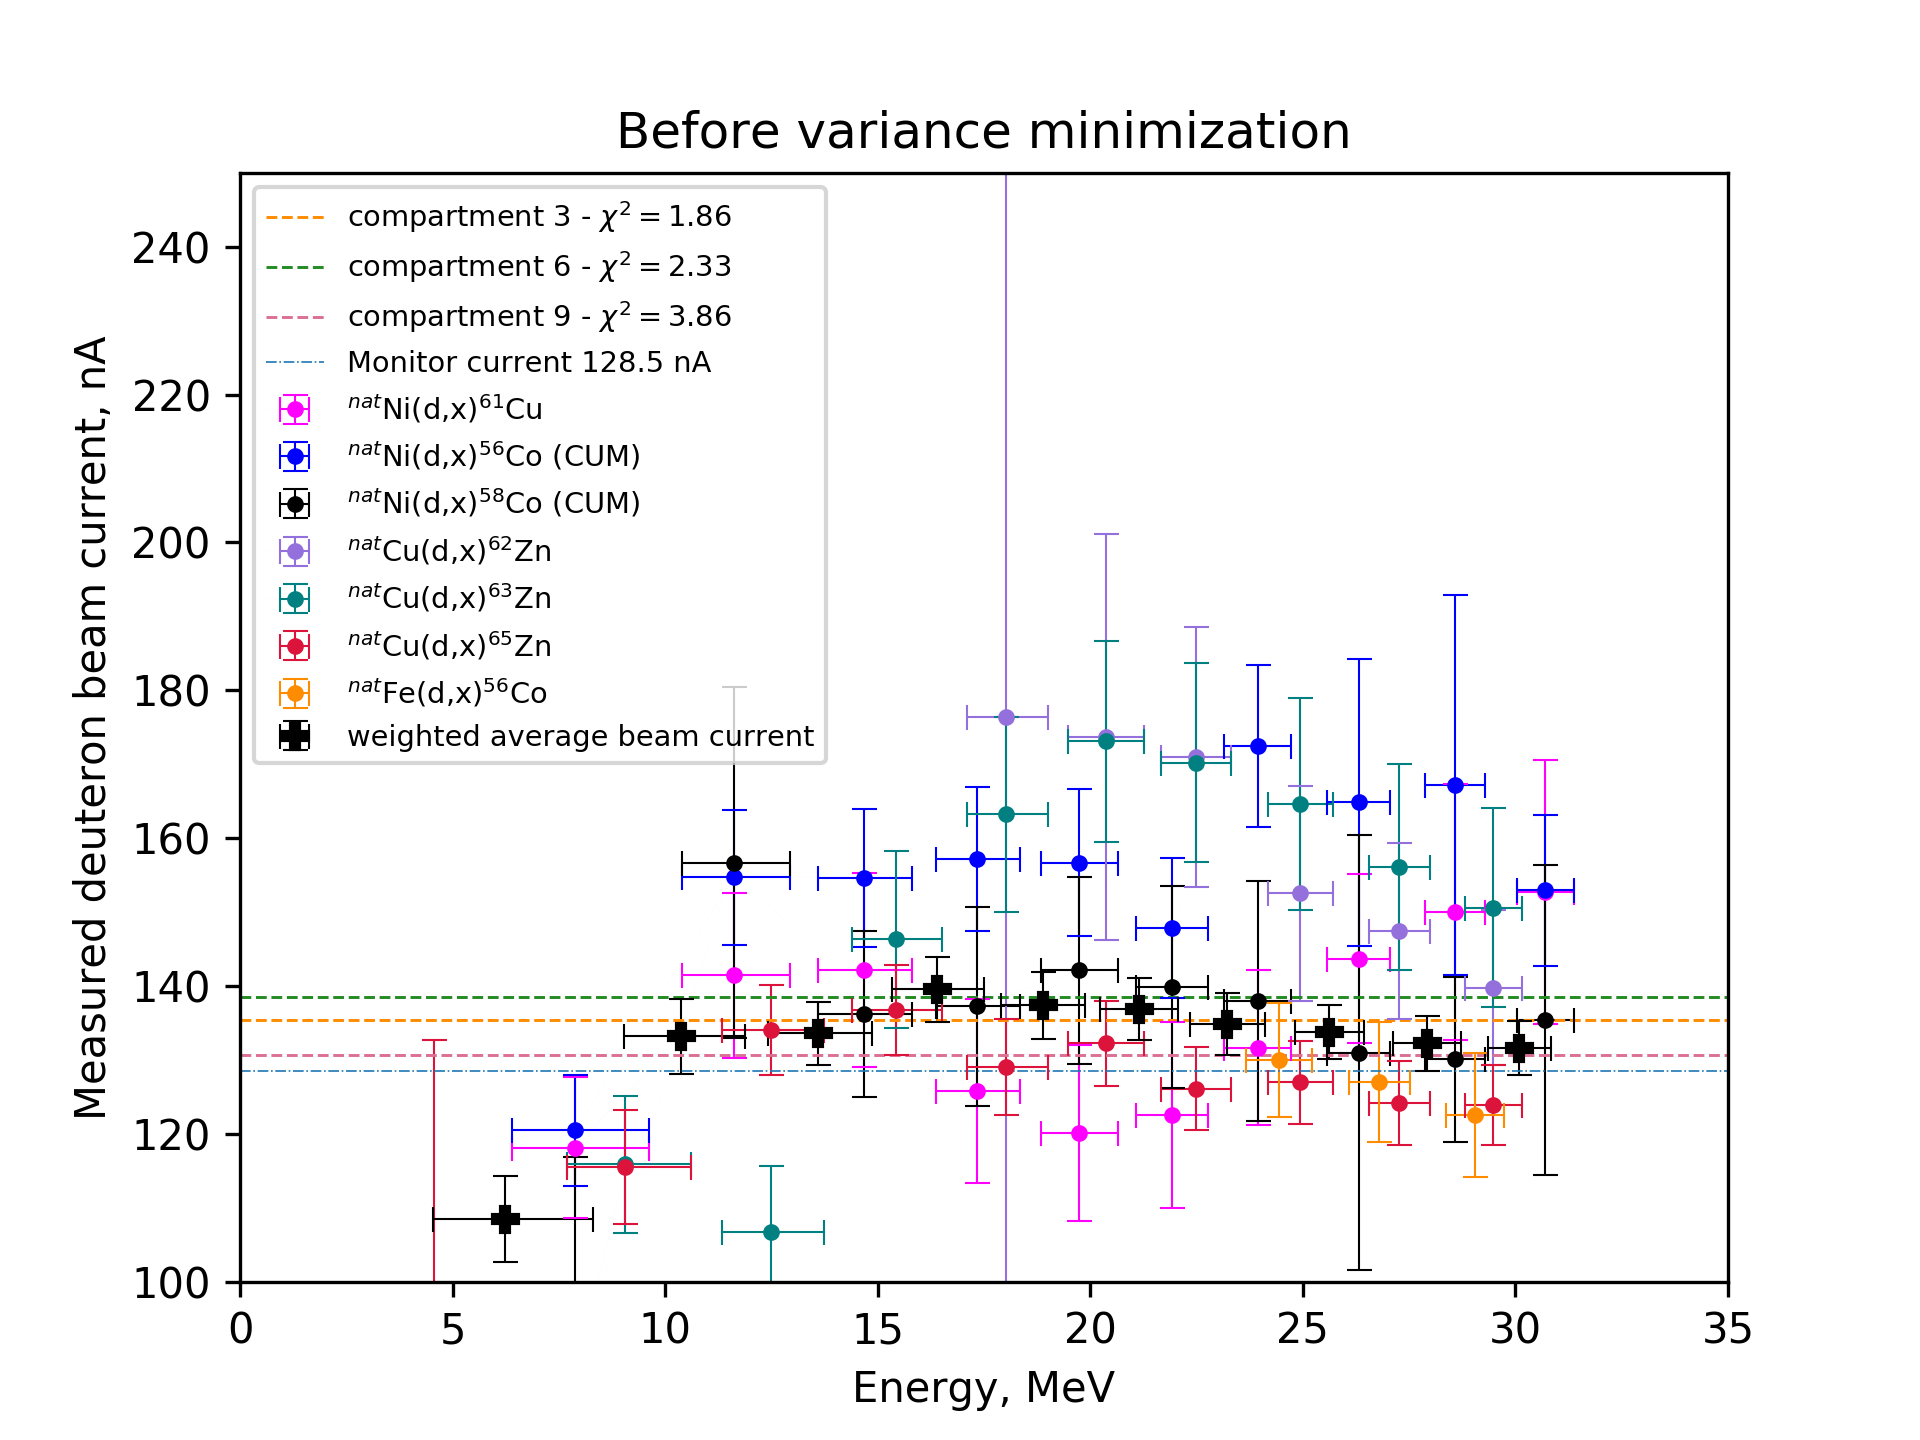
\includegraphics[width=11cm]{Analysis/beamcurrent_B_0_D_0.png} }}\hfill
    \subfloat[A 2\% increase in beam current and a 4.25\% increase in areal density gave the overall most consistent beam current, with reasonable values for the weighted . ]{{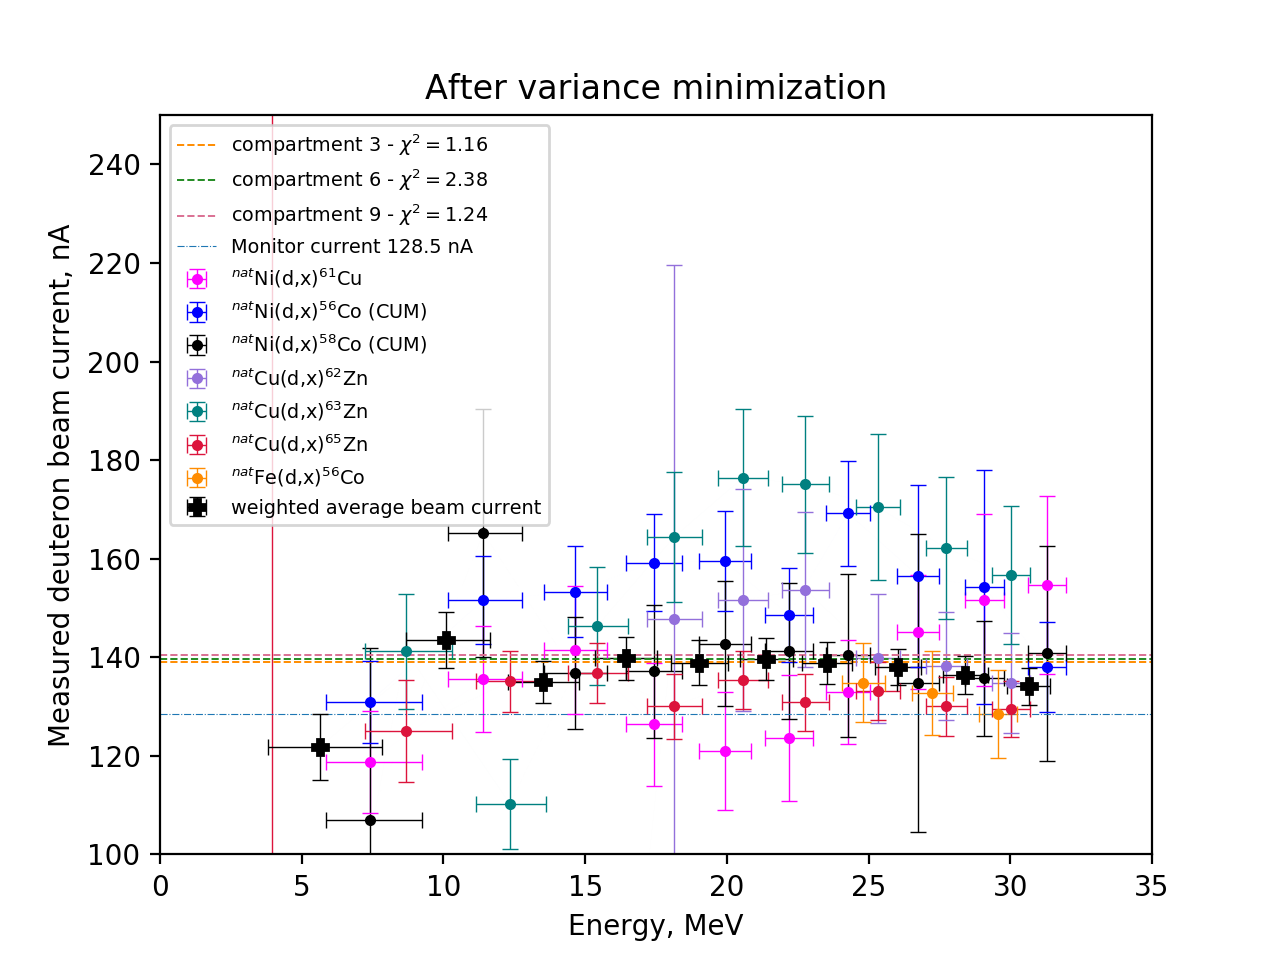
\includegraphics[width=11cm]{Analysis/beamcurrent_B_+2_D_+4,25.png} }}%
    \caption{Beam current before and after variance minimization.  }%
    \label{fig:varmin_beamcurrent}%
\end{figure}

\begin{table}[]
    \centering
        \caption{The weighted average beam current before and after variance minimization in each compartment. The beam current on the 88-Inch Cyclotron beam integrator was 128.5 nA.}
    %\footnotesize
    \begin{tabular}{c |c c}
        \hline 
       Compartment & \makecell{Before} & \makecell{After}\\ 
        \hline 
        \makecell{01} & \makecell{131.56 \pm 3.64} & \makecell{134.08 \pm 3.70}  \\ 
        \makecell{02} & \makecell{132.23 \pm 3.74} & \makecell{136.42 \pm 3.83} \\ 
        \makecell{03} & \makecell{133.81 \pm 3.64 } & \makecell{138.02 \pm 3.75} \\ 
        \makecell{04} & \makecell{134.89 \pm 4.21 } &  \makecell{138.88 \pm 4.31}\\ 
        \makecell{05} &\makecell{136.85 \pm 4.21} & \makecell{139.67 \pm 4.29} \\
        \makecell{06} &\makecell{137.40 \pm 4.53} & \makecell{138.85 \pm 4.58} \\
        \makecell{07} &\makecell{139.55 \pm 4.37} & \makecell{139.77 \pm 4.37} \\
        \makecell{08} &\makecell{133.60 \pm 4.27} & \makecell{134.96 \pm 4.32}\\
        \makecell{09} &\makecell{133.16 \pm 5.04} & \makecell{143.59 \pm 5.67} \\
        \makecell{10} &\makecell{108.49 \pm 5.80} & \makecell{121.75 \pm 6.65} \\
    
         %\makecell{Before} & \makecell{131.56 \pm 3.64} & \makecell{132.23 \pm 3.74} & \makecell{133.81\pm3.64 } & \makecell{134.89\pm 4.21 } & \makecell{136.85_{\pm 4.21}} & \makecell{137.40 \pm 4.53} & \makecell{139.55 \pm 4.37} & \makecell{133.60 \pm 4.27} & \makecell{133.16 \pm 5.04} & \makecell{108.49 \pm 5.80}  \\
         %\makecell{After} & \\
    \end{tabular}
    \label{tab:weighted_BC}
\end{table}
\end{comment}
\begin{comment}
\section{Energy and Beam current}



For the equation for cross section (equation \ref{eq:cross_section_equation}), the beam current $\Phi(E)$ must be known. The beam integrator measured 128.5 nA, which is the current entering the stack. However, due to large energy degradation in the energy stack, there will be a certain spread of the beam, following scattering. In addition, there have not been an experiment with deuterium on a target stack before, so we also needed to see how much deuteron break up affected the current throughout the stack. Monitor reactions are reactions with well-known cross sections\footnote{https://www-nds.iaea.org/medical/monitor_reaction_article.pdf}. The IAEA recommended cross sections for $^\text{nat}$Fe(d,x)$^{56}$Co, $^\text{nat}$Ni(d,x)$^{61}$Cu, $^\text{nat}$Ni(d,x)$^{56,58}$Co and $^\text{nat}$Cu(d,x)$^{62,63,65}$Zn (\textcolor{red}{write about Q value, half life}) were used to estimate a more sensitive deuteron beam current throughout the stack. By solving \ref{eq:cross_section_equation} for beam current, the beamcurrent throughout the stack can be estimated

\begin{equation}
    \Phi(E) = \frac{A_0}{N_T (1-e^{-\lambda \Delta t_\text{irr}})\sigma(E)_\text{mon}}
\end{equation}

In cross section experiments using thin targets\footnote{Special curriculum p. 14}, the suggested value is a flux average cross section, which implies that the cross section is dependent on the flux-weighted average beam energy. One single foil thus provides one cross section measurement, with the uncertainty in energy only being dependent on the energy distribution in each foil. For thin targets, a stopping power $dE/dx=0$ is assumed which is a very good approximation for targets which are less than 50 mg/cm$^2$ \textcolor{red}{cite?}.   

Normalized differential beam current  (\textcolor{red}{need some help understanding this in detail})
\begin{equation}
    \sigma(E)_\text{mon}=\frac{\int \sigma(E)\frac{d\phi}{dE}dE}{\int \frac{d\phi}{dE}dE}
\end{equation}

\textcolor{blue}{From niobium paper: Since stoppingpower is inversely proportional for to cp energy, the low energy tail of the energy distribution is degraded more in each stack element than the high energy tail. This effect compounds to towards the rear of the stack, creating a significantly broadened low energy tail, and a progressevely larger net shift of the centroid to a lower energy. To account for this increasing energy uncertainty, a suitably representative energy must be established for each foil of the target stack. The flux weighted average deuteron energy in each foil $\langle E \rangle$ represents the energy centroid for deuterions in a target stack using the energy distributions from $d\phi/dE$ from the Ziegler stopping power deuterion transport }
\begin{equation}
    \langle E \rangle = \frac{\int E \frac{d\phi}{dE}dE}{\int \frac{d\phi}{dE}dE}
\end{equation}

where $\sigma(E)$ is the IAEA recommended cross section, $\frac{d\phi}{dE}$ is the energy dependent deuteron flux through each foil. The deuteron flux (or energy degradation) was estimated using a code called NPAT's (nuclear physics analysis tool) Ziegler simulation\footnote{https://pypi.org/project/npat/}. NPAT uses the Anderson \& Ziegler formalism for calculating charged-particle stopping powers in matter in a stack with targets. \textcolor{red}{write a few sentences about this in the theory!}. The code thus simulates the deuteron flux as a function of energy in the beam stack (assigned to a foil).

Figure \ref{fig:ir_energyflux} shows an overview of the flux-energy distribution in each foil for Iridium. The other monitor foils have the same functions.  \textcolor{red}{Write about recommended data, the spline function etc etc.. }

\begin{figure}
    \centering
    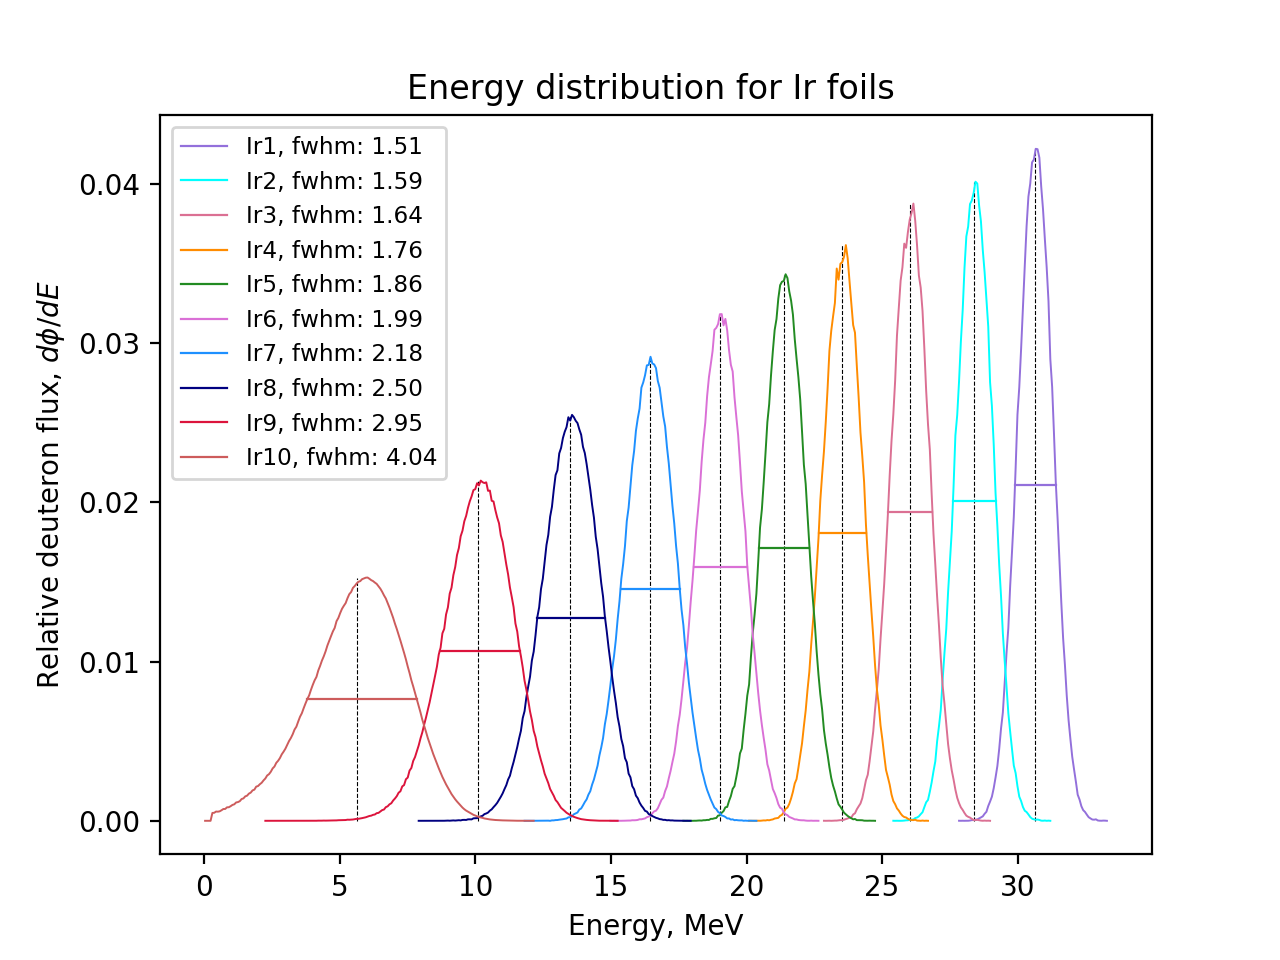
\includegraphics{Analysis/Ir_flux_distribution_B_+2_D_+4,25.png}
    \caption{Iridium energy flux distribution over the 10 foils. As the energy degrades, scewed and larger full width half max. The vertical line in each peak is the mean value. This indicates that at lower energies, the right uncertainty is greater than the left uncertainty in the peak.}
    \label{fig:ir_energyflux}
\end{figure}

\textcolor{red}{need some info from andrew here}

\subsection{Variance minimization}
\textcolor{blue}{From Niobium paper p. 57: In theory, the beam current should be more or less constant through the stack, even though the deuterons lose energy. Variance minimization is a technique to reduce the uncertainty in the deuteron beam energies. Non-consistent values  for the beam current further back in the stack can be wrong energy bin assignments in the modeled energy distribution (ziegler), or a systematic error in the areal density, which gets progressively worse further back in the stack, "due to the compound effect of systematic uncertainties in stack areal densities"}. The areal density and the beam energy was varied with 20\% increase and decrease, and the reduced $\chi^2$ (equation \ref{eq:chisq_DOF}) was estimated over compartment 3, 6 and 9. For compartment 3 ($E_d\simeq$25 MeV) all seven monitor reactions were above threshold, thus 6 degrees of freedom. However, early in the target stack, the scattering was low, and the $\chi^2$ does not tell how well the energy bin assignment work further back in the stack. For compartment 6 ($E_d\simeq$18 MeV), all the six possible monitor reactions (from nickel and copper) were above threshold, and it gave a good estimate of how the beam current was developing throughout the stack. In compartment 9 ($E_d\simeq$10 MeV), five monitor reactions are above threshold (except for $^{62}$Zn). At the very end it is possible to see the full effect of the scattering. \\

\noindent 
The beamcurrent loss is assumed zero in one compartment, so a linear beam current fit would have a slope equal to zero. The estimated beam current in each compartment was estimated using the scipy curve fit function, with a straight line as model. Figure \ref{fig:BC_comp6} shows the uncertainty weighted linear fit over compartment 6. 

\begin{figure}
    \centering
    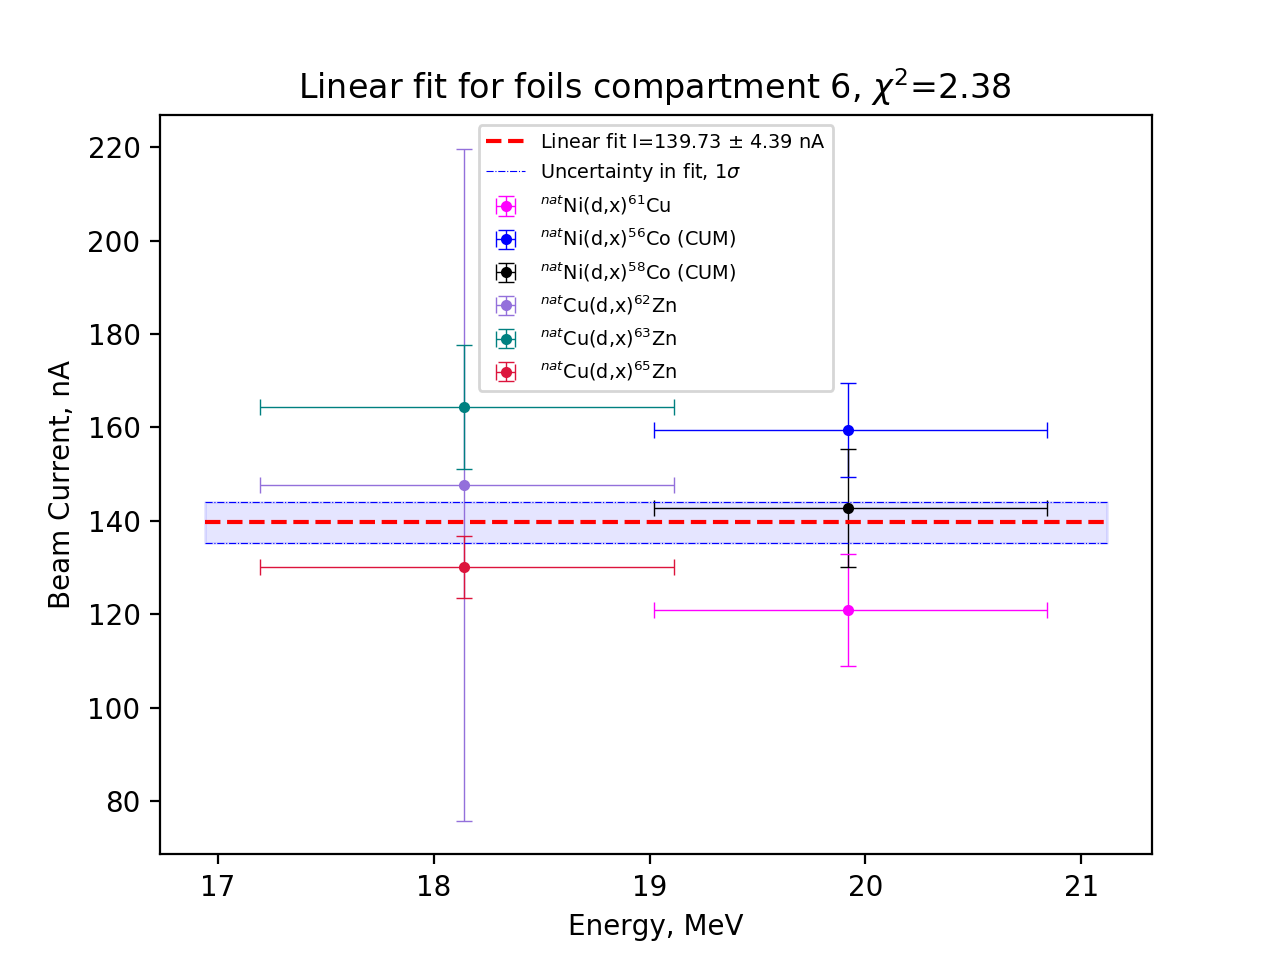
\includegraphics{Analysis/Compartment_6.png}
    \caption{The estimated (uncertainty weighted) beamcurrent over compartment 6. }
    \label{fig:BC_comp6}
\end{figure}

Figure \ref{fig:varmin_beamcurrent} shows the beam current before and after variance minimization, and the weighted average beam currents are listed in table \ref{tab:weighted_BC} estimated before and after the variance minimization. After variance minimization, the beam current estimated in each compartment (stabled lines) were similar, and meanwhile the weighted $\chi^2$ was about the same in compartment 6, it has improved in compartment 3 and very visible in compartment 9. In general the points are also more aligned. 

\begin{figure}%
    \centering
    \subfloat[]{{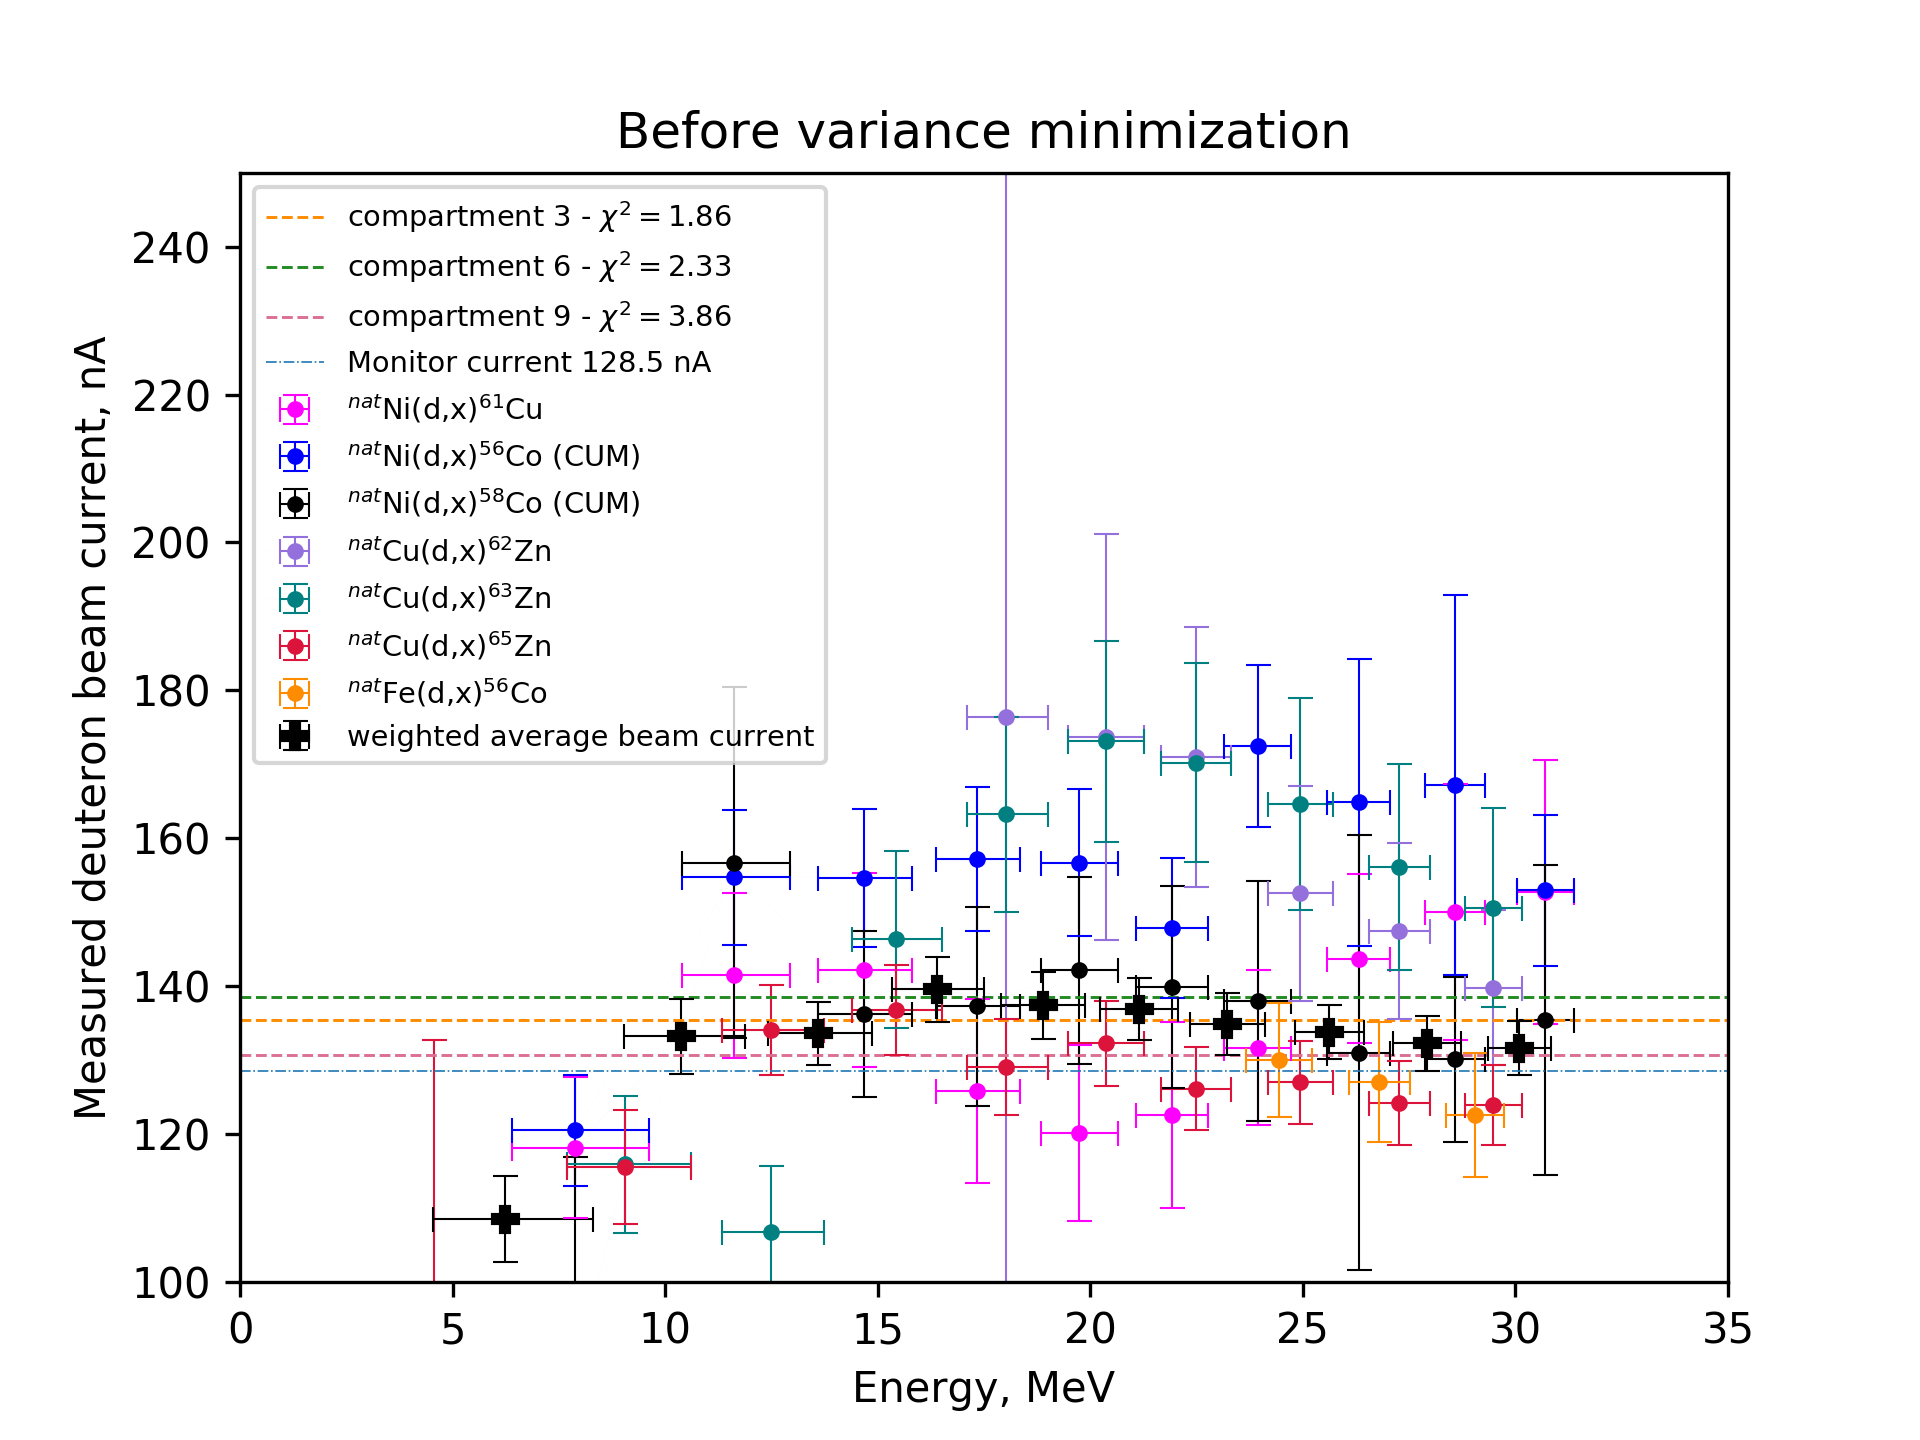
\includegraphics[width=11cm]{Analysis/beamcurrent_B_0_D_0.png} }}\hfill
    \subfloat[A 2\% increase in beam current and a 4.25\% increase in areal density gave the overall most consistent beam current, with reasonable values for the weighted . ]{{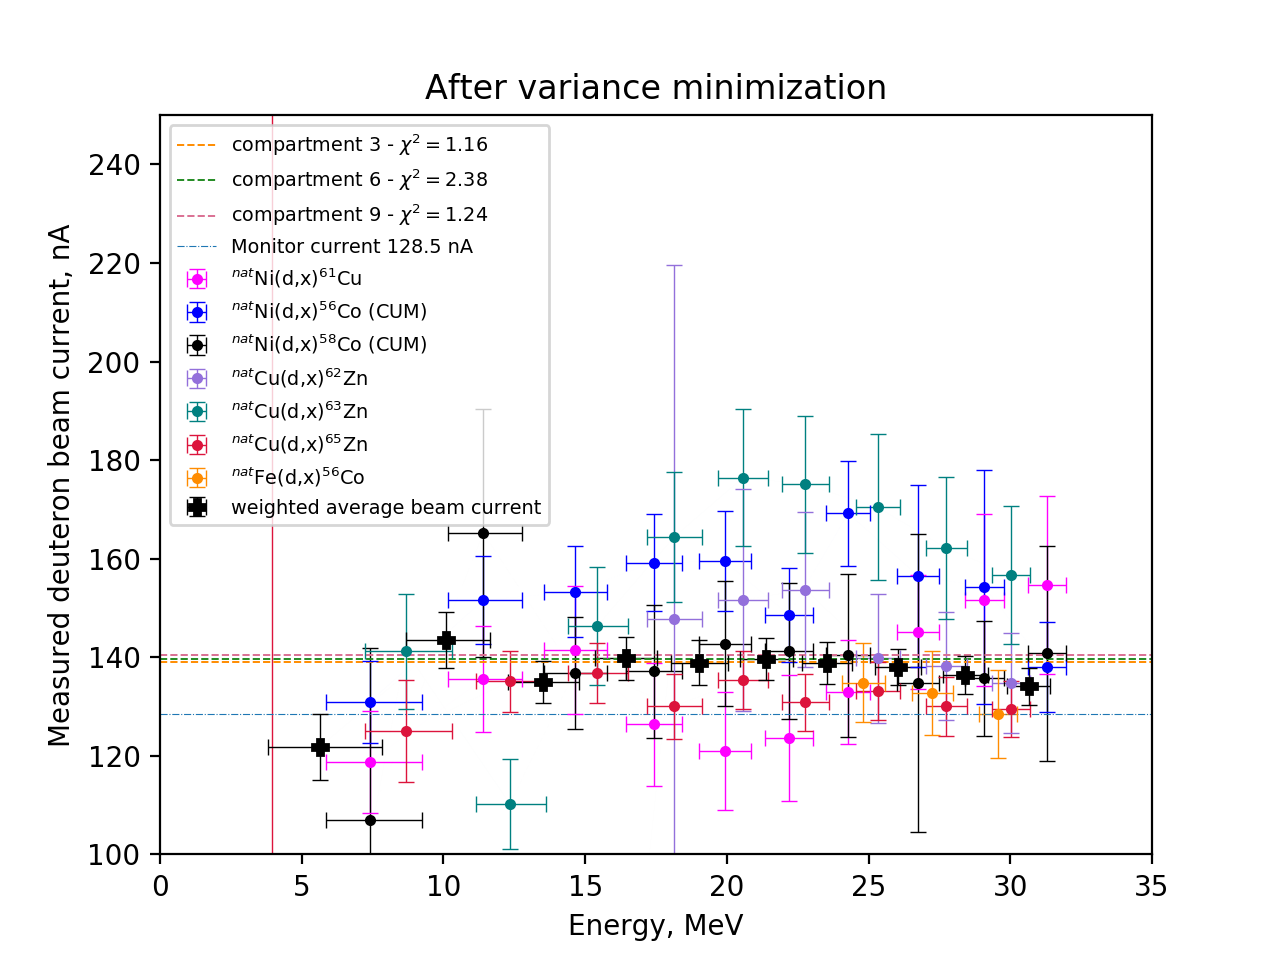
\includegraphics[width=11cm]{Analysis/beamcurrent_B_+2_D_+4,25.png} }}%
    \caption{Beam current before and after variance minimization.  }%
    \label{fig:varmin_beamcurrent}%
\end{figure}


\begin{table}[]
    \centering
        \caption{The weighted average beam current before and after variance minimization in each compartment. The beam current on the 88-Inch Cyclotron beam integrator was 128.5 nA. }
    %\footnotesize
    \begin{tabular}{c|c c c c c c c c c c}
        & \makecell{c_{10}} & \makecell{c_{09}} & \makecell{c_{08}} & \makecell{c_{07}} & \makecell{c_{06}} & \makecell{c_{05}} & \makecell{c_{04}} & \makecell{c_{03}} & \makecell{c_{02}} & \makecell{c_{01}} \\ 
        \hline
         \makecell{Before} & \makecell{131.56_{\pm 3.64}} & \makecell{132.23_{\pm 3.74}} & \makecell{133.81_{\pm3.64 }} & \makecell{134.89_{\pm 4.21 }} & \makecell{136.85_{\pm 4.21}} & \makecell{137.40 _{\pm 4.53}} & \makecell{139.55_{\pm 4.37}} & \makecell{133.60_{\pm 4.27}} & \makecell{133.16_{\pm 5.04}} & \makecell{108.49_{\pm 5.80}}  \\        
         %\makecell{Before} & \makecell{131.56 \pm 3.64} & \makecell{132.23 \pm 3.74} & \makecell{133.81\pm3.64 } & \makecell{134.89\pm 4.21 } & \makecell{136.85_{\pm 4.21}} & \makecell{137.40 \pm 4.53} & \makecell{139.55 \pm 4.37} & \makecell{133.60 \pm 4.27} & \makecell{133.16 \pm 5.04} & \makecell{108.49 \pm 5.80}  \\
         \makecell{After} & \\
    \end{tabular}
    \label{tab:my_label}
\end{table}


\begin{table}[]
    \centering
        \caption{The weighted average beam current before and after variance minimization in each compartment. The beam current on the 88-Inch Cyclotron beam integrator was 128.5 nA.}
    %\footnotesize
    \begin{tabular}{c |c c}
        \hline 
       Compartment & \makecell{Before} & \makecell{After}\\ 
        \hline 
        \makecell{01} & \makecell{131.56 \pm 3.64} & \makecell{134.08 \pm 3.70}  \\ 
        \makecell{02} & \makecell{132.23 \pm 3.74} & \makecell{136.42 \pm 3.83} \\ 
        \makecell{03} & \makecell{133.81 \pm 3.64 } & \makecell{138.02 \pm 3.75} \\ 
        \makecell{04} & \makecell{134.89 \pm 4.21 } &  \makecell{138.88 \pm 4.31}\\ 
        \makecell{05} &\makecell{136.85 \pm 4.21} & \makecell{139.67 \pm 4.29} \\
        \makecell{06} &\makecell{137.40 \pm 4.53} & \makecell{138.85 \pm 4.58} \\
        \makecell{07} &\makecell{139.55 \pm 4.37} & \makecell{139.77 \pm 4.37} \\
        \makecell{08} &\makecell{133.60 \pm 4.27} & \makecell{134.96 \pm 4.32}\\
        \makecell{09} &\makecell{133.16 \pm 5.04} & \makecell{143.59 \pm 5.67} \\
        \makecell{10} &\makecell{108.49 \pm 5.80} & \makecell{121.75 \pm 6.65} \\
    
         %\makecell{Before} & \makecell{131.56 \pm 3.64} & \makecell{132.23 \pm 3.74} & \makecell{133.81\pm3.64 } & \makecell{134.89\pm 4.21 } & \makecell{136.85_{\pm 4.21}} & \makecell{137.40 \pm 4.53} & \makecell{139.55 \pm 4.37} & \makecell{133.60 \pm 4.27} & \makecell{133.16 \pm 5.04} & \makecell{108.49 \pm 5.80}  \\
         %\makecell{After} & \\
    \end{tabular}
    \label{tab:weighted_BC}
\end{table}
\end{comment}
\begin{comment}
For cross section calculations, equation \ref{eq:CrossSection_general} is used, with the estimated weighted average beam current. Figure \ref{fig:monitor_BC+CS} shows the estimated cross sections for the monitor reactions, using the weighted average beam current over all monitor foils. The recommended monitor cross section data for the monitor reactions are also plotted, which was used in the cross section calculation.  



\begin{figure}%
    \centering
    \subfloat[]{{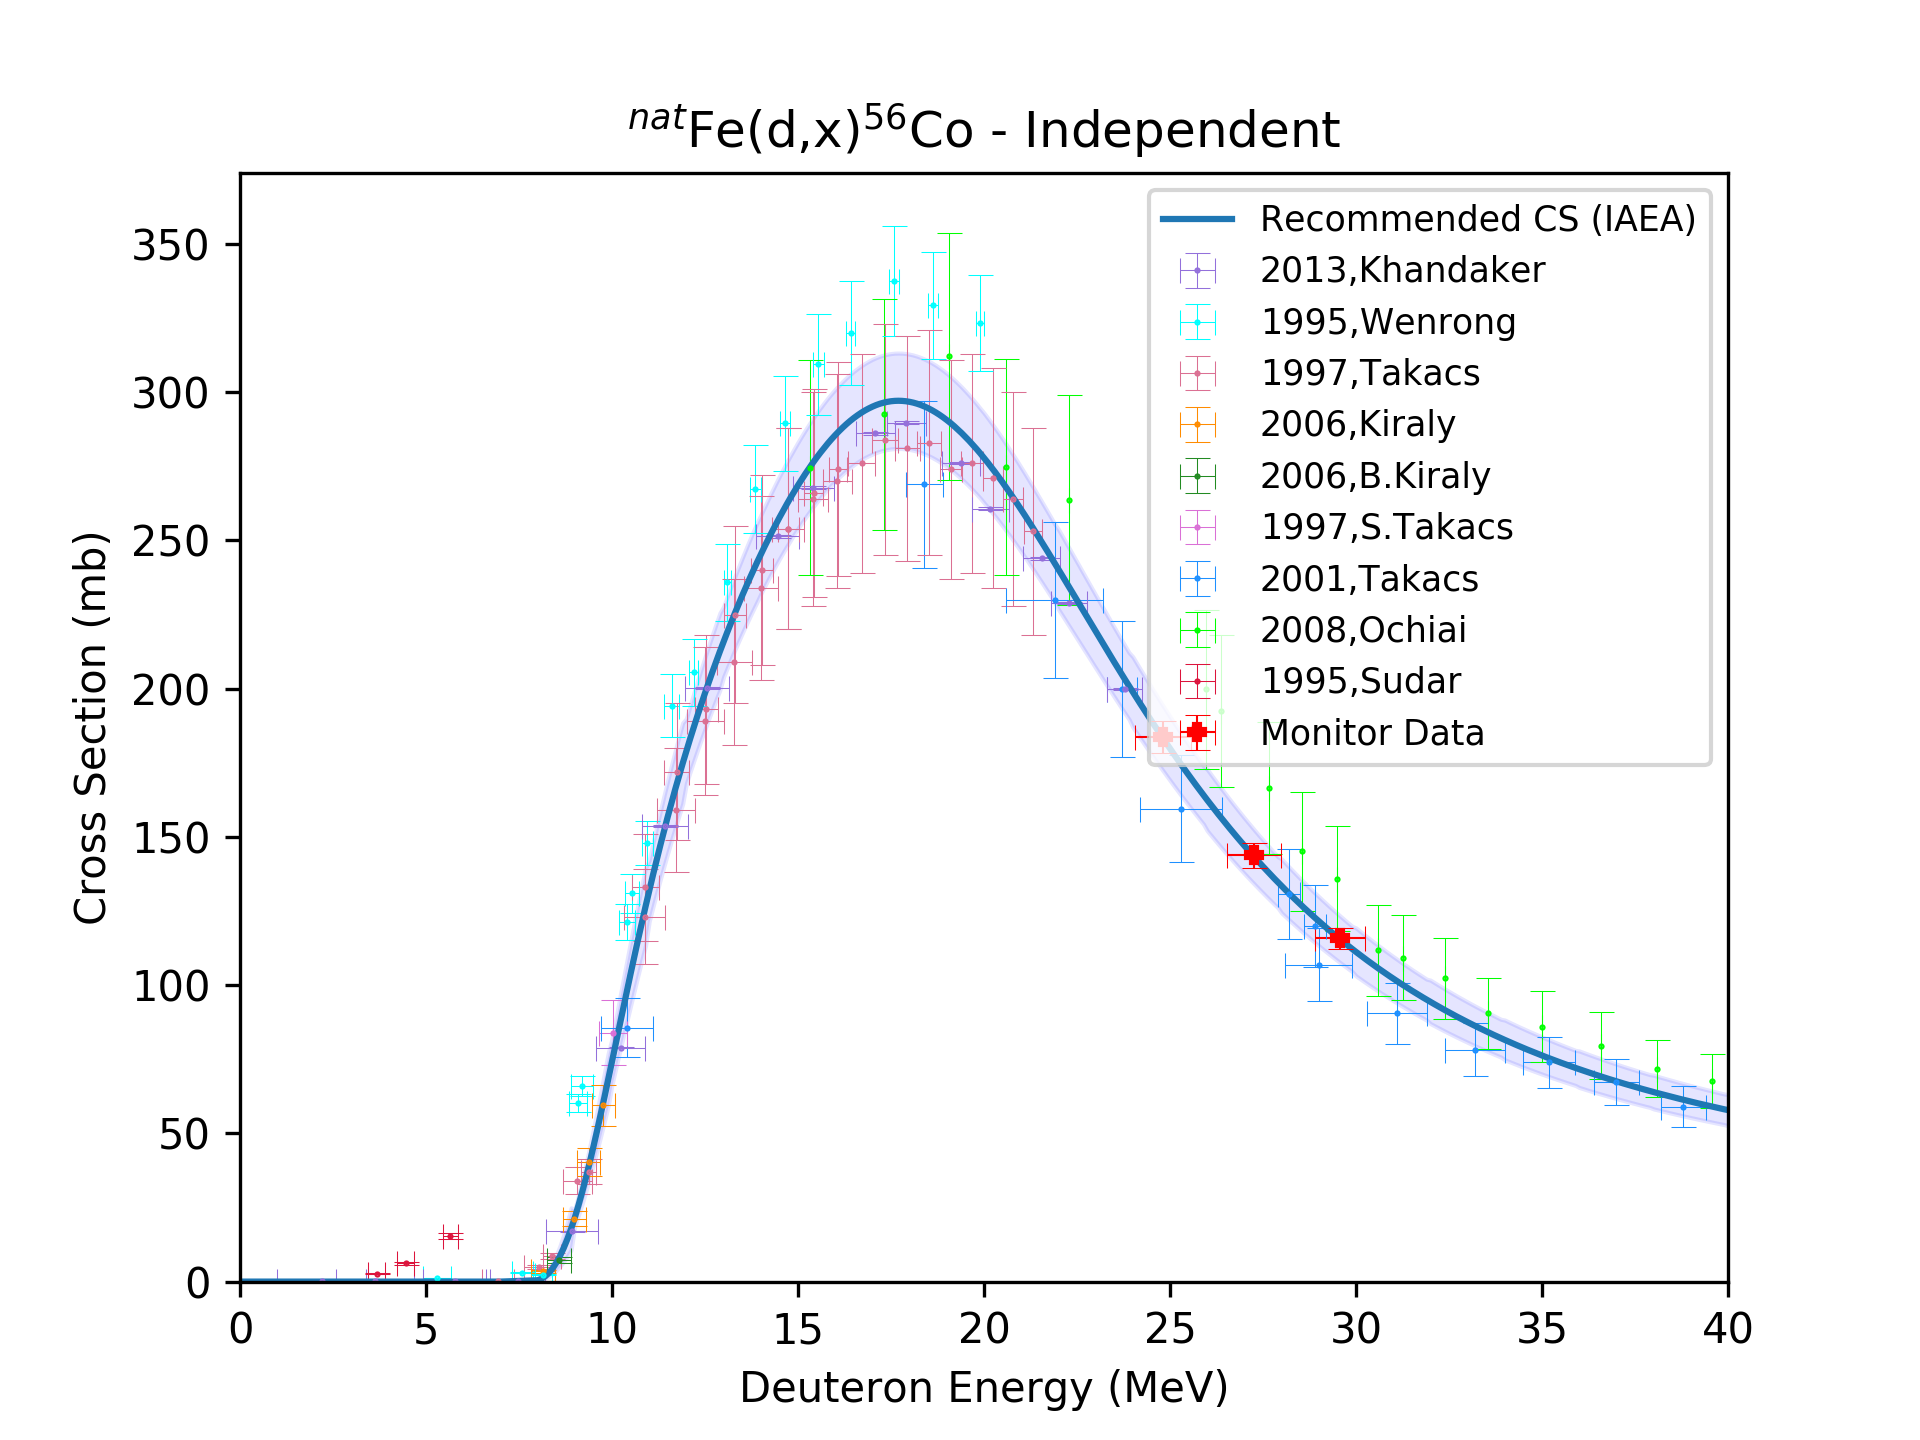
\includegraphics[width=7.5cm]{Analysis/Fe_56Co.png} }}%
    \quad
    \subfloat[]{{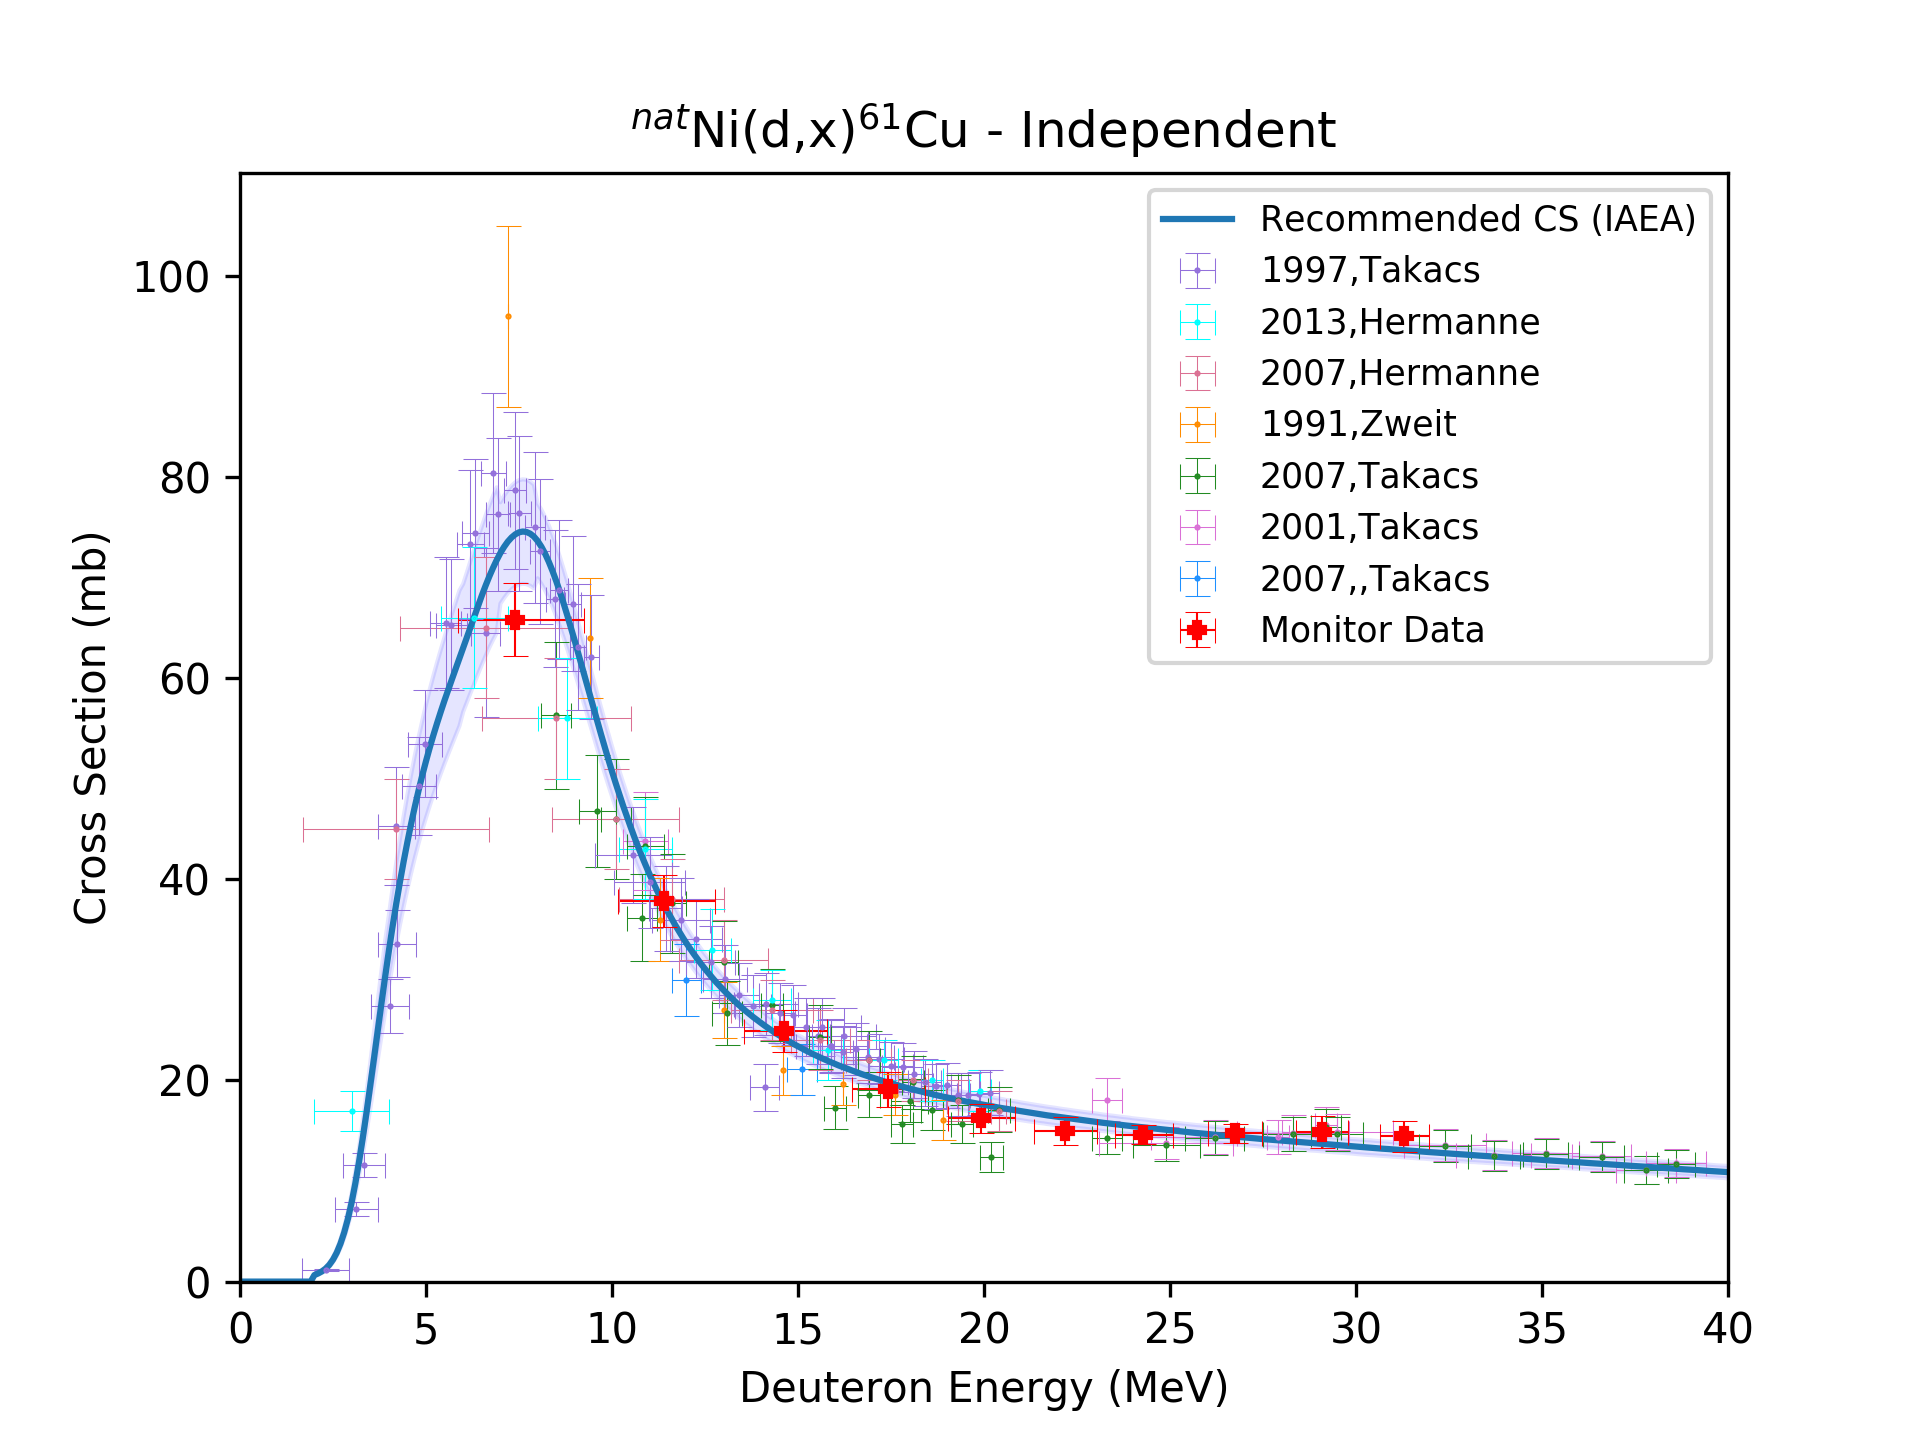
\includegraphics[width=7.5cm]{Analysis/Ni_61Cu.png} }}%
    \subfloat[]{{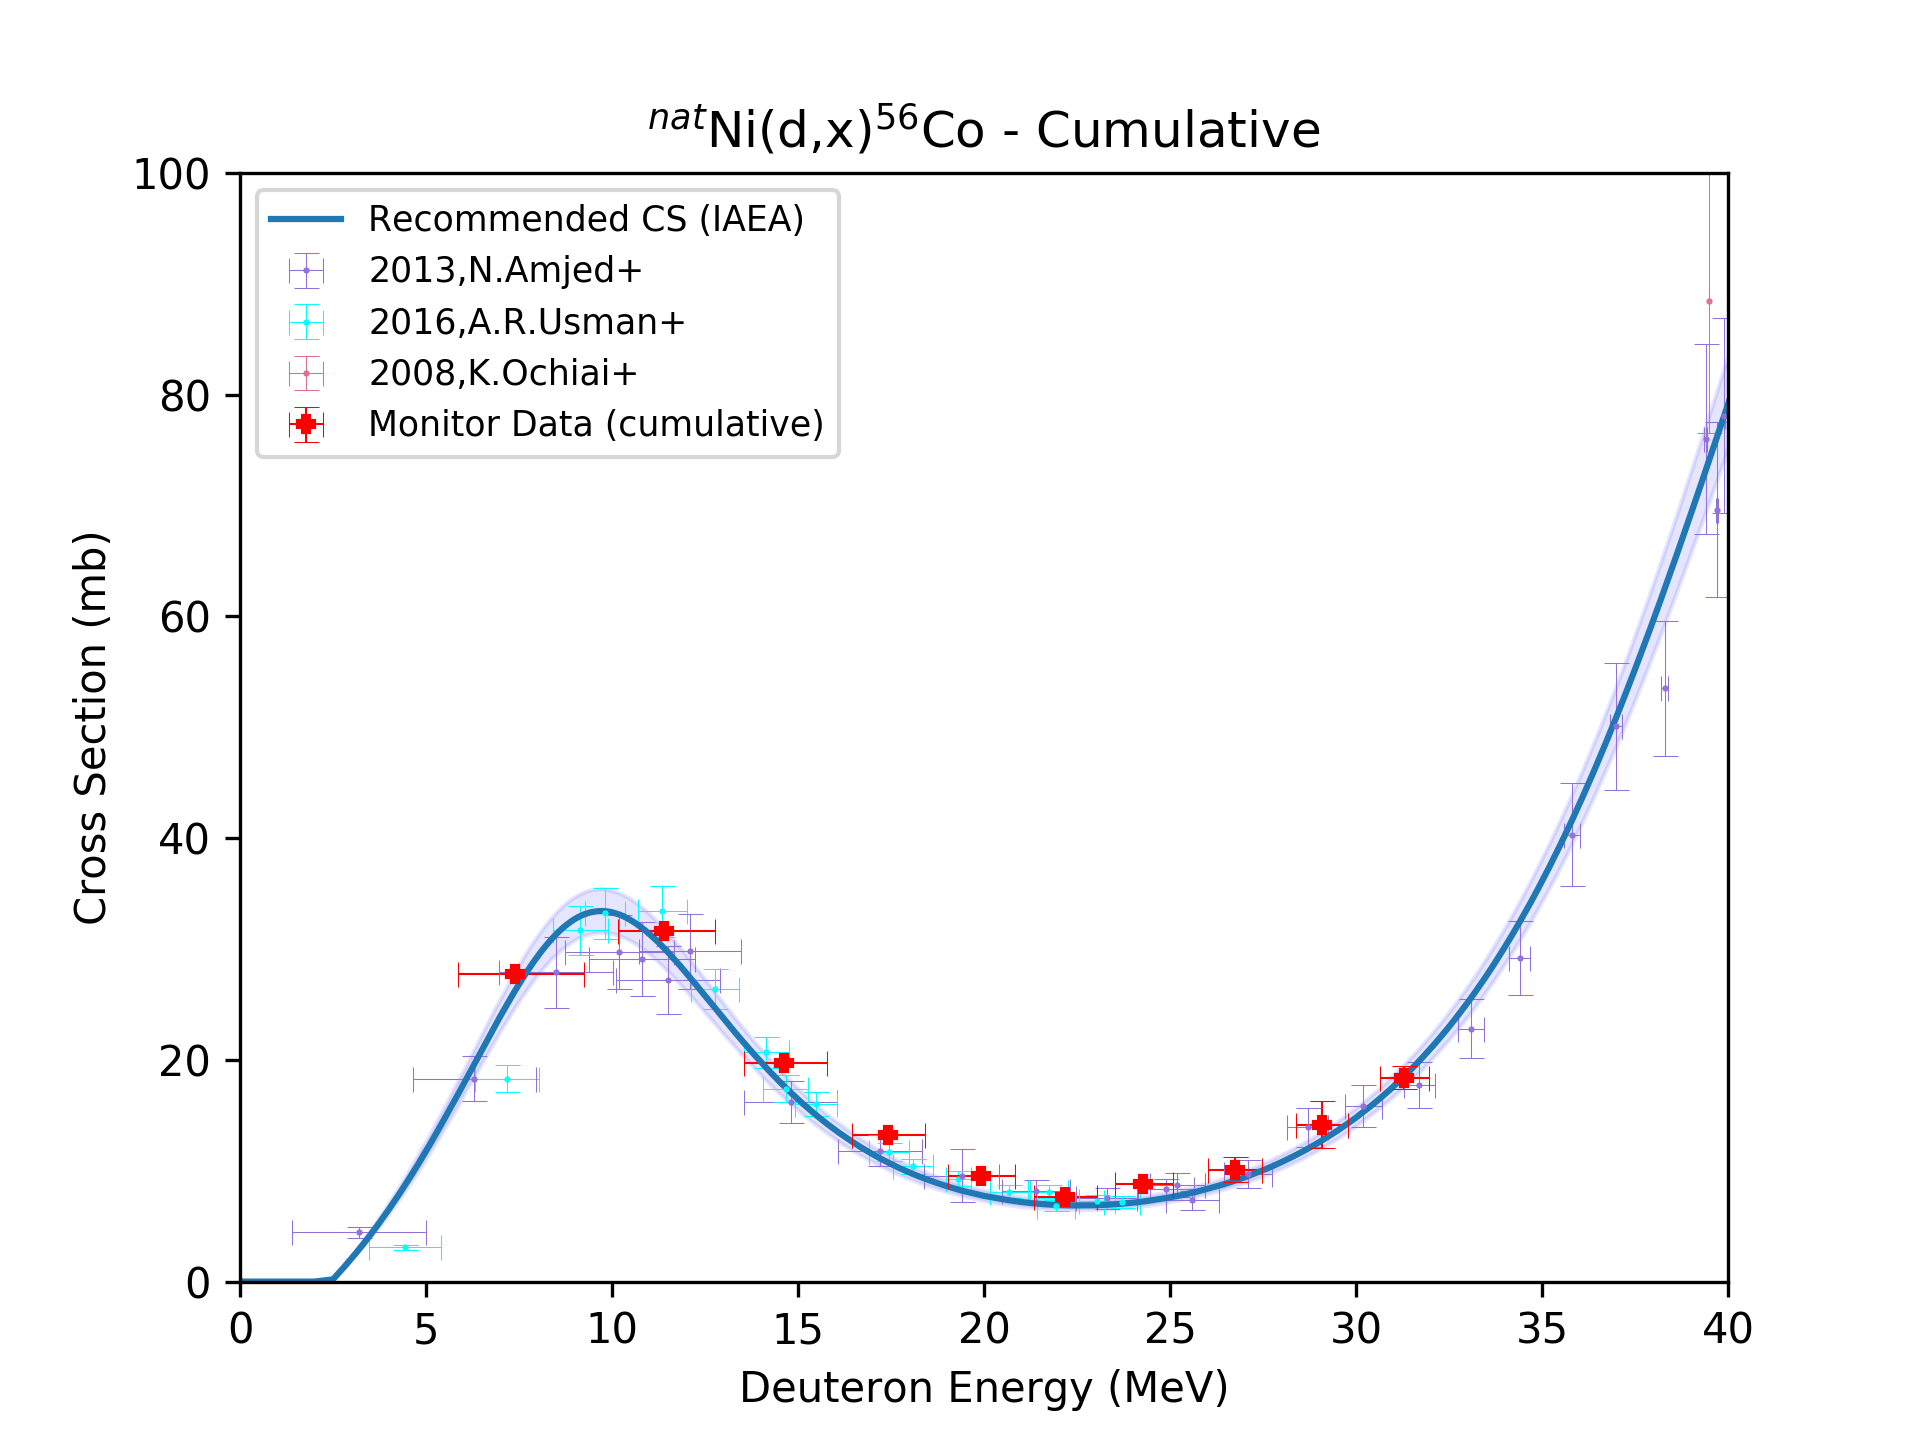
\includegraphics[width=7.5cm]{Analysis/Ni_56Co.png} }}%
    \quad
    \subfloat[]{{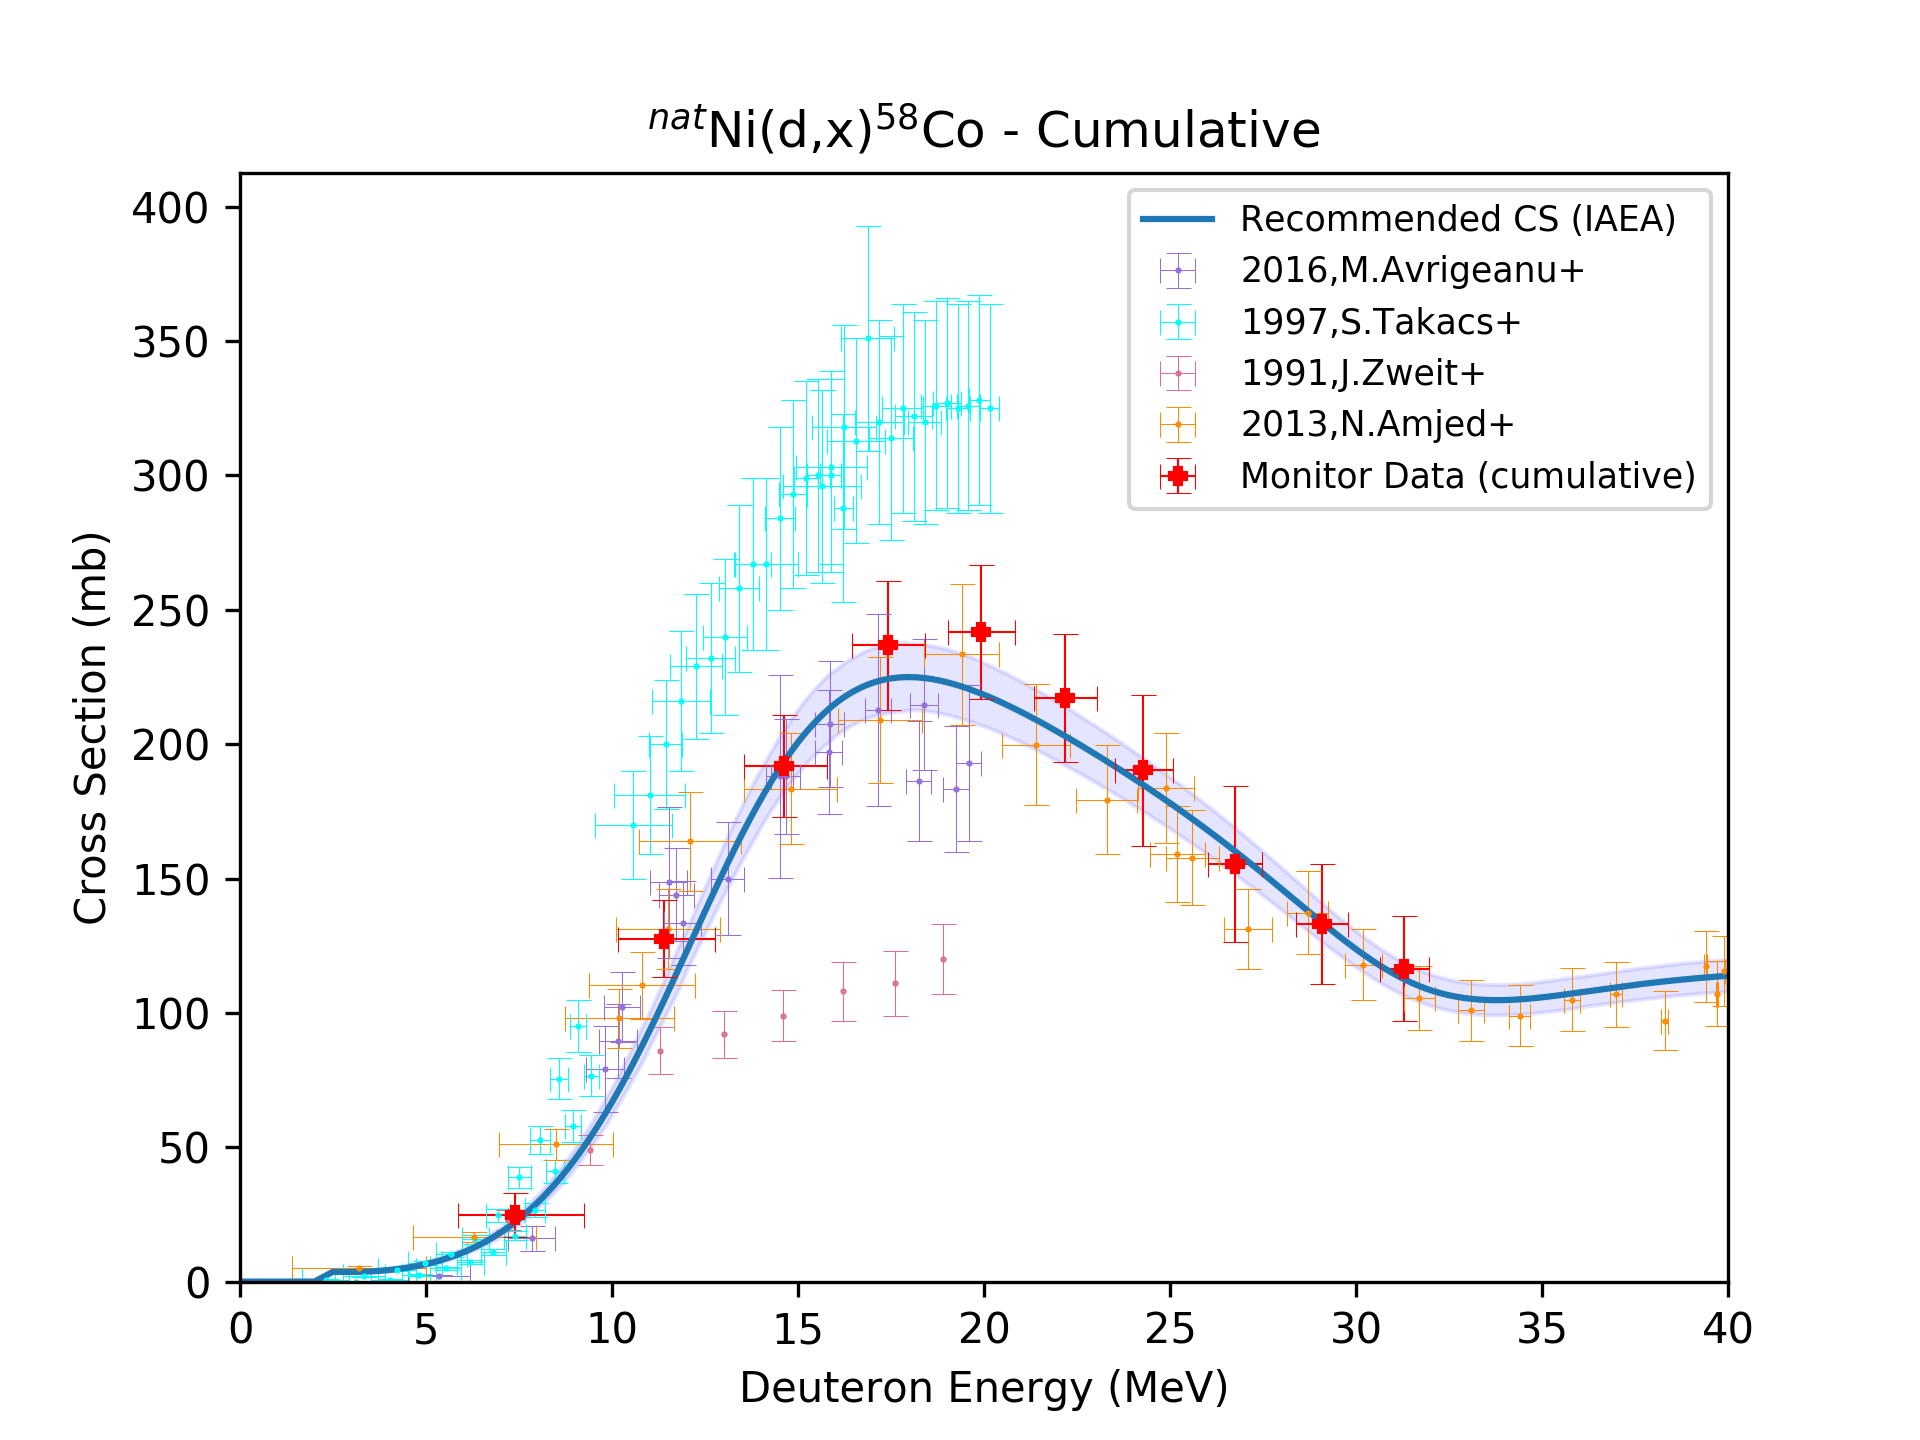
\includegraphics[width=7.5cm]{Analysis/Ni_58Co.png} }}%
    \quad
    \subfloat[caption]{{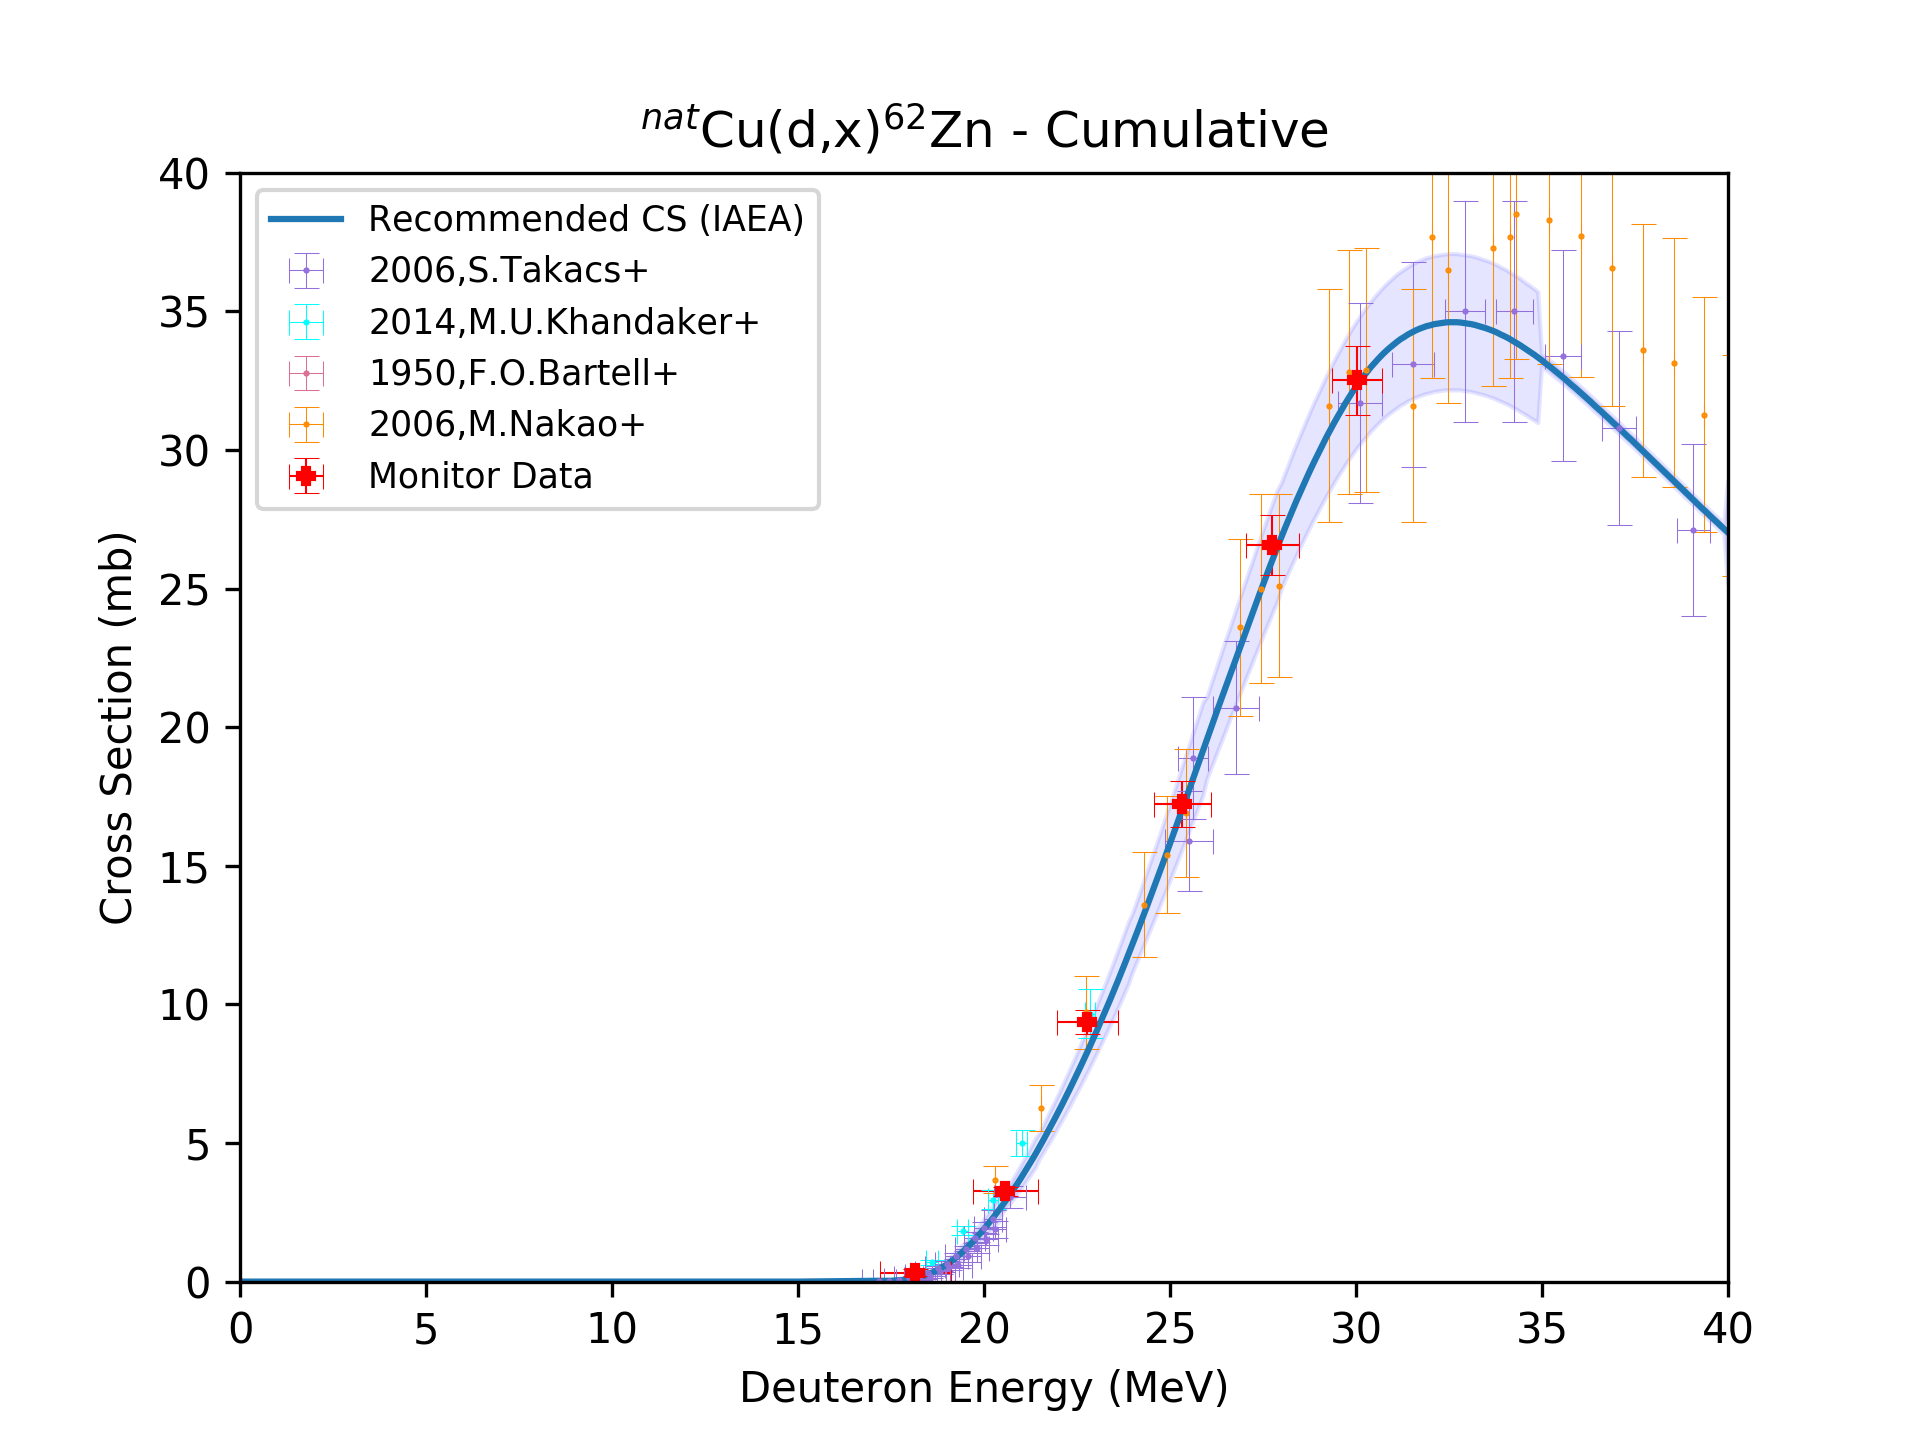
\includegraphics[width=7.5cm]{Analysis/Cu_62Zn.png} }}%
    \quad
    \subfloat[]{{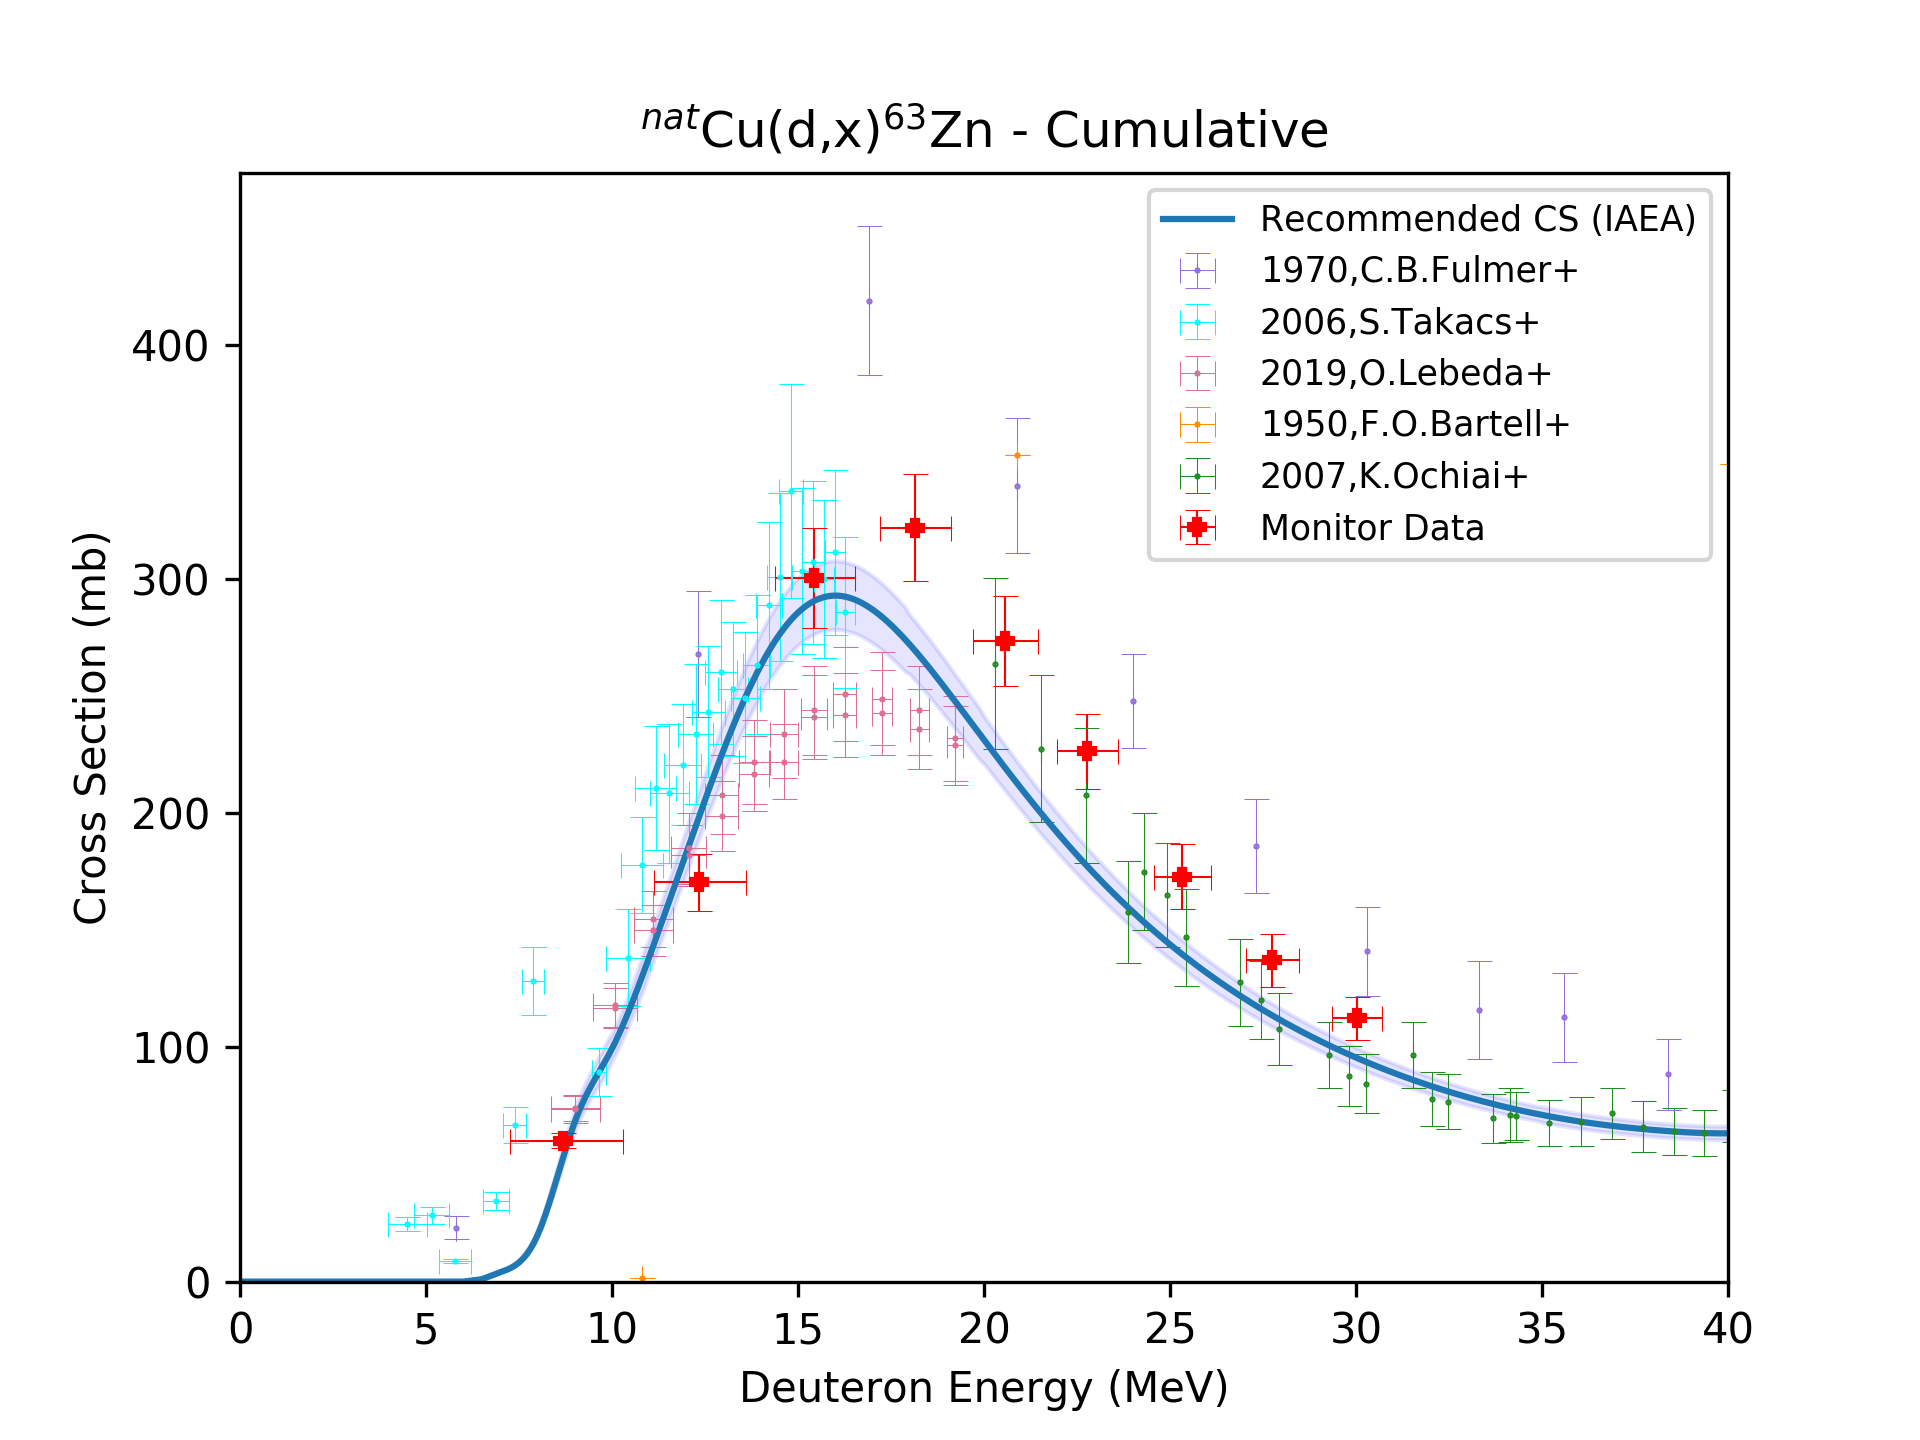
\includegraphics[width=7.5cm]{Analysis/Cu_63Zn.png} }}%
    \quad
    \subfloat[]{{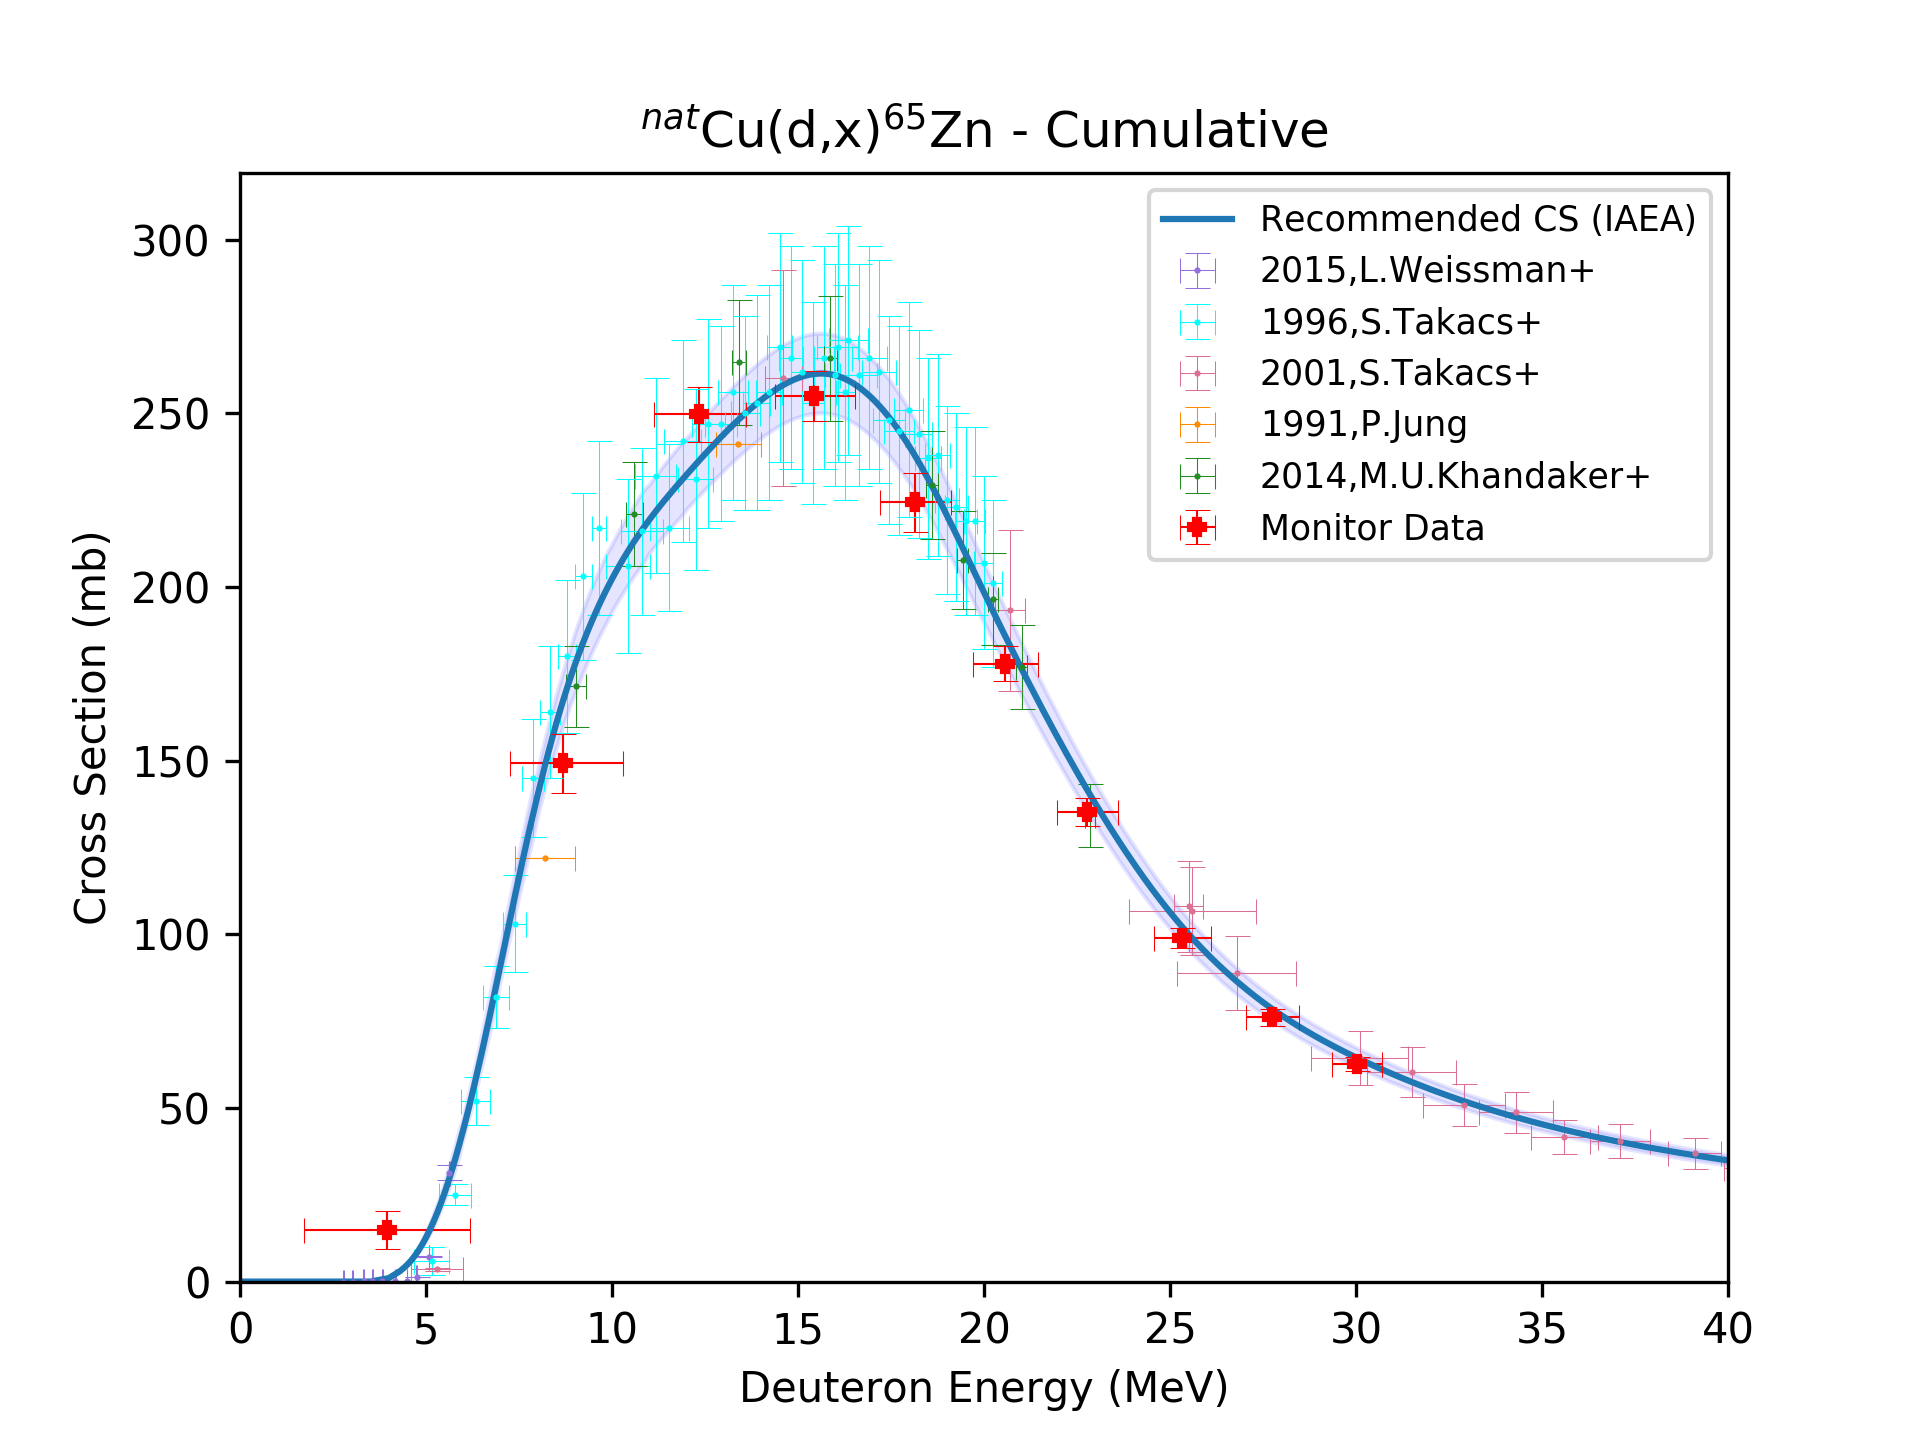
\includegraphics[width=7.5cm]{Analysis/Cu_65Zn.png} }}%
    \quad
    \caption{Figure shows the estimation of monitor cross section using the estimated weighted average beam current for each reaction (not the total). It is compared along with the recommended (IAEA) monitor data, and other experimental data  }%
    \label{fig:monitor_BC+CS}%
\end{figure}

\section{Cross section measurements} 
With all variables for cross sections, cross sections can be calculated using equation \ref{eq:CrossSection_generall}. Since the energy was a flux-weighted average beam energy, the value that is provided as cross section is a flux-averaged cross section. An accurate measure of the cross section as a function of deuteron energy was possible, as the thin foils provides smaller average beam energy intervals, and it makes it possible to have more measurements if thick foils are replaced with several thinner (one single foil represents a single measurement). \textcolor{red}{in theory: Thin foils also produce minimal amounts of radioactivity, thus the deadtime of the detector and the dose to humans is low.}% For charged particles, the stopping power is inversely proportional to their energy\footnote{Andrew S. Voyles, Lee A. Bernstein, Eva R. Birnbaum, Jonathan W. Engle, Stephen A.
%Graves, Toshihiko Kawano, Amanda M. Lewis, and Francois M. Nortier. Excitation functions
%for (p,x) reactions of niobium in the energy range of Ep = 40–90 MeV. Nuclear Instruments
%and Methods in Physics Research Section B: Beam Interactions with Materials and Atoms,
%429:53–74, aug 2018.}, and therefor the energy degradation in thicker foils will be large. For thin targets, we can however assume that the stopping power $dE/dx\simeq 0$, and the cross section can be replaced with a differential (normalized) cross section 
%
%\begin{equation}
%    \sigma(E) = \frac{\int \sigma(E) \frac{d\phi}{dE}dE}{\int \frac{d\phi}{dE}dE}
%\end{equation}

%The energy-limits in the integral can be minimized and the error in the energy for charged particles will be small. \\

\textcolor{blue}{Thin foils decreases the energy width, making a more precise measurement dependent on energy. However the reported cross sections are flux-averaged over the energy distribution subtended by each foil. } 

The cross sections are reported as independent if there is nothing decaying into it (beta feeding or from isomer transition), which means that the first observed element in a decay chain is reported as cumulative unless it is the first possible element (which are the nuclei with one more proton more than the target nuclei, which for this experiment is Platinum (from Ir), Zink (from Cu), Copper (from Ni) and Cobalt (from Fe). If there is feeding, and the half life is much shorter or much longer than the specific nuclei, can choose appropirate timewindow and report as independent, when we know that the feeding has either died out or is very low! 

If possible with feeding: added together to get cumulative or subtracted giving independent. Multiplying by branching ratio. 

The measured cross sections in this work was compared to previous experimental data, along with reaction modelling codes TALYS\foonote{https://sci-hub.tw/https://doi.org/10.1016/j.nds.2012.11.002}, TENDL, ALICE20 and CoH. \\

\noindent 
\textcolor{blue}{from talys cite, p. 2844: Software for the analysis and prediction of nuclear reactions that involve neutrons, photons, protons, deuterons, tritons, $^3$He and alphaparticles, in the 1keV-200 MeV energy range and for target radionuclides of mass 5 and heavier. A suite of nuclear reaction models has been implemented in one single code system. This enables to evaluate nuclear reactions from the unresolved resonance range up to intermediate energies. Can have many different outputs we are interested in exclusive channnel cross sections, energy and double differential spectra p. 2845. 

Optical model calculations performed first, }

Talys takes in projectile, target element (specific isotope or all stable target isotopes), energy array with desired spacing and upper limit energy. 

\textcolor{blue}{from Andrew mail: Each code was ran on default parameters (no changes to nuclear structure or the modeling of the reaction physics). Adjusting allows to tune the code to match experimental data, but this is of limited value as the parameters you settle on to match one product nucleus causes most of the others to get even worse - i.e., its a local optimization, not improving the code globally.  We run our codes for papers on defaults, as 1) that's how 99\% of users do so, and 2) it reveals how good each code's predictive power is. 

For COH: To get both 191Ir and 193Ir to run, we had to adjust the parameter "tweakSD", which adjusts the effective single-particle state density for a particular particle emission channel.  In the end, we ran with tweakSD=0.25  for both outgoing alphas and neutrons  (protons were unaffected).  In other words, we set the single-particle state density for outgoing alphas and neutrons [(d,xa) and (d,xn) reactions]  to be 25\% of what they normally are, which is a HUGE change.} 


\textcolor{blue}{from talys cite p. 2843-2844: TENDL is developed from talys (TALYS evaluated Nuclear data Library).  This
library consists of a complete set of nuclear reaction data
for incident neutrons, photons, protons, deuterons, tritons, Helium-3 and alpha particles, from 10$^−5$ eV up to 200 MeV, for all 2430 isotopes from 6Li to 281Ds that are either stable of have a half-life longer than 1 second.
All data are completely and consistently evaluated using a software system consisting of the TALYS nuclear reaction code, and other software to handle resonance data, experimental data, data from existing evaluations,
and to provide the final ENDF-6 formatting, including
covariance information. The result is a nuclear data library with mutually consistent reaction information for
all isotopes and a quality that increases with yearly updates.  To produce this library, TALYS input parameters are
adjusted for many nuclides so that calculated cross sections agree with experimental data, while for important
nuclides experimental or evaluated data are directly included. Also feedback from integral measurements is
processed into the data libraries. For nuclides for which
(almost) no experimental data exists, default TALYS
calculations based on global models and parameters are
used.}


Dont understand this part..... 

\end{comment}